% Created 2020-06-07 Sun 08:28
% Intended LaTeX compiler: pdflatex

\documentclass[a4paper,12pt]{article}
\usepackage[margin=2cm]{geometry}

\usepackage{hyperref}
\usepackage[utf8]{inputenc}
\usepackage{fixltx2e}
\usepackage{graphicx}
\usepackage{longtable}
\usepackage{float}
\usepackage{wrapfig}
\usepackage{rotating}
\usepackage[normalem]{ulem}
\usepackage{amsmath}
\usepackage{textcomp}
\usepackage{marvosym}
\usepackage{wasysym}
\usepackage{multicol}
\usepackage{amssymb}
\tolerance=1000
\usepackage{listings}
\usepackage[english]{babel}
\addto\captionsenglish{\renewcommand\contentsname{Outline}}
\usepackage[UTF8, heading]{ctex}
\usepackage{xltxtra}
\usepackage{xeCJK}
\usepackage{lmodern}
\usepackage{verbatim}
\usepackage{float}
\usepackage{tikz}
\usepackage{wrapfig}
\usepackage{soul}
\usepackage{textcomp}
\usepackage{listing}
\usepackage{geometry}
\usepackage{algorithm}
\usepackage{algorithmic}
\usepackage{marvosym}
\usepackage{wasysym}
\usepackage{natbib}
\usepackage{fancyhdr}
\usepackage{fontspec,xunicode,xltxtra}
\usepackage{CJKnumb}
\usepackage{amsfonts}
\usepackage[default]{sourcecodepro}
\usepackage[T1]{fontenc}
\setCJKmainfont{SimSun} % 設置缺省中文字體
\setmainfont{Times New Roman} % 英文襯線字體
\setsansfont{Source Code Pro} % 英文無襯線字體
\setmonofont{Source Code Pro} % 英文等寬字體
\setCJKmainfont[Scale=0.9]{Adobe Heiti Std} % 中文字體
\setCJKmonofont[Scale=0.9]{Adobe Heiti Std}
\usepackage{color}
\RequirePackage{fancyvrb}
\usepackage{placeins}
\vspace{-0.2cm}
\usepackage{xcolor}
\hypersetup{pdfauthor={Name},colorlinks,linkcolor={red!50!black},citecolor={blue!50!black},urlcolor={blue!80!black}}
\definecolor{dkgreen}{rgb}{0,0.6,0}
\definecolor{dred}{rgb}{0.545,0,0}
\definecolor{dblue}{rgb}{0,0,0.545}
\definecolor{lgrey}{rgb}{0.9,0.9,0.9}
\definecolor{gray}{rgb}{0.4,0.4,0.4}
\definecolor{darkblue}{rgb}{0.0,0.0,0.6}
\definecolor{bubbles}{rgb}{0.91, 1.0, 1.0}
\definecolor{foreground}{RGB}{220,220,204} % 淺灰
\definecolor{background}{RGB}{62,62,62} % 淺黑
\definecolor{preprocess}{RGB}{250,187,249} % 淺紫
\definecolor{var}{RGB}{239,224,174} % 淺肉色
\definecolor{string}{RGB}{154,150,230} % 淺紫色
\definecolor{type}{RGB}{225,225,116} % 淺黃
\definecolor{function}{RGB}{140,206,211} % 淺天藍
\definecolor{keyword}{RGB}{239,224,174} % 淺肉色
\definecolor{comment}{RGB}{180,98,4} % 深褐色
\definecolor{doc}{RGB}{175,215,175} % 淺鉛綠
\definecolor{comdil}{RGB}{111,128,111} % 深灰
\definecolor{constant}{RGB}{220,162,170} % 粉紅
\lstdefinelanguage{python}{
backgroundcolor=\color{bubbles},
basicstyle=\footnotesize \ttfamily \color{dblue} \small \mono \bfseries,
breakatwhitespace=false,
breaklines=true,
captionpos=b,
comment=[l]{\#},
morecomment=[s]{/*}{*/},
commentstyle=\color{comment} \slshape \small \itshape,
ndkeywords={boolean, throw, import, typeof, null, catch, switch, for, in, int, str, float, self, return, class, if ,elif, endif, while, do, else, True, False , catch, def},
ndkeywordstyle=\color{dred} \bfseries \small \mono,
identifierstyle=\color{black},
deletekeywords={...},
escapeinside={\%*}{*)},
frame=single,
frameround=tttt,
framesep=0pt,
rulecolor=\color{background},
morekeywords={BRIEFDescriptorConfig,string,TiXmlNode,DetectorDescriptorConfigContainer,istringstream,cerr,exit},
identifierstyle=\color{black},
stringstyle=\color{blue},
rulecolor=\color{black},
showspaces=false,
showstringspaces=false,
showtabs=false,
stepnumber=1,
tabsize=5,
title=\lstname,
}
\lstdefinelanguage{shell}{
backgroundcolor=\color{keyword},
basicstyle=\footnotesize \ttfamily \color{dblue} \small \mono \bfseries,
breakatwhitespace=false,
breaklines=true,
captionpos=b,
comment=[l]{\#},
morecomment=[s]{/*}{*/},
commentstyle=\color{comment} \slshape \small \itshape,
identifierstyle=\color{black},
deletekeywords={...},
escapeinside={\%*}{*)},
frame=single,
frameround=tttt,
framesep=0pt,
rulecolor=\color{background},
morekeywords={BRIEFDescriptorConfig,string,TiXmlNode,DetectorDescriptorConfigContainer,istringstream,cerr,exit},
identifierstyle=\color{black},
stringstyle=\color{blue},
rulecolor=\color{black},
showspaces=false,
showstringspaces=false,
showtabs=false,
stepnumber=1,
tabsize=5,
title=\lstname,
}
\usepackage{enumitem}
\setenumerate{noitemsep}
\setenumerate{nolistsep}
\setitemize{nolistsep}
\vspace{-\topsep}
\author{Yung Chin, Yen}
\date{\today}
\title{Advanced Materials of Python}
\begin{document}

\maketitle
\tableofcontents

\newpage
\section{Python 套件管理}
\label{sec:org454d0d3}
\subsection{pip v.s. conda}
\label{sec:org717bf1a}
\begin{enumerate}
\item pip or conda
\label{sec:orgde55b26}
\begin{itemize}
\item Python 的一大優勢之一便是龐大的第三方函式庫，讓使用 python 的程式設計師可以方便的呼叫、進行如網路資料下載解析、資料的視覺化、甚或是大數據的複雜分析與人工智慧的相關套件。，\\
\item 目前用來管理這些龐大套件的工具主要有二：pip 與 Conda。\\
\end{itemize}
\item pip
\label{sec:org35ab7a8}
\begin{itemize}
\item Pip是\href{https://www.pypa.io/en/latest/}{Python Packaging Authority}推薦、用於從\href{https://pypi.org/}{Python Package Index}安裝套件的工具，提供了對 Python 套件的搜㝷、下載、安裝、卸載的功能。\\
\item 若在 python.org 下載最新版本的 python，則已內建 pip 安裝套件。 Python 3.4+ 以上版本均已包括 pip\\
\item 該工具類似 Linux 下的 apt/yum 或 MAC 下的\href{https://brew.sh/index\_zh-tw}{Homebrew}。\\
\end{itemize}
\item conda
\label{sec:org368730d}
\begin{itemize}
\item Conda 是一個開源的跨平台工具軟體，它被設計作為 Python、R、Lua、Scala、C/C++、FORTRAN/ 與 Java 等任何程式語言的套件、依賴性以及工作環境管理員，特別受到以 Python 作為主要程式語言的資料科學團隊所喜愛。\\
\item 適用平台：Windows, macOS, Linux\\
\item 傳統 Python 使用者以 pip 作為套件管理員（package manager）、以 venv 作為工作環境管理員（environment manager），而 conda 則達成了「兩個願望、一次滿足」既可以管理套件亦能夠管理工作環境。\footnote{\href{https://medium.com/datainpoint/python-essentials-conda-quickstart-1f1e9ecd1025}{輕鬆學習 Python：conda 的核心功能}\\\label{org9a526ba}}\\
\end{itemize}
\item In both cases:
\label{sec:orgdc4f94f}
\begin{itemize}
\item Written in Python\\
\item Open source (Conda is BSD and pip is MIT)\\
\item \href{http://inspiregate.com/internet/trends/74-comparison-of-five-kinds-of-standard-open-source-license-bsd-apache-gpl-lgpl-mit.html}{五種開源授權規範的比較 (BSD, Apache, GPL, LGPL, MIT)}\\
\end{itemize}
\item difference between conda, anaconda, and miniconda
\label{sec:org9e1cd09}
\begin{itemize}
\item conda is both a command line tool, and a python package. \footnote{\href{https://stackoverflow.com/questions/30034840/what-are-the-differences-between-conda-and-anaconda}{What are the differences between Conda nd Anaconda?}\\}\\
\item Anaconda 發行版會預裝很多套件，而 Miniconda 是最小的 conda 安裝環境， 一個乾淨的 conda 環境。\\
\item pip  只是運與安裝 python package，而 conda 用來安裝管理任何語言的包。\\
\item 不一定要安裝 Anaconda 或 Miniconda，也可透過 pip 直接安裝 conda\\
\lstset{breaklines=true,language=shell,label= ,caption= ,captionpos=b,numbers=none}
\begin{lstlisting}
  pip install conda
\end{lstlisting}
\end{itemize}
\end{enumerate}

\subsection{conda 安裝與使用}
\label{sec:org7bdb010}
\begin{enumerate}
\item 下載 v.s. 安裝
\label{sec:orgb46ffae}
\begin{itemize}
\item \href{https://www.anaconda.com/distribution/}{Anaconda}\\
\item \href{https://docs.conda.io/en/latest/miniconda.html}{Miniconda}\\
\end{itemize}
\item 移除
\label{sec:org6b8f81d}
\begin{itemize}
\item Windows: uninstall\\
\item Linux/macOS:\\
\lstinline[breaklines=true,language=shell], rm -rf ~/anaconda ,\\
\end{itemize}
\end{enumerate}
\subsection{python package 安裝(conda)}
\label{sec:org71e65d3}
\begin{itemize}
\item 安裝 package:\\
\lstinline[breaklines=true,language=Python]~ conda install packageName ~\\
\lstset{breaklines=true,language=shell,label= ,caption= ,captionpos=b,numbers=none}
\begin{lstlisting}
  conda install pandas
\end{lstlisting}
\item 移除 package:\\
\lstinline[breaklines=true,language=Python]~ conda remove packageName ~\\
\lstset{breaklines=true,language=shell,label= ,caption= ,captionpos=b,numbers=none}
\begin{lstlisting}
  conda remove pandas
\end{lstlisting}
\item 安裝特定版本 python\\
\lstinline[breaklines=true,language=Python]~ conda install python=version ~\\
\lstset{breaklines=true,language=shell,label= ,caption= ,captionpos=b,numbers=none}
\begin{lstlisting}
  conda install python=3.5
\end{lstlisting}
\item 了解目前系統可用套件\\
\lstset{breaklines=true,language=shell,label= ,caption= ,captionpos=b,numbers=none}
\begin{lstlisting}
    conda list
\end{lstlisting}
\end{itemize}
\subsection{Python 常用函式庫}
\label{sec:org205102f}
\begin{enumerate}
\item 爬蟲
\label{sec:orgbe2b76a}
\begin{enumerate}
\item Scrapy:
\label{sec:org7a1064c}
\begin{center}

\includegraphics[width=400]{images/scrapy.jpg}
\end{center}
\begin{itemize}
\item Scrapy，Python 開發的一個快速、高層次的 web 數據抓取框架，用於抓取 web 站點並從頁面中提取結構化的數據。Scrapy 用途廣泛，可以用於數據挖掘、監測和自動化測試\footnote{\href{https://www.google.com/url?sa=t\&rct=j\&q=\&esrc=s\&source=web\&cd=1\&cad=rja\&uact=8\&ved=2ahUKEwjoq476trjpAhUKK6YKHZKAAc8QFjAAegQIAxAB\&url=https\%3A\%2F\%2Fkknews.cc\%2Fzh-tw\%2Fcode\%2F9j99vnl.html\&usg=AOvVaw0eaDh9T-x0LmUEjD4Vq0AX}{分分鐘學會用python爬蟲框架Scrapy爬取心目中女神}\\}。\\
\item Scrapy 吸引人的地方在於它是一個框架，任何人都可以根據需求方便的修改。它也提供了多種類型爬蟲的基類，如 BaseSpider、sitemap 爬蟲等。\\
\end{itemize}
\item beautifulsoup4:
\label{sec:org46d1e20}
\begin{center}

\includegraphics[width=400]{images/bs.png}
\end{center}
\begin{itemize}
\item Beautiful Soup 是一個 Python 的函式庫模組，可以讓開發者僅須撰寫非常少量的程式\\
碼，就可以快速解析網頁 HTML 碼，從中翠取出使用者有興趣的資料、去蕪存菁，降低網\\
路爬蟲程式的開發門檻、加快程式撰寫速度。\footnote{\href{https://blog.gtwang.org/programming/python-beautiful-soup-module-scrape-web-pages-tutorial/}{Python 使用 Beautiful Soup 抓取與解析網頁資料，開發網路爬蟲教學}\\}\\
\item 而 Beautiful Soup 是基於 HTML DOM 的，會載入整個文檔，解析整個 DOM 樹，因此時間和內存開銷都會大很多，所以性能要低於 lxml。\footnote{\href{https://kknews.cc/zh-tw/code/ba95qx6.html}{python爬蟲CSS 選擇器-BeautifulSoup4}\\}\\
\end{itemize}
\item Selenium
\label{sec:org9681610}
\begin{center}

\includegraphics[width=400]{images/selenium.jpg}
\end{center}
\begin{itemize}
\item 原為網頁測試工具，但由於可以直接以程式碼操控瀏覽器的特性，使其成為網路爬蟲必備\\
的工具之一。\footnote{\href{https://freelancerlife.info/zh/blog/python\%E7\%B6\%B2\%E8\%B7\%AF\%E7\%88\%AC\%E8\%9F\%B2\%E6\%95\%99\%E5\%AD\%B8-selenium\%E5\%9F\%BA\%E6\%9C\%AC\%E6\%93\%8D\%E4\%BD\%9C/}{python網路爬蟲教學-Selenium基本操作}\\}\\
\item Selenium 執行「真實的瀏覽器」來進行網站操作的自動化，它能夠直接獲取即時的內容，包括被 JavaScript 修改過的 DOM 內容，讓程式可以直接與網頁元素即時互動、執行 JavaScript 程式，因此也適用於前端採用 AJAX 技術的網站。\footnote{\href{https://learngeb-ebook.readbook.tw/intro/selenium.html}{[認識 Selenium}\\}\\
\item Selenium 是許多 Web Testing 工具的核心，利用 Selenium 操作網頁表單資料、點選按鈕或連結、取得網頁內容並進行檢驗，可以滿足相當多測試的需求。\\
\end{itemize}
\end{enumerate}
\item 網站
\label{sec:org3857136}
\begin{enumerate}
\item Django
\label{sec:org8511c5f}
\begin{center}

\includegraphics[width=400]{images/django.jpg}
\end{center}
\begin{itemize}
\item Django (\emph{ˈdʒæŋɡoʊ} jang-goh) 可以說是 Python 最著名的 Web Framework，一些知名的網站如 Pinterest, Instagram, Disqus 等等都使用過它來開發。\footnote{\href{https://djangogirlstaipei.gitbooks.io/django-girls-taipei-tutorial/django/introduction.html}{Django 介紹}\\}\\
\item 免費開放原始碼\\
\item 著重快速開發、高效能\\
\item 遵從 DRY ( Don't Repeat Yourself ) 守則，致力於淺顯易懂和優雅的程式碼\\
\item 使用類似 Model–view–controller (MVC) pattern 的架構\\
\item \href{https://djangostars.com/blog/10-popular-sites-made-on-django/}{10 Popular Websites Built With Django}\\
\end{itemize}
\item Flask
\label{sec:orga773670}
\begin{center}

\includegraphics[width=400]{images/flask.png}
\end{center}
\begin{itemize}
\item Flask 是一個使用 Python 撰寫的輕量級 Web 應用程式框架，由於其輕量特性，也稱為\\
micro-framework（微框架）。\footnote{\href{https://blog.techbridge.cc/2017/06/03/python-web-flask101-tutorial-introduction-and-environment-setup/}{Python Web Flask 實戰開發教學}\\}\\
\item Flask 和 Django 不同的地方在於 Flask 給予開發者非常大的彈性（當然你也可以說是\\
需要思考更多事情），可以選用不同的用的 extension 來增加其功能。\\
\item 相比之下，Django 雖然完善但技術選擇相對不彈性，不論是 ORM、表單驗證或是模版引\\
擎都有自己的作法。\\
\item 沒有最好的框架，只有合適的使用情境。\\
\end{itemize}
\end{enumerate}
\item 資料處理科學計算
\label{sec:org428fd31}
\begin{enumerate}
\item Numpy
\label{sec:orga7c68e8}
\begin{center}

\includegraphics[width=400]{images/numpy.jpg}
\end{center}
\begin{itemize}
\item Numpy 底層以 C 和 Fortran 語言實作，所以能快速操作多重維度的陣列。\footnote{\href{https://blog.techbridge.cc/2017/07/28/data-science-101-numpy-tutorial/}{從零開始學資料科學：Numpy 基礎入門}\\}\\
\item 當 Python 處理龐大資料時，其原生 list 效能表現並不理想（但可以動態存異質資料），而 Numpy 具備平行處理的能力，可以將操作動作一次套用在大型陣列上。\\
\item 此外 Python 其餘重量級的資料科學相關套件（例如：Pandas、SciPy、Scikit-learn 等）都幾乎是奠基在 Numpy 的基礎上。\\
\end{itemize}
\item Scipy
\label{sec:org6150e43}
\begin{center}

\includegraphics[width=400]{images/scipy.png}
\end{center}
\begin{itemize}
\item 科學計算神器\\
\item Numpy 是以矩陣基礎做數據的數學運算，SciPy 就是以 Numpy 為基礎做科學、工程的運算處理的 package，包含統計、優化、整合、線性代數、傅立葉轉換圖像等較高階的科學運算。\footnote{\href{https://ithelp.ithome.com.tw/articles/10193295}{[Day05]聊聊重要的三個package吧！ }\\}\\
\end{itemize}
\item Pandas
\label{sec:orgbbe7b96}
\begin{center}

\includegraphics[width=400]{images/pandas.png}
\end{center}
\begin{itemize}
\item 建構在 NumPy 之上，提供資料結構與資料處理工具，讓資料清理與分析更為快速與方便\\
\item 適合處理表格或異質資料 (NumPy 適合處理同質之數值陣列資料)\\
\end{itemize}
\end{enumerate}
\item 視覺化
\label{sec:org5c3ac08}
\begin{enumerate}
\item matplotlib
\label{sec:orgaff792f}
\begin{center}

\includegraphics[width=400]{images/matplotlib.jpg}
\end{center}
\begin{itemize}
\item Matplotlib 就是 MATLAB+Plot+Library 的簡稱，因為是模仿 MATLAB 建立的繪圖庫，所以繪\\
圖風格會與 MATLAB 有點類似。\footnote{\href{https://medium.com/python-\%E8\%B3\%87\%E6\%96\%99\%E8\%A6\%96\%E8\%A6\%BA\%E5\%8C\%96/python-\%E5\%95\%86\%E6\%A5\%AD\%E6\%95\%B8\%E6\%93\%9A\%E5\%88\%86\%E6\%9E\%90\%E8\%88\%87\%E5\%8F\%AF\%E8\%A6\%96\%E5\%8C\%96\%E7\%B9\%AA\%E5\%9C\%96-3-1\%E8\%AC\%9B-matplotlib-\%E4\%BB\%8B\%E7\%B4\%B9-e1928f7dfd35}{[Python 商業數據分析之可視化繪圖] 第3.1講：Matplotlib 介紹}\\}\\
\item 為了提高處理大量資料的性能，Matplotlib 大量使用了 NumPy 和其相關的擴展代碼。 為了方便快速繪圖， Matplotlib 通過 pyplot 模組提供了一套和 MATLAB 類似的繪圖 API，只需要調用 pyplot 模組所提供的函數，就可以實現快速繪圖及設置圖表的各種細節。\\
\item 另一方面 Matplotlib 也適合互動式繪製圖表，可以很方便地處理二維和三維的圖表。\\
\end{itemize}
\item seaborn
\label{sec:org93c7141}
\begin{center}

\includegraphics[width=400]{images/seaborn.png}
\end{center}
\begin{center}
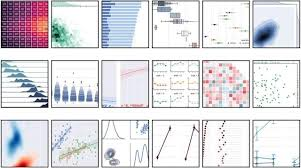
\includegraphics[width=400]{images/seabornPlots.jpg}
\end{center}
\begin{itemize}
\item 散點圖矩陣神器\\
\item Seaborn 是 Python 一個著名的數據視覺化的 package, 以 matplotlib 為基底的一個擴\\
展包, 它提供了易於理解的統計圖和便利的繪圖指令\footnote{\href{https://killer0001.blogspot.com/2018/09/1-seaborn.html}{ Seaborn 介紹 }\\}\\
\item seaborn 庫是對 matplotlib 庫更高級別的封裝，相當於提供了各種統計圖的模板\footnote{\href{https://kknews.cc/zh-tw/code/9z88248.html}{python數據可視化（一）seaborn介紹及繪圖風格設置}\\}\\
\end{itemize}
\item ggplot
\label{sec:orgab25ef8}
\begin{center}

\includegraphics[width=300]{images/ggplot.jpg}
\end{center}
\begin{itemize}
\item R 語言視覺化神器的 Python 版本\\
\item ggplot2 是一個十分強大的 R 語言可視化包。它的核心理念是將繪圖與數據分離，數據相關\\
的繪圖與數據無關的繪圖分離。\footnote{\href{https://www.lizenghai.com/archives/65323.html}{R語言ggplot2系列1-ggplot2簡介}\\}\\
\item 它是按圖層作圖的，一個語句做一個僅包含基礎作圖單元的圖層，然後通過不同圖層的疊\\
加最後成圖。\\
\end{itemize}
\item plotly
\label{sec:orgc37620d}
\begin{center}

\includegraphics[width=400]{images/plotly.png}
\end{center}
\begin{itemize}
\item 這個神器是個 js 庫，不過也有各種流行的語言介面\\
\item plotly 是一個能讓你畫出互動式圖表的一個開源套件,其基本操作是免費的,如果你想要使用網頁的版本,可以使用更多 plotly 的進階功能的話,就必須付費\\
\end{itemize}
\end{enumerate}
\item 機器學習
\label{sec:orge6bca9d}
\begin{enumerate}
\item scikit-learn
\label{sec:org38e75fb}
\begin{center}

\includegraphics[width=400]{images/scikit-learn.png}
\end{center}
\begin{itemize}
\item 幾乎所有機器學習演算法都囊括\\
\item scikit-learn，又寫作 sklearn，是一個開源的基於 python 語言的機器學習工具包。它通\\
過 NumPy, SciPy 和 Matplotlib 等 python 數值計算的庫實現高效的算法應用，並且涵蓋了幾\\
乎所有主流機器學習算法。\footnote{\href{https://www.itread01.com/content/1551725786.html}{機器學習入門之sklearn介紹}\\}\\
\item sklearn 中常用的 module 有分類、回歸、聚類、降維、模型選擇、預處理。\\
\end{itemize}
\item NLTK
\label{sec:orge422034}
\begin{center}

\includegraphics[width=300]{images/NLTK.png}
\end{center}
\begin{itemize}
\item NLTK 全文是 “Nature Language Tool Kit” (NLTK)，是 Python 中一個經典的、專門用於進行自然語言處理的工具。\footnote{\href{https://clay-atlas.com/blog/2019/07/30/\%E3\%80\%90nlp\%E3\%80\%91nltk-\%E5\%9F\%BA\%E6\%9C\%AC\%E6\%95\%99\%E5\%AD\%B8/}{英文自然語言處理的經典工具: NLTK}\\}\\
\item 雖然也能進行部份中文的處理，但是對於中文的支援度自然沒有英文來得好\\
\item 目前而言，繁體中文有兩個套件可以使用，一個是中研院開發的斷詞系統，另一套系統為\\
jieba(結巴)。\\
\item \href{https://poem.msxiaobing.com/}{少女詩人小冰}\\
\end{itemize}
\item TensorFlow
\label{sec:orgf1ebf47}
\begin{center}

\includegraphics[width=400]{images/tensorflow.jpg}
\end{center}
\begin{itemize}
\item Tensorflow 最初為 Google Brian 所開發。在 2015 時，Google 將之開源，為現今重要的深\\
度學習框架之一，它支援各式不同的深度學習演算法，並已應用於各大企業服務上，Ex:\\
Google, Youtube, Airbnb, Paypal \ldots{} 等。\footnote{\href{https://ithelp.ithome.com.tw/articles/10215969?sc=iThelpR}{[Day-1] Tensorflow 介紹 及 Tensorflow 2.0相關知識 }\\}\\
\item 此外，Tensorflow 也支援在各式不同的\\
device 上運行深度學習 Ex: Tensorflow Lite 、 Tensorflow.js 等等。\\
\item Tensorflow 為目\\
前最受歡迎的機器學習、深度學習開源專案。不管是 github fork 的數量、論文的使用次\\
數以及熱門程度，均比其他的框架來的多\footnote{\href{https://towardsdatascience.com/deep-learning-framework-power-scores-2018-23607ddf297a}{Deep Learning Framework Power Scores 2018\\
}\\}。\\
\end{itemize}

深度學習套件\\
\item Keras
\label{sec:org206a973}
\begin{center}

\includegraphics[width=400]{images/keras.png}
\end{center}
\begin{itemize}
\item 在 2015 年 TensorFlow 推出的同時，美國麻省理工學院（又是它，這學校開門就能賺錢）\\
也推出一套能很容易被使用者透過 Python 寫 Deep learning 的應用程式介面 API ，叫\\
做 Keras 。\\
\item Keras 只有介面喔！ \href{https://www.math.ntnu.no/emner/TMA4268/2018v/11NN/3-keras.html}{Keras 本身還是得透過 TensorFlow ，或者其\\
他像是微軟的 CNTK 這類引擎當作底層，才能執行}。\footnote{\href{https://makerpro.cc/2019/06/self-learning-series5-of-ai/}{【自學AI\#5】深度學習必備：Keras、Jupyter安裝教學}\\}\\
\item Keras 使用上比較接近人類的想法（ TensorFlow 設計上沒有錯，只不過比較是針對電腦\\
系統跟網路通訊的想法），所以透過 Python 呼叫 Keras 能夠很簡單地描述我們人類想\\
要電腦達到 Deep Learning 要做的事情。目前在教學上， Keras 的普及率相當高\\
\item Keras 可以快速有方便運算的主要原因是，它已經將訓練模型的輸入層、隱藏層、輸出層，做好架構，使用者只需要加入並且填寫正確的參數 ex.神經元個數、activation function 的函式…等。\footnote{\href{https://medium.com/chiukevin0321/tensorflow\%E8\%88\%87keras\%E5\%9F\%BA\%E6\%9C\%AC\%E4\%BB\%8B\%E7\%B4\%B9-621352fc7150}{Tensorflow與Keras基本介紹}\\}\\
\end{itemize}
\item PyTorch
\label{sec:org5f8a3c6}
\begin{center}

\includegraphics[width=400]{images/pytorch.jpg}
\end{center}
\begin{itemize}
\item Numpy 的 GPU 版\\
\item PyTorch 為 Facebook 在 2017 年初開源的深度學習框架，其建立在 Torch 之上，且標\\
榜 Python First ，為量身替 Python 語言所打造，使用起來就跟寫一般 Python 專案沒\\
兩樣，也能和其他 Python 套件無痛整合。PyTorch 的優勢在於其概念相當直觀且語法簡\\
潔優雅，因此視為新手入門的一個好選項；再來其輕量架構讓模型得以快速訓練且有效運\\
用資源。\footnote{\href{https://medium.com/pyladies-taiwan/\%E6\%B7\%B1\%E5\%BA\%A6\%E5\%AD\%B8\%E7\%BF\%92\%E6\%96\%B0\%E6\%89\%8B\%E6\%9D\%91-pytorch\%E5\%85\%A5\%E9\%96\%80-511df3c1c025}{深度學習新手村：PyTorch入門}\\}\\
\item 於 PyTorch 框架中，資料類型定義為張量(Tensor)，張量可以是純量、向量或是更高維度的矩陣，而 torch 函式庫負責張量在 CPU/GPU 的運算。\\
\end{itemize}
\end{enumerate}
\end{enumerate}
\subsection{python 執行環境建立與維護}
\label{sec:org6ce533d}
\begin{itemize}
\item 建立\footnote{\href{https://ithelp.ithome.com.tw/articles/10192460}{Day01 Anaconda環境安裝!}\\\label{org43bd2be}}\\
\lstset{breaklines=true,language=shell,label= ,caption= ,captionpos=b,numbers=none}
\begin{lstlisting}
conda create -n envName
\end{lstlisting}
\item 啟用\\
\lstset{breaklines=true,language=shell,label= ,caption= ,captionpos=b,numbers=none}
\begin{lstlisting}
conda activate envName
\end{lstlisting}
\item 退出\\
\lstset{breaklines=true,language=shell,label= ,caption= ,captionpos=b,numbers=none}
\begin{lstlisting}
 conda deactiveate
\end{lstlisting}
\item 刪除\\
\lstset{breaklines=true,language=shell,label= ,caption= ,captionpos=b,numbers=none}
\begin{lstlisting}
conda env remove -n envName
\end{lstlisting}
\item 列出目前系統中所有的虛擬環境\\
\lstset{breaklines=true,language=shell,label= ,caption= ,captionpos=b,numbers=none}
\begin{lstlisting}
conda env list
\end{lstlisting}
\end{itemize}
\subsection{將執行環境匯入 jupyter}
\label{sec:org27992a3}
\begin{itemize}
\item 於終端機(for windows: Anaconda prompt)下建立、啟用所需虛擬環境\\
\item 將環境滙至 jupyter kernel\\
\end{itemize}
\lstset{breaklines=true,language=shell,label= ,caption= ,captionpos=b,numbers=none}
\begin{lstlisting}
python -m ipykernel install --user --name 虛擬環境名稱 --display-name "在jupyter中的名稱"
\end{lstlisting}
\begin{itemize}
\item 啟動 jupyter\\
\end{itemize}
\newpage

\section{Numpy}
\label{sec:org6006197}
\subsection{關於 Numpy}
\label{sec:org5b764d6}
\begin{itemize}
\item Numpy 是 Python 的一個重要模組，主要用於資料處理上。Numpy 底層以 C 和 Fortran 語言實作，所以能快速操作多重維度的陣列。\footnote{\href{https://blog.techbridge.cc/2017/07/28/data-science-101-numpy-tutorial/}{從零開始學資料科學：Numpy 基礎入門}\\\label{orgc4061f5}}\\
\item 當 Python 處理龐大資料時，其原生 list 效能表現並不理想（但可以動態存異質資料），而 Numpy 具備平行處理的能力，可以將操作動作一次套用在大型陣列上。\\
\item Python 多數重量級的資料科學相關套件（例如：Pandas、SciPy、Scikit-learn 等）都幾乎是奠基在 Numpy 的基礎上。因此學會 Numpy 對於往後學習其他資料科學相關套件打好堅實的基礎。\\
\end{itemize}
\subsection{匯入模組}
\label{sec:orgb19a2c1}
\begin{itemize}
\item 使用模組裡的函式要加模組名稱\\
\lstset{breaklines=true,language=Python,label= ,caption= ,captionpos=b,numbers=none}
\begin{lstlisting}
    import numpy
\end{lstlisting}
\item 匯入 numpy 模組並使用 np 作為簡寫，這是 Numpy 官方倡導的寫法\\
\lstset{breaklines=true,language=Python,label= ,caption= ,captionpos=b,numbers=none}
\begin{lstlisting}
    import numpy as np
\end{lstlisting}
\item Numpy 中的多維資料型別稱為 ndarray\\
\end{itemize}
\subsection{Create ndarray}
\label{sec:org345fa6d}
\begin{itemize}
\item Numpy 的重點在於陣列的操作，其所有功能特色都建築在同質且多重維度的 ndarray（N-dimensional array）上。\\
\item ndarray 的關鍵屬性是維度（ndim）、形狀（shape）和數值類型（dtype）。 一般我們稱一維陣列為 vector 而二維陣列為 matrix\textsuperscript{\ref{orgc4061f5}}。\\
\end{itemize}
\begin{enumerate}
\item 一維陣列
\label{sec:org0f7e1df}
\begin{itemize}
\item list 或 tuple 轉入\\
\lstset{breaklines=true,language=Python,label= ,caption= ,captionpos=b,firstnumber=1,numbers=left}
\begin{lstlisting}
    import numpy as np
    np1 = np.array( [1, 2, 3, 4] )
    print(np1)
\end{lstlisting}

\begin{results}
\end{results}

\item 使用 np.arange( ) 方法\\
\lstset{breaklines=true,language=Python,label= ,caption= ,captionpos=b,firstnumber=1,numbers=left}
\begin{lstlisting}
  import numpy as np
  np2 = np.arange(5)
  print(np2)
\end{lstlisting}

\item np.arange() v.s. range()\\
\url{PythonBasic.org}\\
差異：\\
\begin{itemize}
\item range()為 python 內建函數\\
\item range() return 的是 range object，而 np.nrange() return 的是 numpy.ndarray()\\
\item range()不支援 step 為小數，np.arange()支援 step 為小數\\
\end{itemize}
\end{itemize}

\item 二維陣列
\label{sec:org516a7b9}
\lstset{breaklines=true,language=Python,label= ,caption= ,captionpos=b,firstnumber=1,numbers=left}
\begin{lstlisting}
import numpy as np

np4 = np.array( [[1, 2, 4], [3, 4, 5]] )
print("shape:", np4.shape)
print("np4:\n", np4)
print("取出第0列:",np4[0])
print("取出第1行:",np4[:,1])
np5 = np.array([np.arange(3), np.arange(3)])
print('np5:\n', np5)

np6 = np.arange(8).reshape(2, 4)
print('np6:\n', np6)
\end{lstlisting}

\begin{verbatim}
  shape: (2, 3)
  np4:
   [[1 2 4]
   [3 4 5]]
  取出第0列: [1 2 4]
  取出第1行: [2 4]
  np5:
   [[0 1 2]
   [0 1 2]]
  np6:
   [[0 1 2 3]
   [4 5 6 7]]
\end{verbatim}
\item 多維陣列
\label{sec:orgbf35092}
\lstset{breaklines=true,language=Python,label= ,caption= ,captionpos=b,firstnumber=1,numbers=left}
\begin{lstlisting}
import numpy as np

np7 = np.arange(24).reshape(2, 3, 4)
print('np7:\n',np7)

np8 = np.arange(13, 60, 2).reshape(2, 3, 4)
print("np8:\n", np8)
\end{lstlisting}

\begin{verbatim}
  np7:
   [[[ 0  1  2  3]
    [ 4  5  6  7]
    [ 8  9 10 11]]

   [[12 13 14 15]
    [16 17 18 19]
    [20 21 22 23]]]
  np8:
   [[[13 15 17 19]
    [21 23 25 27]
    [29 31 33 35]]

   [[37 39 41 43]
    [45 47 49 51]
    [53 55 57 59]]]
\end{verbatim}
\item 隨機矩陣
\label{sec:orga9683b2}
\lstset{breaklines=true,language=Python,label= ,caption= ,captionpos=b,firstnumber=1,numbers=left}
\begin{lstlisting}
import numpy as np

np8 = np.random.random((3, 2)) #矩陣大小以tuple表示
print('np8:\n', np8)

np9 = np.random.randint(0, 100, size=[4, 3]) #矩陣大小以list表示
print('np9:\n', np9)
\end{lstlisting}

\begin{verbatim}
np8:
 [[0.6245669  0.32882812]
 [0.77169389 0.53843892]
 [0.02838865 0.60851828]]
np9:
 [[14 45 43]
 [79 64 47]
 [32 76 28]
 [53  8 18]]
\end{verbatim}


\item 0/1 矩陣
\label{sec:orge7f3fbb}
\begin{itemize}
\item np.zeros: np.zeros( (陣列各維度大小用逗號區分) )：建立全為 0 的陣列，可以小括號定義陣列的各個維度的大小\\
\end{itemize}
\lstset{breaklines=true,language=Python,label= ,caption= ,captionpos=b,firstnumber=1,numbers=left}
\begin{lstlisting}
import numpy as np

zeros = np.zeros( (3, 5) )
print("zeros=>\n{0}".format(zeros))
\end{lstlisting}

\begin{verbatim}
zeros=>
[[0. 0. 0. 0. 0.]
 [0. 0. 0. 0. 0.]
 [0. 0. 0. 0. 0.]]
\end{verbatim}


\begin{itemize}
\item np.ones: np.ones( (陣列各維度大小用逗號區分) )：用法與 np.zeros 一樣\\
\end{itemize}
\lstset{breaklines=true,language=Python,label= ,caption= ,captionpos=b,firstnumber=1,numbers=left}
\begin{lstlisting}
import numpy as np

ones = np.ones( (4, 3) )
print("oness=>\n{0}".format(ones))
\end{lstlisting}

\begin{verbatim}
oness=>
[[1. 1. 1.]
 [1. 1. 1.]
 [1. 1. 1.]
 [1. 1. 1.]]
\end{verbatim}
\end{enumerate}

\subsection{矩陣運算}
\label{sec:org23509c5}
\begin{enumerate}
\item 基礎運算
\label{sec:orgc6ae1df}
\begin{itemize}
\item 維度相同的矩陣相加、減\\
\end{itemize}
\lstset{breaklines=true,language=Python,label= ,caption= ,captionpos=b,firstnumber=1,numbers=left}
\begin{lstlisting}
import numpy as np
a = np.array( [6, 7, 8, 9] )
b = np.arange( 4 )
c = a - b
print("a=>{0}".format(a))
print("b=>{0}".format(b))
print("c=>{0}".format(c))
\end{lstlisting}
\begin{verbatim}
a=>[6 7 8 9]
b=>[0 1 2 3]
c=>[6 6 6 6]
\end{verbatim}

\begin{itemize}
\item 矩陣與常數運算\\
\end{itemize}
\lstset{breaklines=true,language=Python,label= ,caption= ,captionpos=b,firstnumber=1,numbers=left}
\begin{lstlisting}
import numpy as np
import math
a = np.random.randint(100, size=(2, 4)) #矩陣大小以tuple表示

b = a + 10
c = a**2
print("a=>{0}".format(a))
print("b=>{0}".format(b))
print("c=>{0}".format(c))
\end{lstlisting}

\begin{verbatim}
a=>[[ 1 72 26 11]
 [64 21 59 73]]
b=>[[11 82 36 21]
 [74 31 69 83]]
c=>[[   1 5184  676  121]
 [4096  441 3481 5329]]
\end{verbatim}
\item 矩陣相乘
\label{sec:org903c537}
\begin{itemize}
\item 矩陣乘法\\
\end{itemize}
\lstset{breaklines=true,language=Python,label= ,caption= ,captionpos=b,firstnumber=1,numbers=left}
\begin{lstlisting}
import numpy as np
A = np.array([[1, 2, 3], [4, 3, 2]])
B = np.array([[1, 2], [2, 0], [3, -1]])
print("{0}".format(A.dot(B)))
\end{lstlisting}

\begin{verbatim}
[[14 -1]
 [16  6]]
\end{verbatim}

\begin{itemize}
\item 相對位置乘法\\
\end{itemize}
\lstset{breaklines=true,language=Python,label= ,caption= ,captionpos=b,firstnumber=1,numbers=left}
\begin{lstlisting}
import numpy as np
A = np.array([[1, 2], [4, 5]])
B = np.array([[7, 8], [9, 10]])
print("A:\n{0}".format(A))
print("B:\n{0}".format(A))
print("A*B:\n{0}".format(A*B))

\end{lstlisting}

\begin{verbatim}
A:
[[1 2]
 [4 5]]
B:
[[1 2]
 [4 5]]
A*B:
[[ 7 16]
 [36 50]]
\end{verbatim}

\begin{itemize}
\item 取代矩陣中元素\\
\end{itemize}
\lstset{breaklines=true,language=Python,label= ,caption= ,captionpos=b,firstnumber=1,numbers=left}
\begin{lstlisting}
import numpy as np

C = np.array([5, -1, 3, 9, 0])
print(C<=0)
# 將矩陣中小於等於0的元素取代為0;其他轉為1
C[C<=0] = 0
C[C>0] = 1
print(C)
\end{lstlisting}

\begin{verbatim}
[False  True False False  True]
[1 0 1 1 0]
\end{verbatim}

\item 反矩陣
\label{sec:orgfcff059}
AB=BA=I, 其中 I 為單位矩陣\\
\lstset{breaklines=true,language=Python,label= ,caption= ,captionpos=b,firstnumber=1,numbers=left}
\begin{lstlisting}
import numpy as np

A = np.array([[4, -7], [2, -3]])
print("A:\n", A)
B = np.linalg.inv(A)
print("B:\n", B)
print("A dot B:\n", A.dot(B))
\end{lstlisting}

\begin{verbatim}
A:
 [[ 4 -7]
 [ 2 -3]]
B:
 [[-1.5  3.5]
 [-1.   2. ]]
A dot B:
 [[1. 0.]
 [0. 1.]]
\end{verbatim}
\end{enumerate}

\subsection{矩陣函數}
\label{sec:orgffa302b}
\begin{enumerate}
\item \href{https://numpy.org/doc/stable/reference/generated/numpy.sum.html}{官網}
\label{sec:org893dbdf}
\item 語法
\label{sec:org67bbf2d}
\lstset{breaklines=true,language=Python,label= ,caption= ,captionpos=b,numbers=none}
\begin{lstlisting}
numpy.sum(a, axis=None, dtype=None, out=None, keepdims=<no value>, initial=<no value>, where=<no value>)
\end{lstlisting}
\item 範例
\label{sec:org855a43e}
\lstset{breaklines=true,language=Python,label= ,caption= ,captionpos=b,firstnumber=1,numbers=left}
\begin{lstlisting}
import numpy as np

print(np.sum([0.5, 1.5]))
print(np.sum([0.5, 0.7, 0.2, 1.5], dtype=np.int32))
print(np.sum([[0, 1], [0, 5]], axis=0))
print(np.sum([[0, 1], [0, 5]], axis=1))
# 語法1
A = np.array([[4, -7], [2, -3]])
print(np.sum(A))
# 語法2(若A為ndarray)
print(A.sum())
\end{lstlisting}

\begin{verbatim}
2.0
1
[0 6]
[1 5]
-4
-4
\end{verbatim}
\item about axis
\label{sec:org92dd8ee}
\begin{figure}[htbp]
\centering
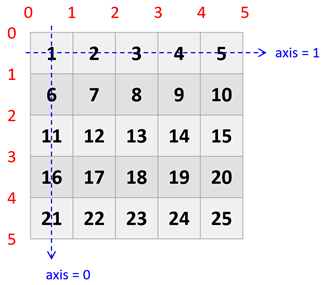
\includegraphics[width=300]{images/aryaxis.jpg}
\caption{\label{fig:ndaryAix}Axis in ndarray}
\end{figure}
\item 其他常用函數
\label{sec:org0c619b9}
\begin{itemize}
\item min()\\
\item max()\\
\item mean()\\
\item std()\\
\item var()\\
\item sqrt()\\
\end{itemize}

\lstset{breaklines=true,language=Python,label= ,caption= ,captionpos=b,firstnumber=1,numbers=left}
\begin{lstlisting}
import numpy as np

np1 = np.random.randint(0, 10, size=[3, 2])
print("np\n", np1)
print("np1.sum", np1.sum())
print("sum:", sum(np1))
print("sum:", sum(np1,3))
print("min:", np1.min())
print("max:", np1.max())
print("mean:", np.mean(np1))
\end{lstlisting}

\begin{verbatim}
np
 [[3 1]
 [2 1]
 [8 9]]
np1.sum 24
sum: [13 11]
sum: [16 14]
min: 1
max: 9
mean: 4.0
\end{verbatim}
\item sum() v.s. np.sum()
\label{sec:orgddcc3bc}
\begin{figure}[htbp]
\centering
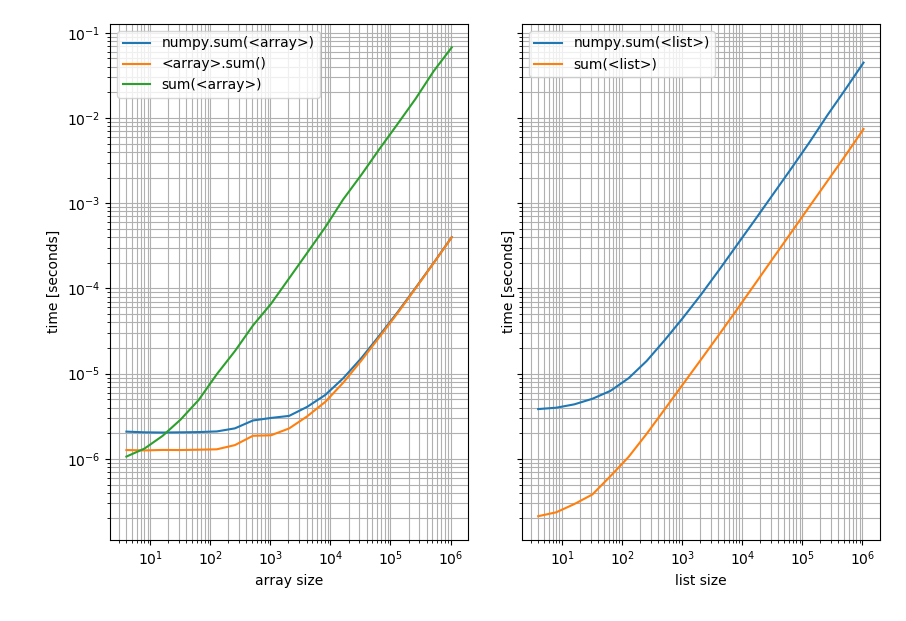
\includegraphics[width=400]{images/2sum.png}
\caption{\label{fig:SimpleSin}sum() v.s. np.sum()}
\end{figure}
\end{enumerate}
\subsection{實作練習}
\label{sec:org4dfc599}
\begin{enumerate}
\item 練習要求
\label{sec:org128c3f6}
\begin{enumerate}
\item 隨機產生一組 150 個 0\textasciitilde{}100 的陣列。\\
\item 將上述陣列 reshape 為 30*5 的二維陣列，模擬成一個班級的某次考試成績(30 人*5 科)。\\
\item 輸出此次 5 科考科的全班總分、平均。某班資電腦科期中考成績(30 人，分數為 0\textasciitilde{}100)，將分數以「開根\\
號乘以 10」的方式修正，求全班最高分、最低分、平均。\\
\item 輸出各科標準差(提示：std)\\
\item 將全班分數以「開根號乘以 10」的方式進行調整。\\
\item 上述輸出至小數點第二位(提示：set\_printoptions)\\
\end{enumerate}
\item 結果範例
\label{sec:org7622395}
\begin{verbatim}
各科總分: [1427 1338 1417 1380 1678]
各科平均: [47.57 44.6  47.23 46.   55.93]
各科最高分: [97 95 98 96 99]
各科最低分: [2 0 0 6 0]
各科標準差: [31.56 30.23 31.07 30.47 32.93]
調整分數:
 [[96.95 68.56 24.49 36.06 81.24]
 [75.5  20.   55.68 97.98 92.74]
 [20.   70.   60.   94.34 91.65]
 [41.23 56.57 91.1  55.68 97.47]
 [98.49 43.59  0.   36.06 71.41]
 [52.92 41.23 95.92 83.07 53.85]
 [97.98 94.34 52.92 50.   93.81]
 [47.96 74.83 54.77 50.   22.36]
 [81.85 63.25 90.   68.56 97.47]
 [67.82 66.33 82.46 86.02 91.65]
 [81.85 75.5  46.9  66.33 40.  ]
 [45.83 80.62 56.57 30.   87.18]
 [50.99 97.47 98.99 93.81 99.5 ]
 [98.49 95.39 88.88 24.49 91.65]
 [60.   73.48 90.55 24.49 74.16]
 [50.   93.27 89.44 91.65 99.5 ]
 [77.46 28.28 34.64 24.49 28.28]
 [91.65 46.9  72.11 97.98 57.45]
 [60.83 87.75 68.56 75.5  61.64]
 [93.81 24.49 84.85 36.06 96.95]
 [69.28 55.68 83.67 36.06 95.39]
 [96.44 86.6  17.32 76.16 60.  ]
 [77.46 83.67 37.42 96.95  0.  ]
 [31.62 14.14 76.16 67.08 61.64]
 [64.81 30.   36.06 84.26 87.75]
 [40.   26.46 97.98 40.   10.  ]
 [31.62 95.92 85.44 82.46 76.16]
 [14.14  0.   58.31 54.77 74.83]
 [85.44 67.08 33.17 68.56 44.72]
 [17.32 69.28 37.42 68.56 40.  ]]
\end{verbatim}

\newpage
\end{enumerate}

\section{Matplotlib}
\label{sec:orgc25aa14}
\subsection{Matplotlib 簡介}
\label{sec:org51066fc}
\begin{itemize}
\item Matplotlib 是利用 Python 所實作的繪圖套件，其中包含兩個最重要的模組: pylab 和\\
pyplot。\\
\item pylab 已經幾乎實作了在學術介最常用的套件 — Matlab 所支援的繪圖功能，或\\
者可以說 pylab 其實就是 Matlab 的 Python 版本；\\
\item pyplot 是把 pylab 再加上 Numpy，讓使用者在使用 pyplot 時，可以直\\
接呼叫 Numpy 的函式做計算後再以圖型的方式呈現。\footnote{\href{https://medium.com/@jemmy1234/matplotlib-\%E7\%B0\%A1\%E4\%BB\%8B-857323964e2d}{Matplotlib 簡介}\\}\\
\item 為 Python 最多人使用的 2D 繪圖工具\\
\item 優點：圖形美觀、類型多、相容於 Matlab\\
\item 官方社群網站 \url{https://matplotlib.org/}\\
\item 維基百科 \url{https://zh.wikipedia.org/wiki/Matplotlib}\\
\end{itemize}
\subsection{Matplotlib 基本語法}
\label{sec:org8d55638}
\begin{enumerate}
\item 基本語法
\label{sec:orgcbe67db}
\begin{itemize}
\item import matplotlib.pyplot as plt\\
\item \href{https://matplotlib.org/3.2.1/api/\_as\_gen/matplotlib.pyplot.plot.html}{plt.plot()函式}為 matplotlib.pyplot 模組畫線條方法，其語法如下
\\
\end{itemize}
\lstset{breaklines=true,language=Python,label= ,caption= ,captionpos=b,numbers=none}
\begin{lstlisting}
plt.plot( [x座標資料,] y座標資料 [, 參數1, 參數2, ...] )
\end{lstlisting}
\item 範例:簡單的 sin 圖形
\label{sec:org4dade57}
\begin{itemize}
\item np.sin( )函式為 Numpy 模組求正弦值\\
\item plt.show( )函式用來顯示圖形\\
\end{itemize}
\lstset{breaklines=true,language=Python,label= ,caption= ,captionpos=b,firstnumber=1,numbers=left}
\begin{lstlisting}
import matplotlib.pyplot as plt
import numpy as np

x = np.arange(-3, 3, 0.1)
plt.clf()
plt.plot(x, np.sin(x))

# 若要存圖，要先存檔再顯示 # for jupyter
plt.savefig('images/SimpleSin.png', dpi=300)
# plt.show()   # for jupyter


\end{lstlisting}
\begin{figure}[htbp]
\centering
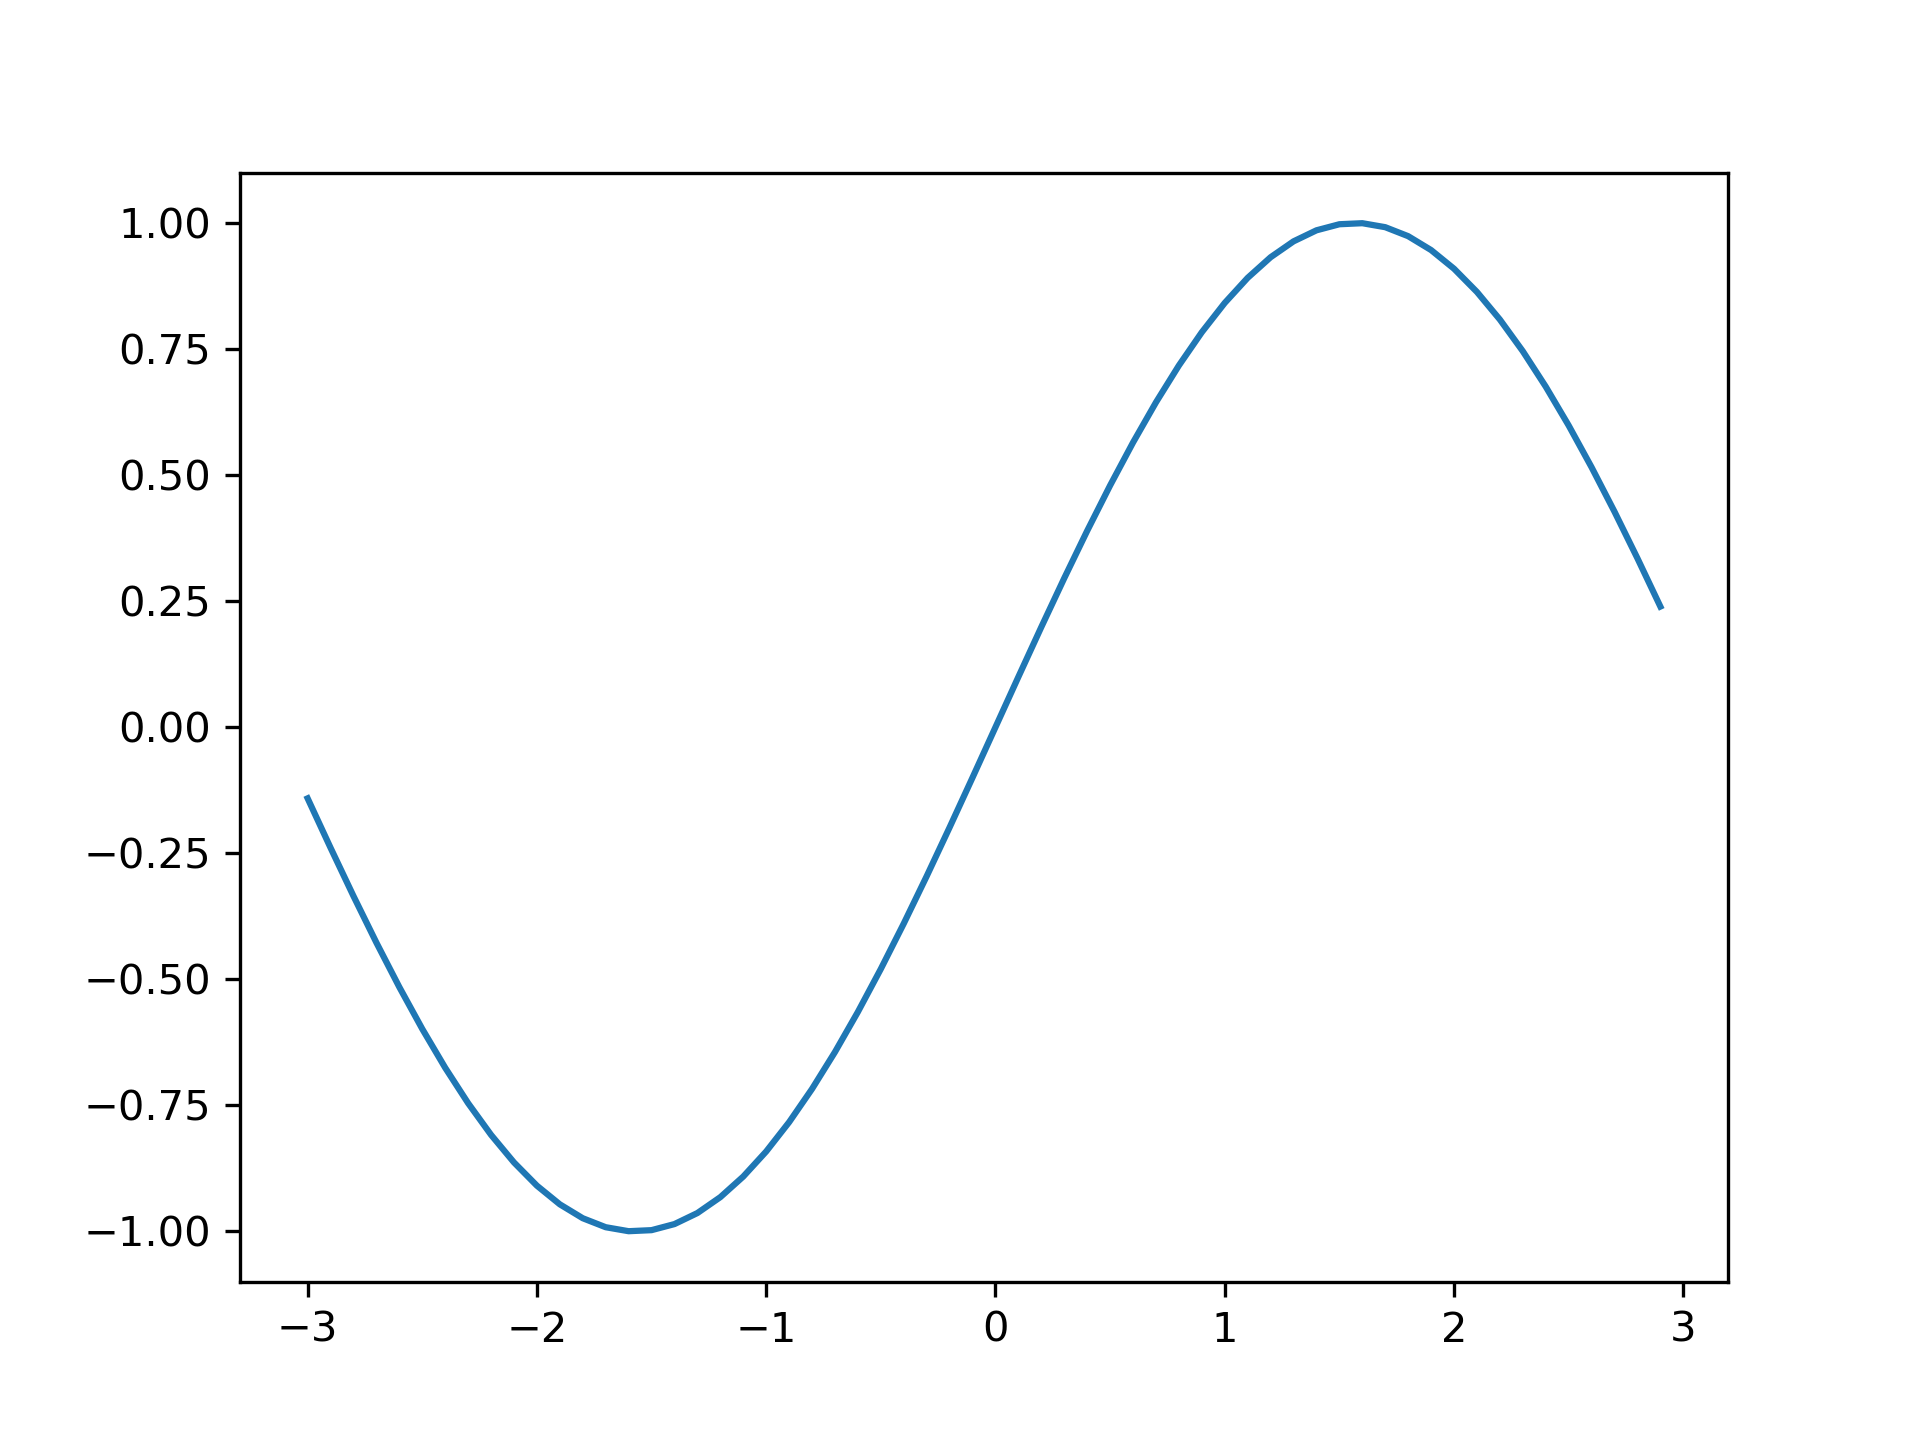
\includegraphics[width=300]{images/simpleSin.png}
\caption{\label{fig:SimpleSin}簡單的 sin 圖形}
\end{figure}
\item plot 官方語法
\label{sec:orgf043fcd}
\begin{itemize}
\item plot([x], y, [fmt], *, data=None, **kwargs)\\
\item plot([x], y, [fmt], [x2], y2, [fmt2], \ldots{}, **kwargs)\\
\end{itemize}
\item plot()函式兩類參數：fmt 字串、 kwarg 參數
\label{sec:org7e02344}
\begin{enumerate}
\item fmt
\label{sec:org82edf13}
\begin{itemize}
\item 可選引數 fmt 是定義基本格式 (如顏色、標記和 linestyle) 的簡便方法\\
\item plot(): fmt 字串\\
\end{itemize}
\begin{center}
\begin{tabular}{llllll}
字元 & 顏色 & 字元 & 標記 & 字元 & 標記\\
\hline
'b' & 藍 & '.' & 點 & '*' & *\\
'g' & 綠 & 'o' & 圓圈 & '+' & +\\
'r' & 紅 & 'v' & 三角形(下) & 'x' & x\\
'c' & 青 & '\^{}' & 三角形(上) & 'd' & 鑽石\\
'm' & 洋紅 & '<' & 三角形(左) & 字元 & 線條\\
'y' & 黃 & '>' & 三角形(右) & '-' & 實線\\
'k' & 黑 & 's' & 正方形 & '--' & 虛線\\
'w' & 白 & 'p' & 五邊形 & '-.' & -.-.-.-.\\
\end{tabular}
\end{center}
\lstset{breaklines=true,language=Python,label= ,caption= ,captionpos=b,firstnumber=1,numbers=left}
\begin{lstlisting}
import matplotlib.pyplot as plt
import numpy as np

x = np.arange(-3, 3, 0.1)
plt.clf()
plt.plot(x, np.sin(x), 'r+')
# for web-based
# plt.show()

# saving figure
plt.savefig('SimpleSin2.png', dpi=300)

\end{lstlisting}
\begin{figure}[htbp]
\centering
\includegraphics[width=300]{simpleSin2.png}
\caption{\label{fig:SimpleSin}簡單的 sin 圖形}
\end{figure}
\begin{itemize}
\item 多組資料\\
\end{itemize}
\lstset{breaklines=true,language=Python,label= ,caption= ,captionpos=b,firstnumber=1,numbers=left}
\begin{lstlisting}
import matplotlib.pyplot as plt
import numpy as np

x1 = np.arange(-3, +3, 0.1)
y1 = np.sin(x1)
y2 = np.cos(x1)

#plt.plot(x1, y1, 'r^--', x1, y2, 'go-')
plt.plot(x1, y1, 'r^--', x1, y2, 'go-')
plt.savefig('mline.png', dpi=300)

\end{lstlisting}
\begin{figure}[htbp]
\centering
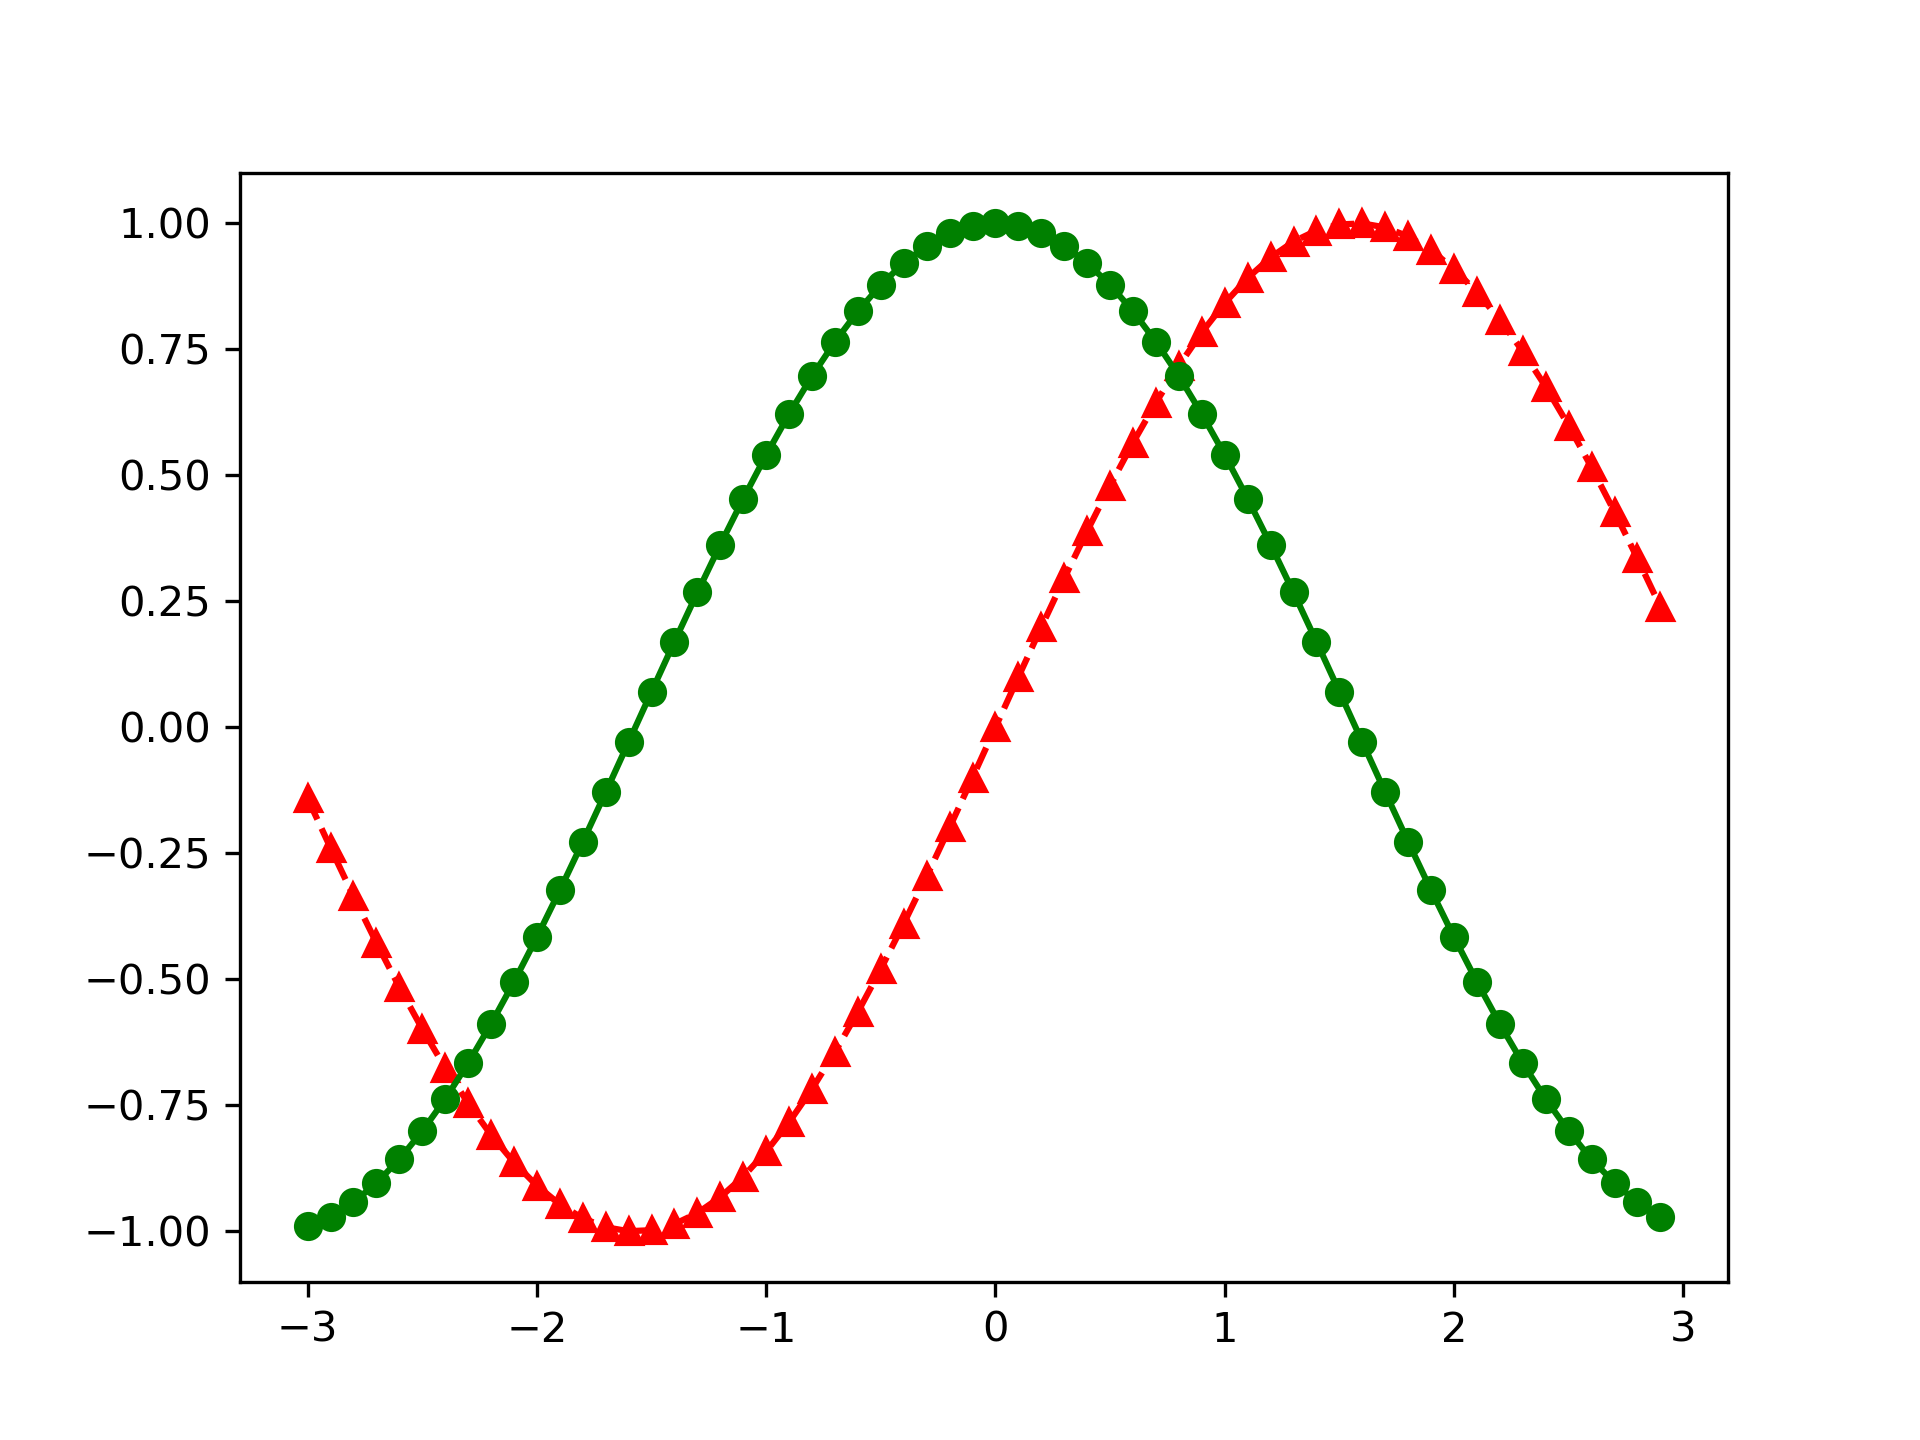
\includegraphics[width=300]{mline.png}
\caption{\label{fig:multi-line}多組圖形}
\end{figure}
\item kwgarg 參數
\label{sec:org18c172b}
\begin{enumerate}
\item kwarg 為 Line2D 屬性：\href{https://matplotlib.org/3.1.0/gallery/color/named\_colors.html}{color}, linestyle, marker, label, linewidth, ….
\label{sec:org6be5fd7}
\begin{itemize}
\item kwargs 用於指定諸如線條標籤 (用於自動圖例)、線寬、抗鋸齒、標記面顏色等屬性\\
\item 若 fmt 和 kwarg 設定衝突時，以 kwarg 為主\\
\end{itemize}
\item color
\label{sec:org8b9ab91}
\begin{itemize}
\item 單字，如 g：color = 'lime'\\
\item 字母，如 g：color = 'k'\\
\item 色碼，如 g：color = '\#FF0000'\\
\item RGB 值(0\textasciitilde{}g1 之間)，如：color = (1, 0, 0)\\
\end{itemize}
\begin{center}
\begin{tabular}{ll}
字元 & 顏色\\
\hline
'b' & 藍色\\
'g' & 綠色\\
'r' & 紅\\
'c' & 青色\\
'm' & 品紅\\
'y' & 黃色\\
'k' & 黑\\
'w' & 白色\\
\end{tabular}
\end{center}
\item marker
\label{sec:org0f7c22f}
\begin{center}
\begin{tabular}{ll}
字元 & 描述\\
\hline
'.' & 點標記\\
',' & 畫素標記\\
'o' & 圓圈標記\\
'v' & triangle\_down 標記\\
'\^{}' & triangle\_up 標記\\
'<' & triangle\_left 標記\\
'>' & triangle\_right 標記\\
'1' & tri\_down 標記\\
'2' & tri\_up 標記\\
'3' & tri\_left 標記\\
'4' & tri\_right 標記\\
's' & 方形標記\\
'p' & 五角大樓標記\\
'*' & 星形標記\\
'h' & hexagon1 標記\\
'H' & hexagon2 標記\\
'+' & 加號標記\\
'x' & x 標記\\
'D' & 鑽石標記\\
'd' & thin\_diamond 標記\\
'\(\vert{}\)' & 圴標記\\
'\_' & 修身標記\\
\end{tabular}
\end{center}
\item linestyle
\label{sec:org3b2397d}
\begin{center}
\begin{tabular}{ll}
字元 & 描述\\
\hline
'-' & 實線樣式\\
'--' & 虛線樣式\\
'-.' & 破折號-點線樣式\\
':' & 虛線樣式\\
\end{tabular}
\end{center}
\item label
\label{sec:org1fbd49c}
\begin{itemize}
\item fg 呈現線條標籤，如 label = 'y = x\textsuperscript{2}'\\
\item 需搭配 pglt.legend()函式方能呈現 label\\
\end{itemize}
\end{enumerate}
\item 其他參數
\label{sec:org57b7589}
\begin{itemize}
\item x / y 座標範圍：plt.xlim(起始值, 終止值)  / plt.ylim(起, 止)\\
\item 圖表標題：plt.title(字串)\\
\item x / y 座標標題：plt.xlabel(字串) / plt.ylabel(字串)\\
\item 顯示 kwarg 參數裡的 label：plt.legend()\\
\end{itemize}
\item kwarg 示範
\label{sec:org5e42d67}
\lstset{breaklines=true,language=Python,label= ,caption= ,captionpos=b,firstnumber=1,numbers=left}
\begin{lstlisting}
import matplotlib.pyplot as plt
import numpy as np

x = np.arange(-3, 3, 0.5)
plt.clf()
plt.plot(x, np.cos(x), color='c', linestyle='--', marker='p')
plt.xlim(-4, 4)
plt.xlabel('This is x label')
plt.title("This is Title", fontsize=16)

plt.savefig('images/kwarg.png', dpi=300)

\end{lstlisting}
\begin{figure}[htbp]
\centering
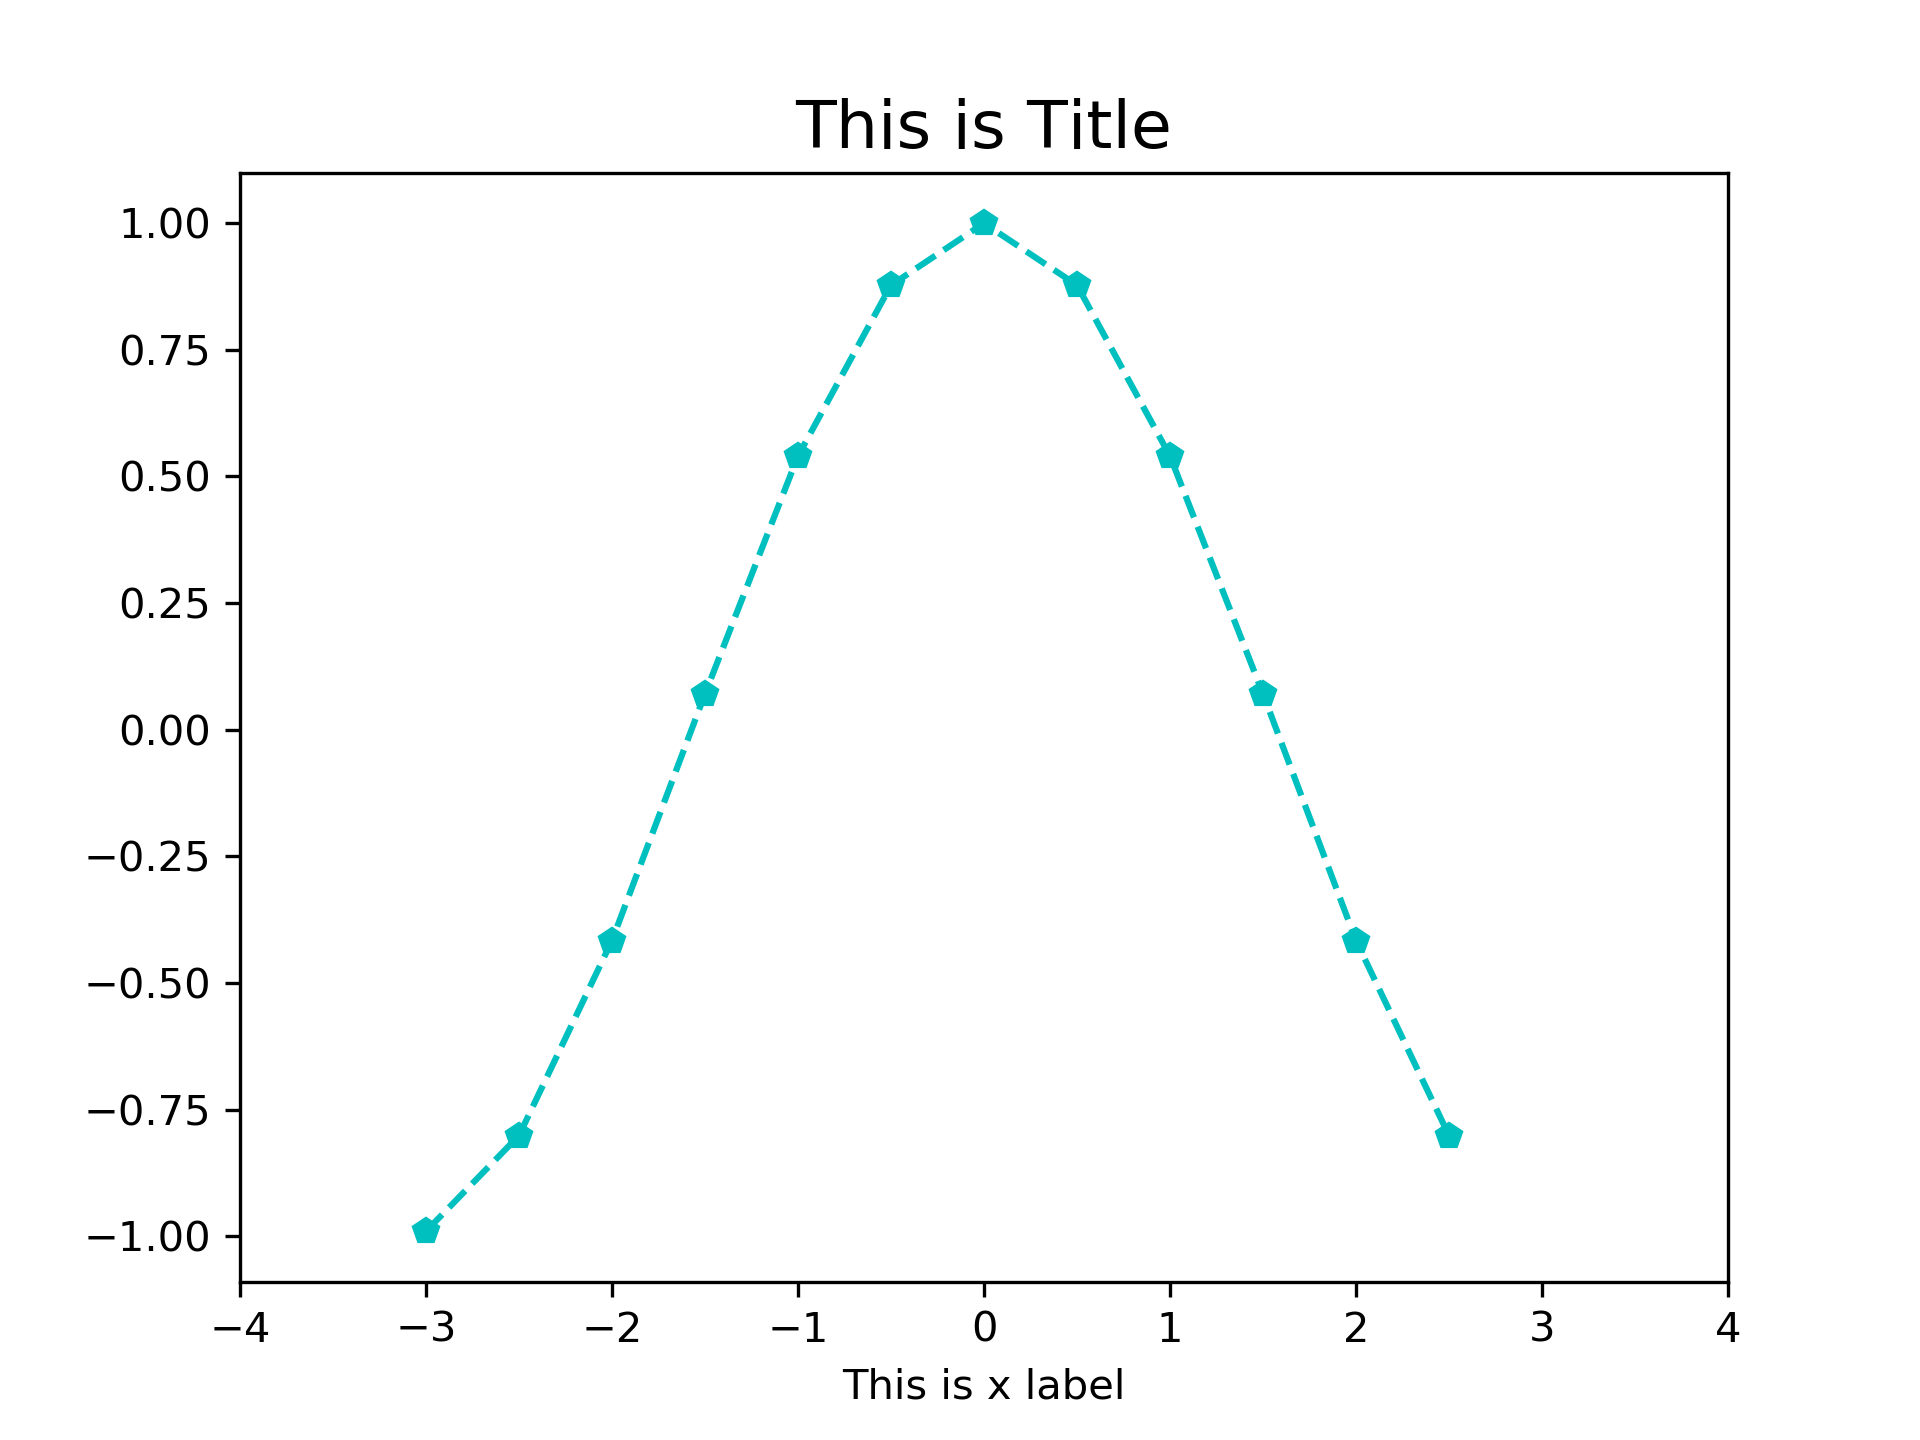
\includegraphics[width=400]{images/kwarg.png}
\caption{\label{fig:kwarg}多組線圖}
\end{figure}
\item 中文問題
\label{sec:org5301adb}
\begin{itemize}
\item 解決方案\\
\end{itemize}
\lstset{breaklines=true,language=Python,label= ,caption= ,captionpos=b,firstnumber=1,numbers=left}
\begin{lstlisting}
# 解決中文問題
plt.rcParams['font.sans-serif'] = ['SimHei'] # 步驟一（替換sans-serif字型）
plt.rcParams['axes.unicode_minus'] = False  # 步驟二（解決座標軸負數的負號顯示問題）
\end{lstlisting}

\begin{itemize}
\item 實際示例\\
\end{itemize}
\end{enumerate}
\end{enumerate}
\subsection{Line Chart}
\label{sec:org61a7e4b}
\begin{enumerate}
\item 折線示範\#1
\label{sec:org56fce35}
\lstset{breaklines=true,language=Python,label= ,caption= ,captionpos=b,firstnumber=1,numbers=left}
\begin{lstlisting}
import matplotlib.pyplot as plt
import numpy as np

x1 = [1, 2, 3, 4, 5, 6]
y1 = [1, 2, 3, 4, 5, 6]
x2 = np.arange(0, 3, 0.3)
x3 = np.arange(8).reshape(2, 4)
print(x3)
print(x3+3)
plt.plot(y1, 'c-p', x2, x2**2, 'ms:', x3, x3+3, '-*')
plt.savefig('line2.png', dpi=300)
\end{lstlisting}
\begin{verbatim}
[[0 1 2 3]
 [4 5 6 7]]
[[ 3  4  5  6]
 [ 7  8  9 10]]
\end{verbatim}

\begin{figure}[htbp]
\centering

\includegraphics[width=400]{line2.png}
\caption{\label{fig:SimpleSin}簡單的折線圖形 2}
\end{figure}

\item 練習
\label{sec:orgc4363e9}
\begin{enumerate}
\item \label{練習#1}：繪製折線圖
\label{sec:org8c2dc84}
\begin{itemize}
\item 利用 list 繪製
\\
\begin{itemize}
\item x1 = [1, 2, 3, 4, 5, 6]
\\
\item y1 = [1, 2, 3, 4, 5, 6]
\\
\end{itemize}
\item 執行 plt.plot(y1) 和 plt.plot(x1, y1) 有何差別??\\
\item 利用 numpy 繪製
\\
\begin{itemize}
\item x2 = np.arange(0, 3, 0.01)
\\
\end{itemize}
\item 執行 plt.plot(x2, x2**2)看看畫出什麼圖形??\\
\end{itemize}
\end{enumerate}
\end{enumerate}
\subsection{Bar chart}
\label{sec:orge597bf5}
\begin{itemize}
\item 語法\\
\end{itemize}
\lstset{breaklines=true,language=Python,label= ,caption= ,captionpos=b,numbers=none}
\begin{lstlisting}
plt.bar( x座標資料, y座標資料 [, 參數1, 參數2, ...] )
plt.barh( x座標資料, y座標資料 [, 參數1, 參數2, ...] )
\end{lstlisting}
\begin{itemize}
\item DEMO\\
\end{itemize}
\lstset{breaklines=true,language=Python,label= ,caption= ,captionpos=b,firstnumber=1,numbers=left}
\begin{lstlisting}
import matplotlib.pyplot as plt
import numpy as np

objects = ('Python', 'C++', 'Java', 'Perl', 'Scala', 'Lisp')
y_pos = np.arange(len(objects))
performance = [10,8,6,4,2,1]

plt.barh(y_pos, performance, align='center', color = ['b','g','r','c','m','y'], alpha=0.5)
plt.yticks(y_pos, objects)
plt.xlabel('Usage')
plt.title('Programming language usage')
#plt.show()
plt.savefig('barChart.png', dpi=300)

\end{lstlisting}
\begin{figure}[htbp]
\centering
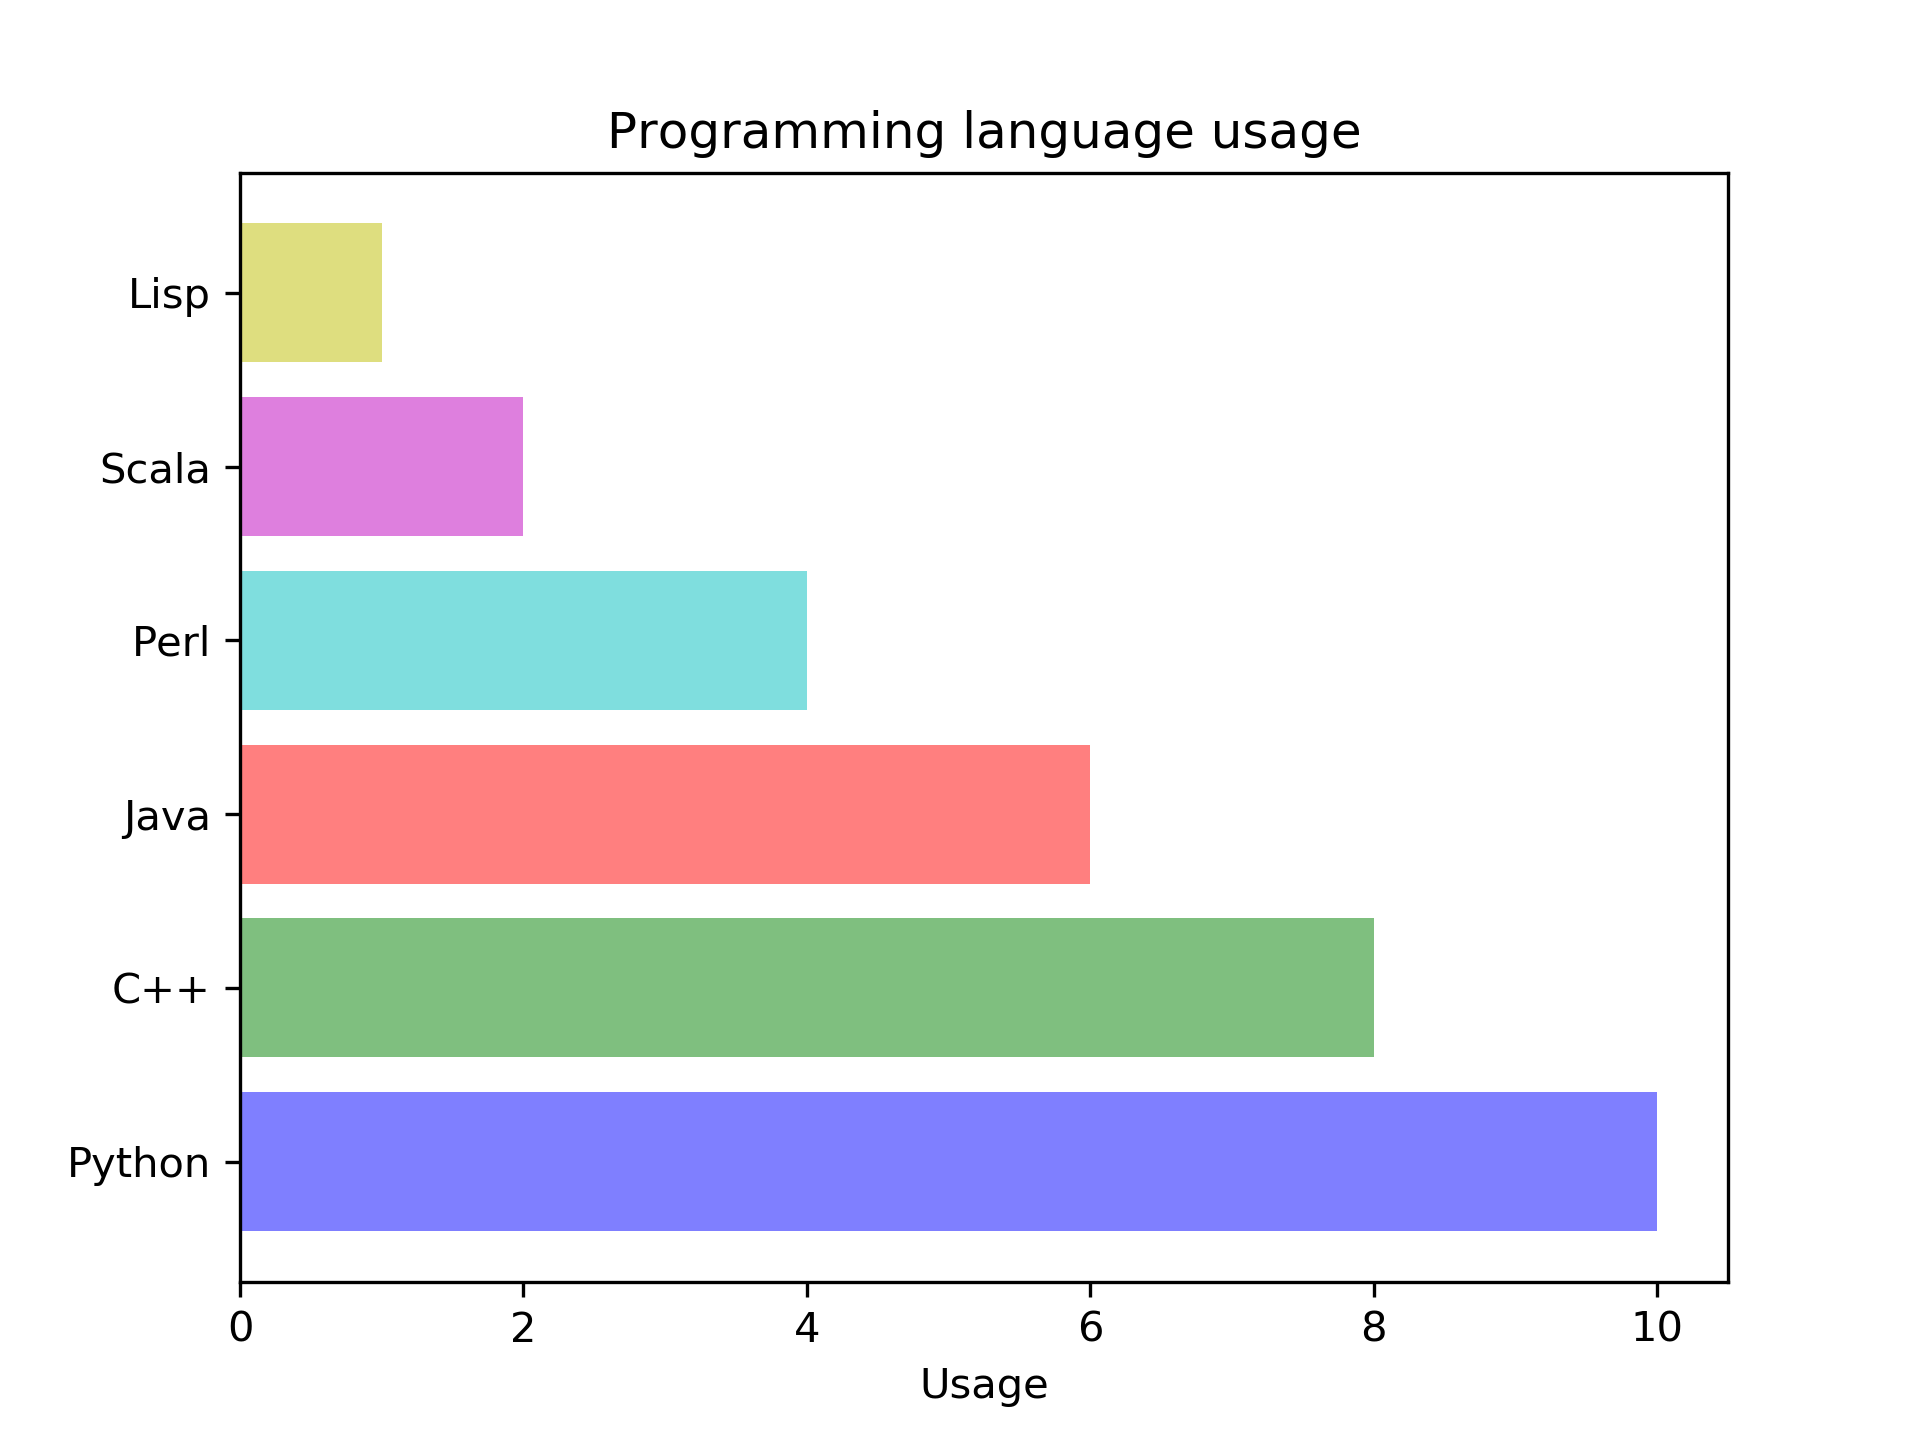
\includegraphics[width=300]{barChart.png}
\caption{\label{fig:barChart}barChart Demo}
\end{figure}

\subsection{Pie chart}
\label{sec:org9b8c72c}
\begin{enumerate}
\item 語法：

\label{sec:orgaa0db91}
plt.pie( 比例列表 [, 參數 1, 參數 2, \ldots{}] )\\
\item 參數：
\label{sec:orgf05113c}
\begin{itemize}
\item colors：各子圖顏色，多以 list 表示\\
\item labels：各子圖標籤，多以 list 表示\\
\item explode：各子圖分離突出比例，0.1 代表分離 10\%，多以 list 表示\\
\item autopct：顯示各子圖比例值，格式為\%x.y\%\%\\
\item startangle：繪製起始角度，預設為 0 (與三角函數角度相同)\\
\item 若要以正圓形繪製，請再加上 \href{https://matplotlib.org/3.2.1/api/\_as\_gen/matplotlib.pyplot.axis.html}{plt.axis}('equal')\\
\item legend location\\
\end{itemize}
\begin{center}
\begin{tabular}{lr}
Location String & Location Code\\
\hline
'best' & 0\\
'upper right' & 1\\
'upper left' & 2\\
'lower left' & 3\\
'lower right' & 4\\
'right' & 5\\
'center left' & 6\\
'center right' & 7\\
'lower center' & 8\\
'upper center' & 9\\
'center' & 10\\
\end{tabular}
\end{center}
\item 範例
\label{sec:org7ec3337}
\lstset{breaklines=true,language=Python,label= ,caption= ,captionpos=b,firstnumber=1,numbers=left}
\begin{lstlisting}
import matplotlib.pyplot as plt
import numpy as np

parts = [35.35, 23, 26.65, 15]
labels = ['Harrison', 'Vanessa', 'James', 'Ruby']
colors = ['red', 'lightblue', 'purple', 'yellow']
explodes = [0.1, 0, 0, 0.1]
plt.pie(parts, colors = colors, labels = labels, explode = explodes, autopct = '%3.2f%%')
plt.axis('equal')
plt.legend(loc='upper left')

#plt.show()
plt.savefig('simplePie.png', dpi=300)
\end{lstlisting}
\begin{figure}[htbp]
\centering

\includegraphics[width=300]{simplePie.png}
\caption{\label{fig:SimplePie}簡單的 pie chart}
\end{figure}
\end{enumerate}
\subsection{其它圖表}
\label{sec:org77eaf87}
\begin{itemize}
\item 直方圖(Histogram)：用來呈現各資料統計結果(\href{https://matplotlib.org/api/\_as\_gen/matplotlib.pyplot.hist.html}{參考資料})\\
\item 散佈圖(Scatter)：用來呈現群聚關係(\href{https://matplotlib.org/api/\_as\_gen/matplotlib.pyplot.scatter.html}{參考資料})\\
\item \href{https://matplotlib.org/gallery/index.html}{進階學習資源}\\
\end{itemize}
\subsection{文字註解: plt.text()}
\label{sec:orgaea640f}
\begin{enumerate}
\item 語法
\label{sec:orgbccb856}
\begin{itemize}
\item \lstinline[breaklines=true,language=Python]~ plt.text( x相對座標, y相對座標 , 文字字串 [, 其它參數] ) ~\\
\item \href{https://matplotlib.org/api/\_as\_gen/matplotlib.pyplot.text.html}{參考資料}\\
\end{itemize}
\item 範例
\label{sec:orgd49bde1}
\lstset{breaklines=true,language=Python,label= ,caption= ,captionpos=b,firstnumber=1,numbers=left}
\begin{lstlisting}
import matplotlib.pyplot as plt

x = [1, 2, 3, 4, 5, 6, 7, 8]
y = [1, 4, 9, 16, 25, 36, 49, 64]
plt.plot(x, y, 'r--')
for x, y in zip(x, y):
    plt.text(x-0.2, y+0.6, '(%d, %d)' %(x, y))
#plt.show()
plt.savefig('simpleText.png', dpi = 300)
\end{lstlisting}

\begin{figure}[htbp]
\centering
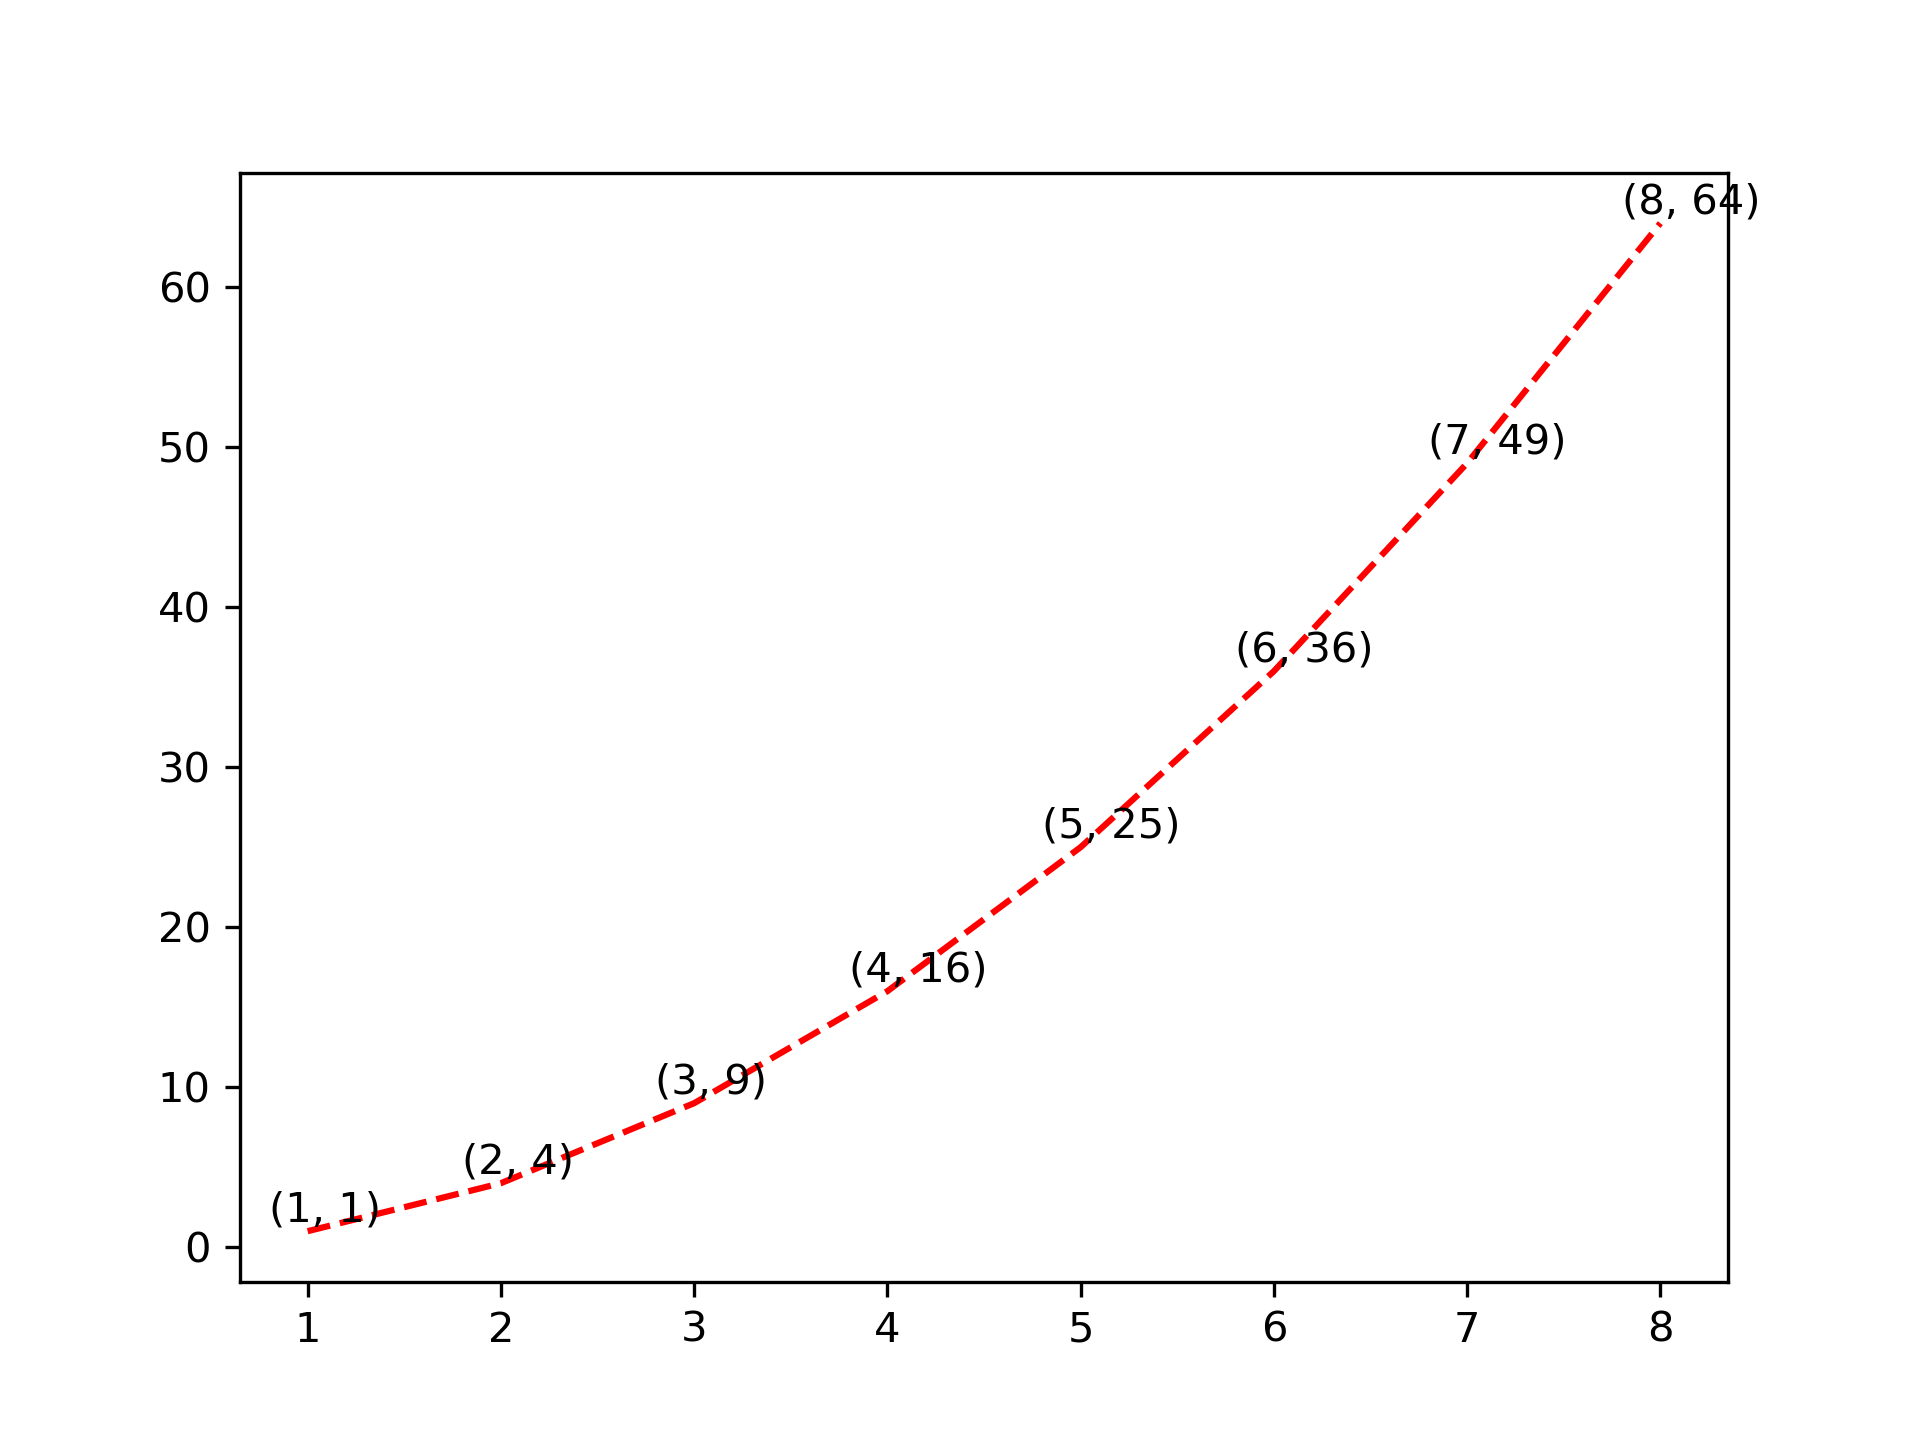
\includegraphics[width=300]{simpleText.png}
\caption{\label{fig:SimplePie}簡單的文字註解}
\end{figure}
\end{enumerate}
\subsection{子圖表: plt.subplot()}
\label{sec:org09a471a}
\begin{enumerate}
\item 範例\footnote{\href{https://matplotlib.org/api/\_as\_gen/matplotlib.pyplot.subplot.html}{matplotlib.pyplot.subplot}\\}
\label{sec:orgef7cce7}
\lstset{breaklines=true,language=Python,label= ,caption= ,captionpos=b,firstnumber=1,numbers=left}
\begin{lstlisting}
import numpy as np
import matplotlib.pyplot as plt

from matplotlib.ticker import NullFormatter  # useful for `logit` scale

# Fixing random state for reproducibility
np.random.seed(19680801)

# make up some data in the interval ]0, 1[
y = np.random.normal(loc=0.5, scale=0.4, size=1000)
y = y[(y > 0) & (y < 1)]
y.sort()
x = np.arange(len(y))

# plot with various axes scales
plt.figure()

# linear
plt.subplot(221)
plt.plot(x, y)
plt.yscale('linear')
plt.title('linear')
plt.grid(True)


# log
plt.subplot(222)
plt.plot(x, y)
plt.yscale('log')
plt.title('log')
plt.grid(True)


# symmetric log
plt.subplot(223)
plt.plot(x, y - y.mean())
plt.yscale('symlog', linthreshy=0.01)
plt.title('symlog')
plt.grid(True)

# logit
plt.subplot(224)
plt.plot(x, y)
plt.yscale('logit')
plt.title('logit')
plt.grid(True)
# Format the minor tick labels of the y-axis into empty strings with
# `NullFormatter`, to avoid cumbering the axis with too many labels.
plt.gca().yaxis.set_minor_formatter(NullFormatter())
# Adjust the subplot layout, because the logit one may take more space
# than usual, due to y-tick labels like "1 - 10^{-3}"
plt.subplots_adjust(top=0.92, bottom=0.08, left=0.10, right=0.95, hspace=0.25, wspace=0.35)

plt.savefig('simpleSubplot.png', dpi = 300)
\end{lstlisting}

\begin{figure}[htbp]
\centering
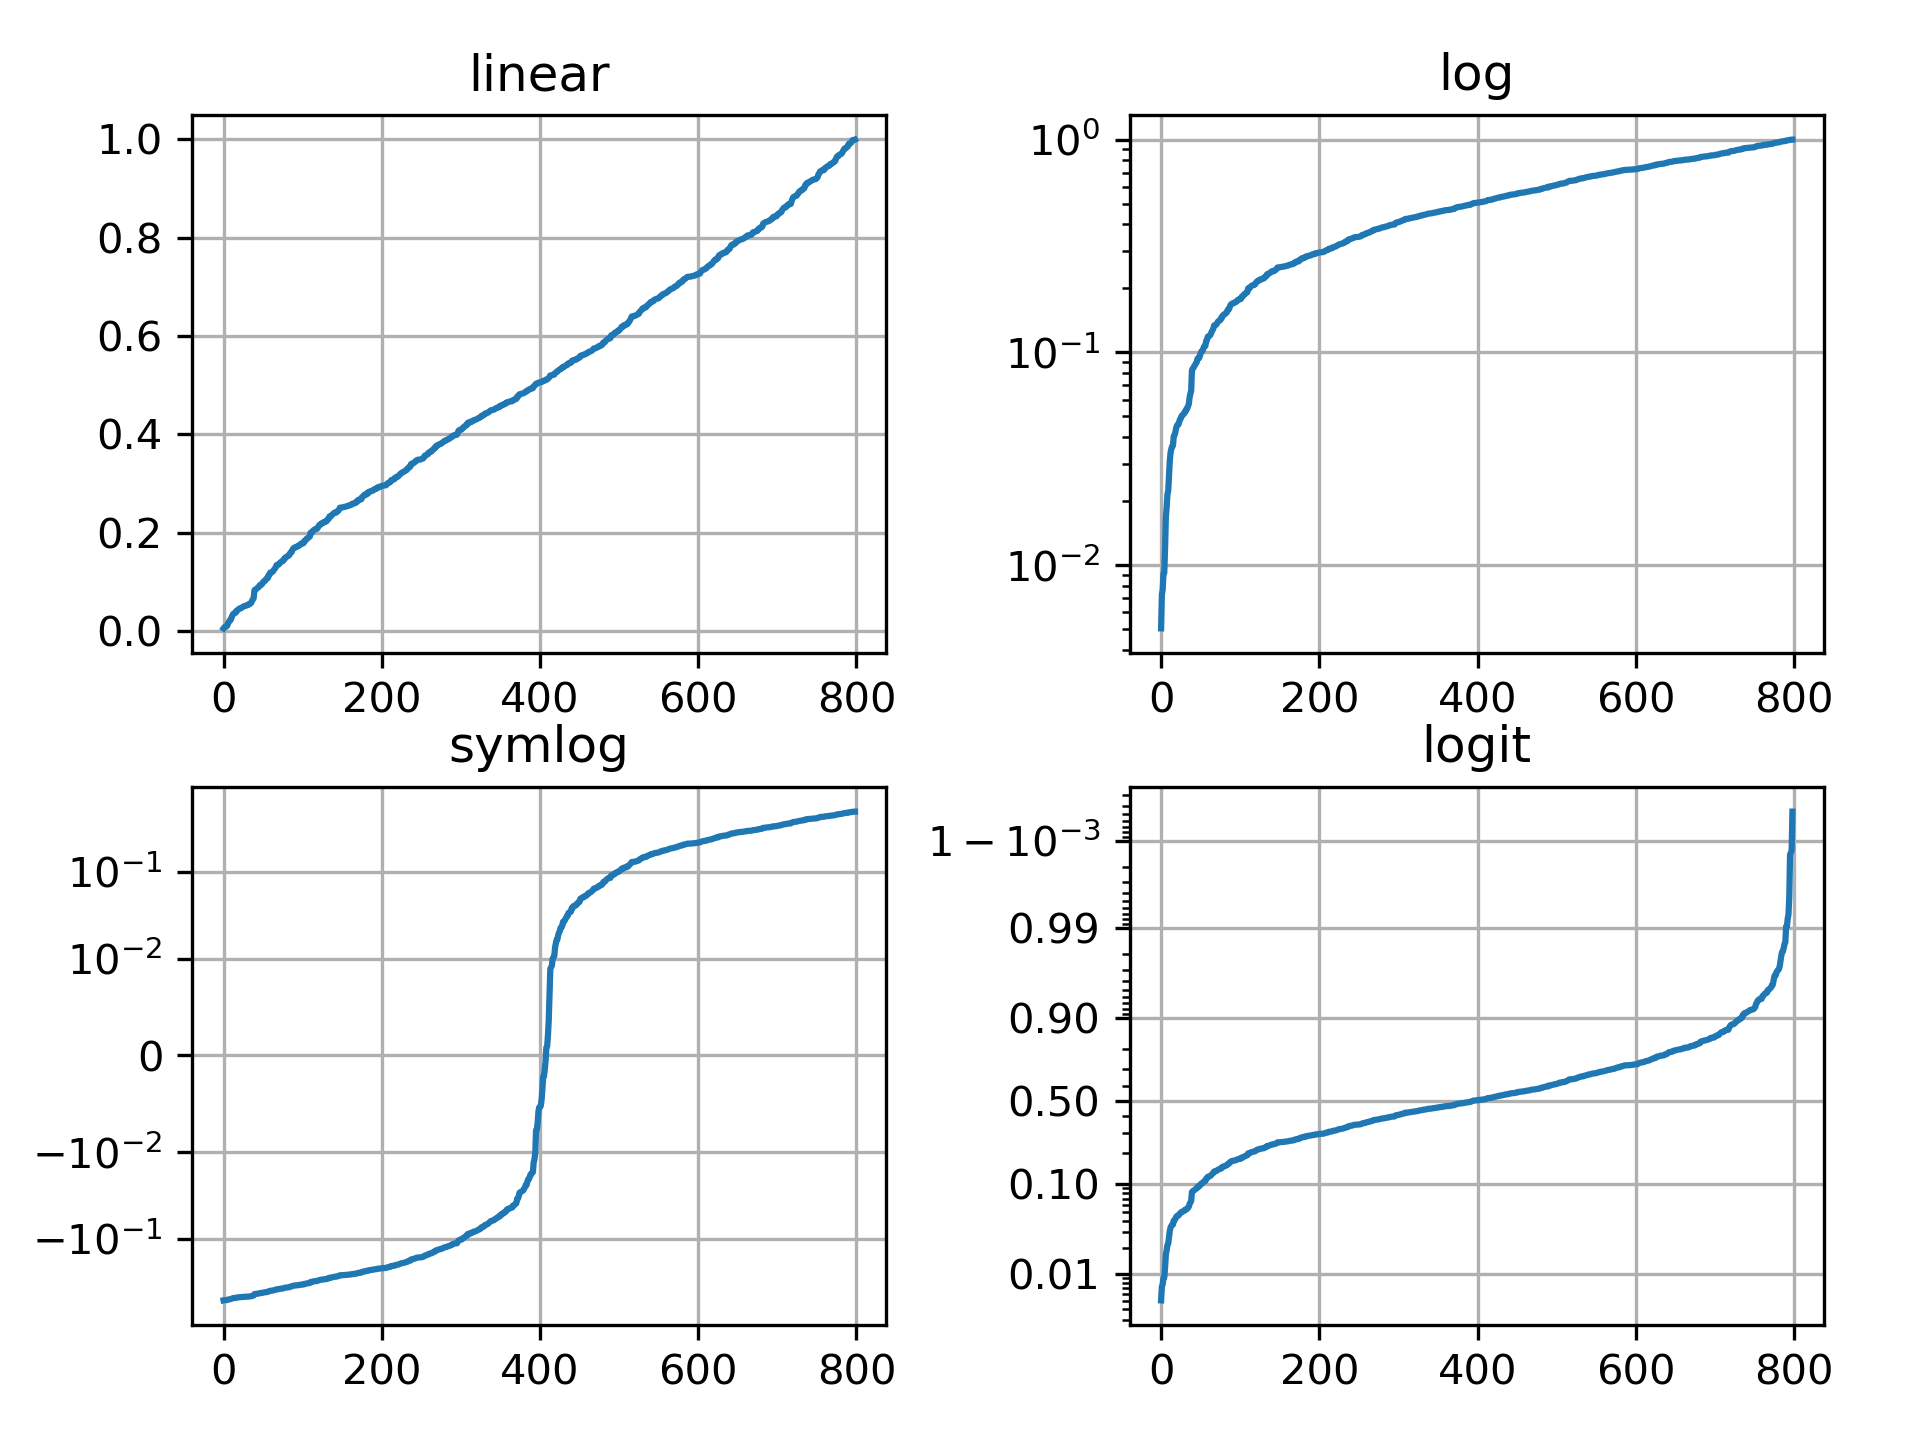
\includegraphics[width=400]{simpleSubplot.png}
\caption{\label{fig:SimpleSubplot}簡單的子圖表}
\end{figure}

\item 進階設定
\label{sec:orgb7f7e3b}
\begin{itemize}
\item \href{https://matplotlib.org/api/\_as\_gen/matplotlib.pyplot.subplot.html}{官網}\\
\item \href{https://ithelp.ithome.com.tw/articles/10201670}{視覺化資料 - Matplotlib - legend、subplot、GridSpec、annotate}\\
\item \href{https://www.delftstack.com/zh-tw/howto/matplotlib/how-to-make-different-subplot-sizes-in-matplotlib/}{Matplotlib 中如何建立不同大小的子圖 subplot}\\
\end{itemize}
\end{enumerate}
\subsection{實作練習}
\label{sec:org86174c2}
\begin{enumerate}
\item 輸入 a, b, c，畫出曲線圖：y=\(ax^2+bx+c\)
\label{sec:org9624765}
\item 將前一章的練習題所產生 30*5 的二維隨機陣列，將五科科目的平均製成長條圖，此五科科目設定為:國文、英文、數學、理化、史地。
\label{sec:org433fc57}
\item 找出國文與英文兩科成績，畫出兩科成績的散佈圖(Scatter)，觀察學生在這兩科的得分是否有正相關。
\label{sec:org51b97f8}

\item 參考解答
\label{sec:orgd6faaaf}
\begin{enumerate}
\item \#1
\label{sec:org9ca50a2}
\begin{figure}[htbp]
\centering
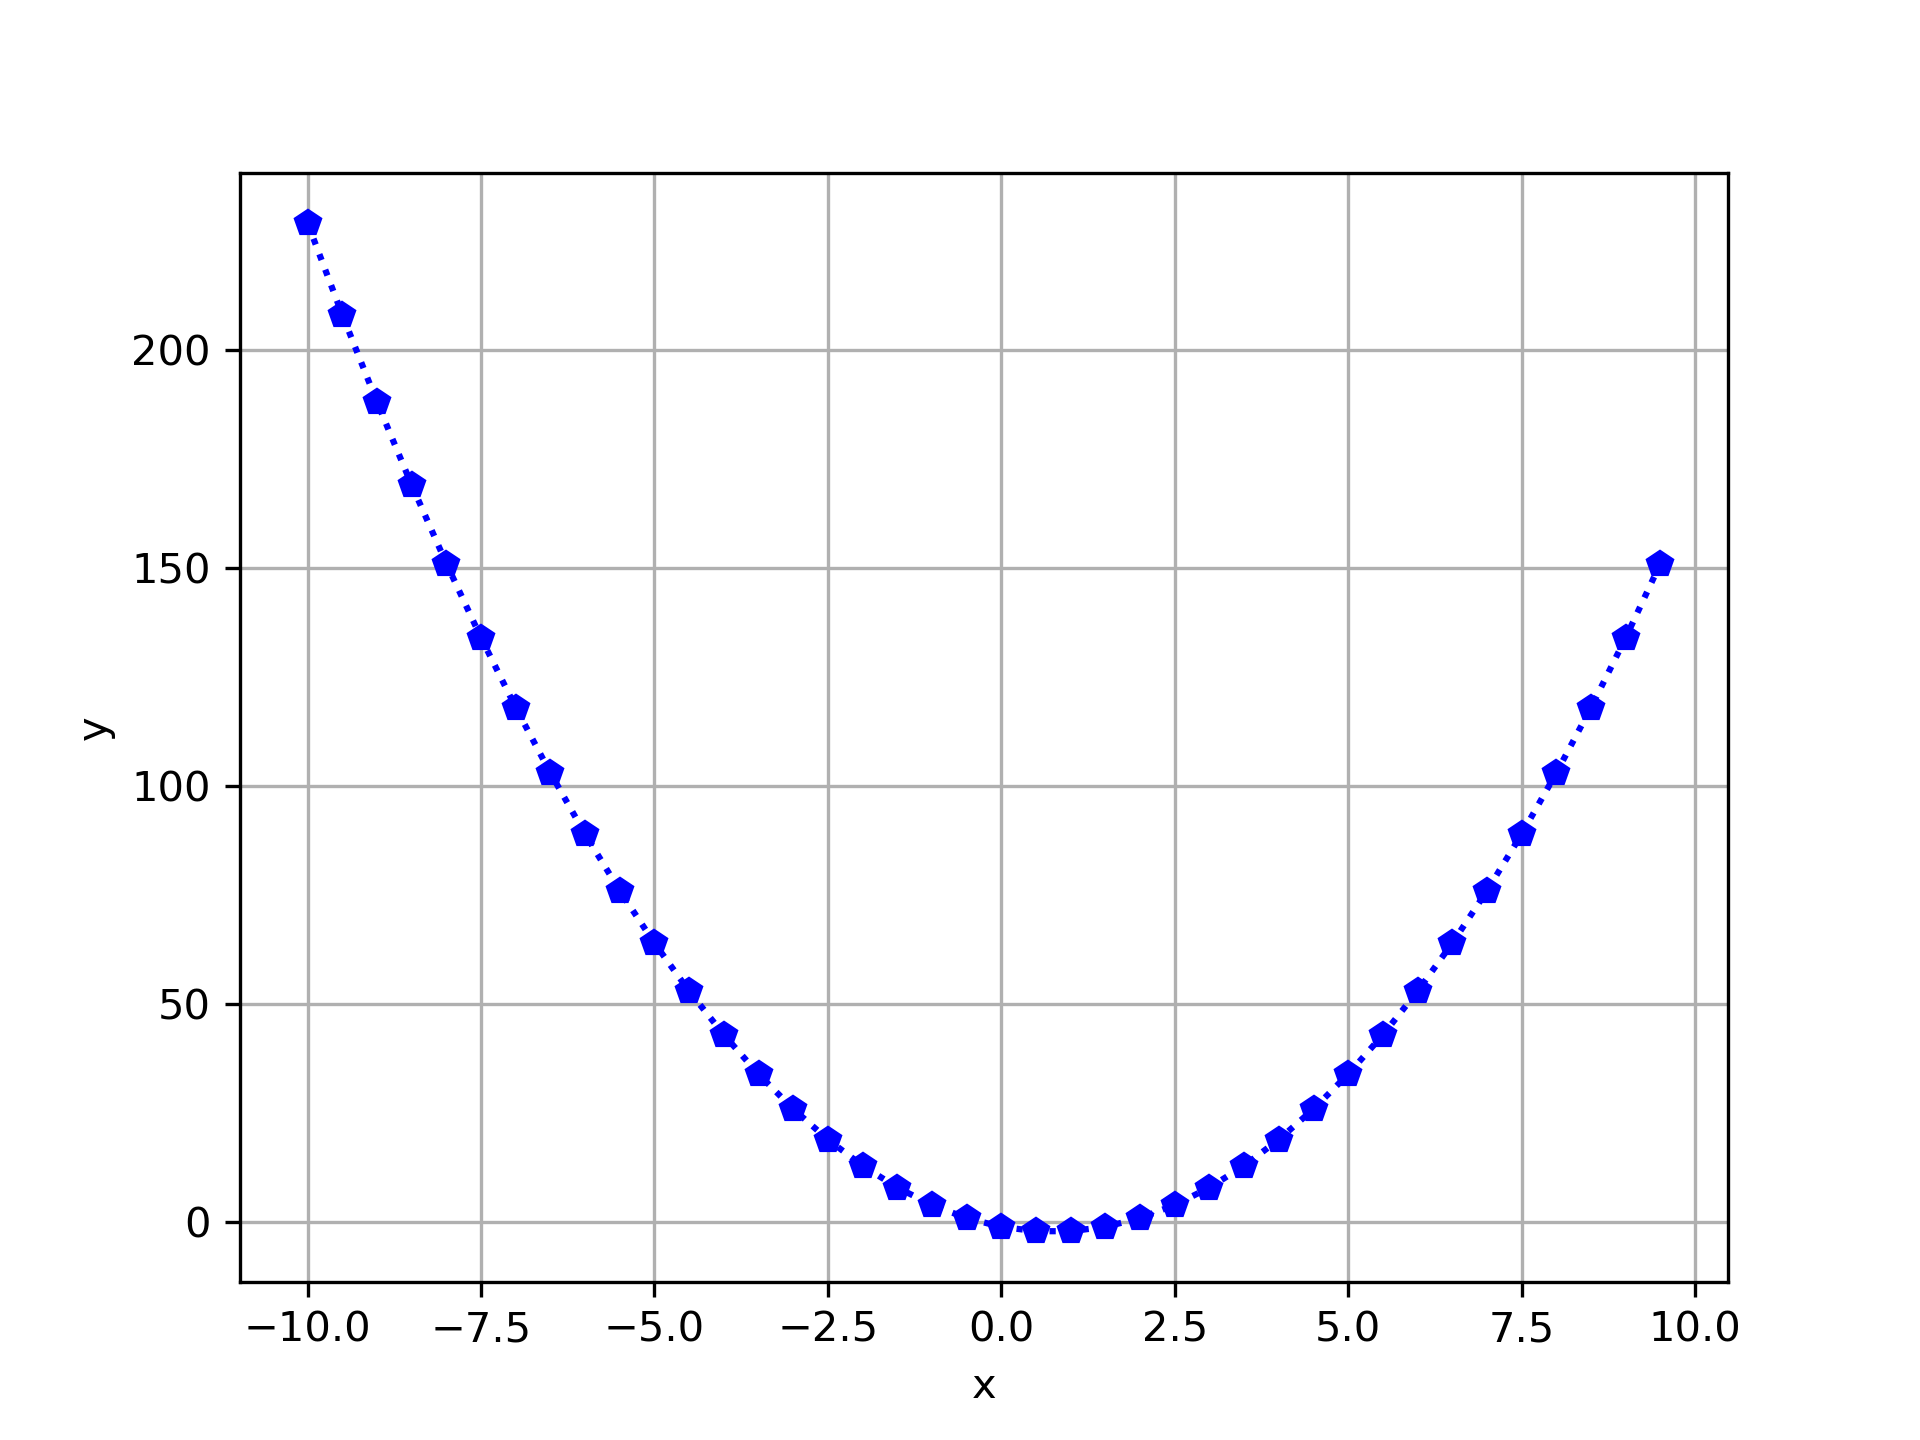
\includegraphics[width=400]{images/eqcurve.png}
\caption{\label{fig:SimpleSubplot}方程式曲線圖}
\end{figure}
\item \#2
\label{sec:orgbad5c35}
\begin{figure}[htbp]
\centering
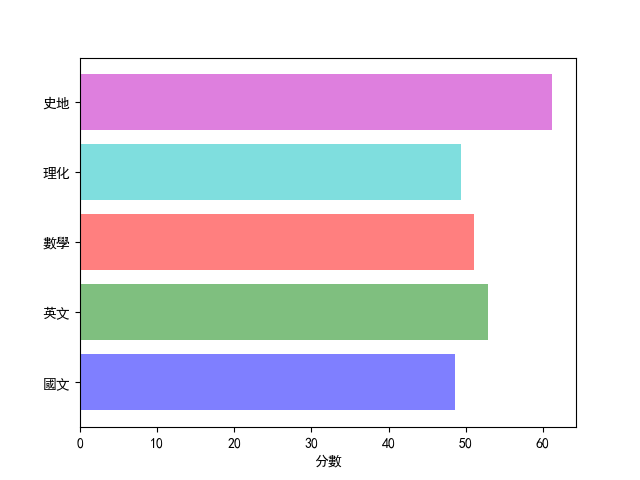
\includegraphics[width=400]{images/scobars.png}
\caption{\label{fig:SimpleSubplot}分數長條圖}
\end{figure}
\item \#3
\label{sec:org9064b82}
\begin{figure}[htbp]
\centering
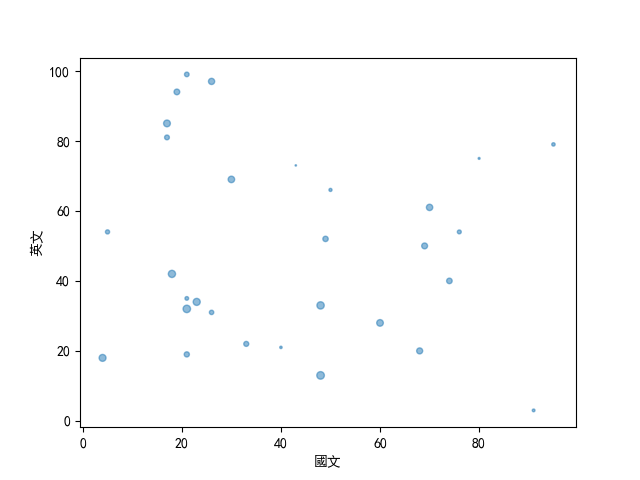
\includegraphics[width=400]{images/scosct.png}
\caption{\label{fig:SimpleSubplot}兩科成績的關係圖}
\end{figure}
\newpage
\end{enumerate}
\end{enumerate}

\section{Pandas}
\label{sec:orgc1437d0}
\subsection{Excel/CSV: Pandas 模組}
\label{sec:orge16f27f}
\begin{enumerate}
\item CSV
\label{sec:org71403ea}
\begin{itemize}
\item 為純文字檔，以逗號分隔值（Comma-Separated Values，CSV，有時也稱為字元分隔值，因為分隔字元也可以不是逗號）。\\
\item 純文字意味著該檔案是一個字元序列，不含必須像二進位制數字那樣被解讀的資料。\\
\item CSV 檔案由任意數目的記錄組成，記錄間以某種換行符分隔；每條記錄由欄位組成，欄位間的分隔符是其它字元或字串，最常見的是逗號。\\
\end{itemize}
\item Pandas
\label{sec:org6f709c0}
\begin{itemize}
\item Pandas 為建構於 NumPy 之上的套件，為 python 的一個數據分析模組，適合處理表格資料或\\
異質資料。\\
\item 於 2009 年底開源出來，提供高效能、簡易使用的\\
資料格式(Data Frame，為 R 語言主要資料格式)，可以讓使用者可以快速操作及分析資料。\\
\item Pandas 強化了資料處理的方便性也能與處理網頁資料與資料庫資料等，有點類似於\\
Office 的 Excel，能更加方便的進行運算、分析等\footnote{\href{https://blog.csdn.net/qq\_18668137/article/details/80807829}{conda、miniconda、anaconda的區別以及在pycharm中選擇conda的虛擬環境}\\}。\\
\item Pandas 主要特色有\textsuperscript{\ref{org43bd2be}}：\\
\begin{enumerate}
\item 在異質數據的讀取、轉換和處理上，都讓分析人員更容易處理，例如：從列欄試算表中找到想要的值。\\
\item Pandas 提供兩種主要的資料結構，Series 與 DataFrame。Series 顧名思義就是用來處理時間序列相關的資料(如感測器資料等)，主要為建立索引的一維陣列。DataFrame 則是用來處理結構化(Table like)的資料，有列索引與欄標籤的二維資料集，例如關聯式資料庫、CSV 等等。\\
\item 透過載入至 Pandas 的資料結構物件後，可以透過結構化物件所提供的方法，來快速地進行資料的前處理，如資料補值，空值去除或取代等。\\
\item 更多的輸入來源及輸出整合性，例如：可以從資料庫讀取資料進入 Dataframe，也可將處理完的資料存回資料庫。\\
\end{enumerate}
\end{itemize}
\end{enumerate}
\subsection{Pandas 資料結構}
\label{sec:org9fae0d3}
Pandas 兩類資料結構\textsuperscript{\ref{org9a526ba}}：\footnote{\href{https://oranwind.org/python-pandas-ji-chu-jiao-xue/}{[Python] Pandas 基礎教學}\\}\\
\begin{enumerate}
\item Series: 用來處理時間序列相關的資料(如感測器資料等)，主要為建立索引的一維陣列。\\
\item DataFrame: 是一個二維標籤資料結構，可以具有不同類型的行（column），類似 Excel\\
的資料表，對於有使用過統計軟體的分析人員應該不陌生。簡單來說，Series 可以想像\\
為一行多列（row）的資料，而 DataFrame 是多行多列的資料，藉由選擇索引（列標籤）\\
和行（行標籤）的參數來操作資料，就像使用統計軟體透過樣本編號或變項名稱來操作\\
資料。\\
\end{enumerate}
\subsection{Series}
\label{sec:orgf619e13}
\begin{enumerate}
\item 建立: 資料類型可為 array, dictionary
\label{sec:org538e382}
\begin{itemize}
\item 由 array 建立 Series\\
\end{itemize}
\lstset{breaklines=true,language=Python,label= ,caption= ,captionpos=b,firstnumber=1,numbers=left}
\begin{lstlisting}
import pandas as pd

cars = ["SAAB", "Audi", "BMW", "BENZ", "Toyota", "Nissan", "Lexus"]
print("資料型別:", type(cars))
carsToSeries = pd.Series(cars)
print("資料型別:", type(carsToSeries))
print(carsToSeries.shape)
print(carsToSeries)
print("carsToSeries[1]: ", carsToSeries[1])
\end{lstlisting}

\begin{verbatim}
資料型別: <class 'list'>
資料型別: <class 'pandas.core.series.Series'>
(7,)
0      SAAB
1      Audi
2       BMW
3      BENZ
4    Toyota
5    Nissan
6     Lexus
dtype: object
carsToSeries[1]:  Audi
\end{verbatim}

\item 資料篩選
\label{sec:org6fcb5a2}
\begin{itemize}
\item 選擇\\
\end{itemize}
\lstset{breaklines=true,language=Python,label= ,caption= ,captionpos=b,firstnumber=1,numbers=left}
\begin{lstlisting}
import pandas as pd

dict = {
    "city": "Kaohsiung",
    "speedCamera1": "13213",
    "speedCamera2": "3242",
    "speedCamera3": "134343",
    "speedCamera4": "4312",
    "speedCamera5": "533"
}

dictToSeries = pd.Series(dict, index = dict.keys()) # 排序與原 dict 相同
print(dictToSeries[0])
print("=====")
print(dictToSeries['speedCamera1'])
print("=====")
print(dictToSeries[[0, 2, 4]])
print("=====")
print(dictToSeries[['city', 'speedCamera1', 'speedCamera3']])
print("=====")
print(dictToSeries[:2])
print("=====")
print(dictToSeries[4:])
\end{lstlisting}

\begin{verbatim}
Kaohsiung
=====
13213
=====
city            Kaohsiung
speedCamera2         3242
speedCamera4         4312
dtype: object
=====
city            Kaohsiung
speedCamera1        13213
speedCamera3       134343
dtype: object
=====
city            Kaohsiung
speedCamera1        13213
dtype: object
=====
speedCamera4    4312
speedCamera5     533
dtype: object
\end{verbatim}
\end{enumerate}

\subsection{DataFrame}
\label{sec:org3114fb3}
\begin{enumerate}
\item DataFrame 建立
\label{sec:orgc0508f3}
可利用 Dictionary 或是 Array 來建立，並使用 DataFrame 的方法來操作資料查看、資料篩選、資料切片、資料排序等運算。\\
\item 由 Dictionary 建立
\label{sec:org5259300}
\lstset{breaklines=true,language=Python,label= ,caption= ,captionpos=b,firstnumber=1,numbers=left}
\begin{lstlisting}
import pandas as pd

hobby = ["Movies", "Sports", "Coding", "Fishing", "Dancing", "cooking"]
count = [46, 8, 12, 12, 6, 58]

dict = {"hobby": hobby,
        "count": count
       }
print(dict)
df = pd.DataFrame(dict)
print(df)
\end{lstlisting}

\begin{verbatim}
{'hobby': ['Movies', 'Sports', 'Coding', 'Fishing', 'Dancing', 'cooking'], 'count': [46, 8, 12, 12, 6, 58]}
     hobby  count
0   Movies     46
1   Sports      8
2   Coding     12
3  Fishing     12
4  Dancing      6
5  cooking     58
\end{verbatim}

\item 由 Array 建立
\label{sec:org3b45d68}
\lstset{breaklines=true,language=Python,label= ,caption= ,captionpos=b,firstnumber=1,numbers=left}
\begin{lstlisting}
import pandas as pd

ary = [["Movies", 46],["Sports", 8], ["Coding", 12], ["Fishing",12], ["Dancing",6], ["cooking",8]]
print(ary)
ary2df = pd.DataFrame(ary, columns = ["hobby", "count"]) # 指定欄標籤名稱
print(ary2df)

\end{lstlisting}

\begin{verbatim}
[['Movies', 46], ['Sports', 8], ['Coding', 12], ['Fishing', 12], ['Dancing', 6], ['cooking', 8]]
     hobby  count
0   Movies     46
1   Sports      8
2   Coding     12
3  Fishing     12
4  Dancing      6
5  cooking      8
\end{verbatim}

\item 讀入已存在的資料檔來建立 Dataframe
\label{sec:org85b06ec}
\begin{itemize}
\item 可以從異質資料來源讀取檔案(如 CSV 檔)內容，並將資料放入 DataFrame 中，進行資料查看、資料篩選、資料切片等運算。\\
\item 如果資料檔和程式放在同一目錄(資料夾)\\
\item 如果資料檔放在本機在其他地方\\
\begin{itemize}
\item 絕對路徑\\
\item 相對路徑\\
\end{itemize}
\item \href{./scores.csv}{下載範例檔:scores.csv}\\
\end{itemize}
\lstset{breaklines=true,language=Python,label= ,caption= ,captionpos=b,firstnumber=1,numbers=left}
\begin{lstlisting}
import pandas as pd

# 讀取csv
df = pd.read_csv("scores.csv")
print("===全部資料===")
print(df)


\end{lstlisting}

\begin{verbatim}
===全部資料===
            id  classparti  typing  homework  midexam  finalexam
0    201910901         100      72     92.11     48.0       16.0
1    201910902          96      56     93.42     60.0       40.0
2    201910903          96      76    102.63     45.0       28.0
3    201910904          93      64     86.84     44.0       25.0
4    201910905          93      56     42.11      0.0       20.0
..         ...         ...     ...       ...      ...        ...
207  201911726         106      80    102.63     96.5      103.0
208  201911727          82      60    102.63     84.0      100.0
209  201911728          83      48    102.63     83.0       75.0
210  201911729          87      84    105.26    112.3      103.0
211  201911730          96      72    102.63     91.0      100.0

[212 rows x 6 columns]
\end{verbatim}
\end{enumerate}

\subsection{DataFrame 的資料瀏覽}
\label{sec:orga27a563}
\begin{enumerate}
\item 碁本函數
\label{sec:orgd8bf365}
\begin{itemize}
\item shape\\
\item describe()\\
\item head()\\
\item tail()\\
\item columns\\
\item index\\
\item info()\\
\end{itemize}
\lstset{breaklines=true,language=Python,label= ,caption= ,captionpos=b,firstnumber=1,numbers=left}
\begin{lstlisting}
import pandas as pd

hobby = ["Movies", "Sports", "Coding", "Fishing", "Dancing", "cooking"]
count = [46, 8, 12, 12, 6, 58]

dict = {"hobby": hobby,
        "count": count
       }

df = pd.DataFrame(dict)
print(df)
print("====")
print(df.shape) # 回傳列數與欄數
print("---")
print(df.describe()) # 回傳描述性統計
print("---")
print(df.head(3)) # 回傳前三筆觀測值
print("---")
print(df.tail(3)) # 回傳後三筆觀測值
print("---")
print(df.columns) # 回傳欄位名稱
print("---")
print(df.index) # 回傳 index
print("---")
print(df.info) # 回傳資料內容
\end{lstlisting}

\begin{verbatim}
     hobby  count
0   Movies     46
1   Sports      8
2   Coding     12
3  Fishing     12
4  Dancing      6
5  cooking     58
====
(6, 2)
---
           count
count   6.000000
mean   23.666667
std    22.393451
min     6.000000
25%     9.000000
50%    12.000000
75%    37.500000
max    58.000000
---
    hobby  count
0  Movies     46
1  Sports      8
2  Coding     12
---
     hobby  count
3  Fishing     12
4  Dancing      6
5  cooking     58
---
Index(['hobby', 'count'], dtype='object')
---
RangeIndex(start=0, stop=6, step=1)
---
<bound method DataFrame.info of      hobby  count
0   Movies     46
1   Sports      8
2   Coding     12
3  Fishing     12
4  Dancing      6
5  cooking     58>
\end{verbatim}

\item DataFrame 資料排序
\label{sec:orgcfafc22}
\begin{itemize}
\item sort\_index(): The axis along which to sort. The value 0 identifies the rows, and 1 identifies the columns.\\
\item sort\_values()\\
\item sort 後的結果為複本，不改變原本的資料\\
\end{itemize}
\lstset{breaklines=true,language=Python,label= ,caption= ,captionpos=b,firstnumber=1,numbers=left}
\begin{lstlisting}
import pandas as pd

hobby = ["Movies", "Sports", "Coding", "Fishing", "Dancing", "cooking"]
count = [46, 8, 12, 12, 6, 58]

dict = {"hobby": hobby,
        "count": count
       }

df = pd.DataFrame(dict)
print("===Original")
print(df)
print("===.sort_index()")
print(df.sort_index(axis = 1, ascending = True))
print("===.sort_index()")
print(df.sort_index(axis = 0, ascending = False))
print("===.sort_values()")
print(df.sort_values(by = 'count'))
\end{lstlisting}

\begin{verbatim}
===Original
     hobby  count
0   Movies     46
1   Sports      8
2   Coding     12
3  Fishing     12
4  Dancing      6
5  cooking     58
===.sort_index()
   count    hobby
0     46   Movies
1      8   Sports
2     12   Coding
3     12  Fishing
4      6  Dancing
5     58  cooking
===.sort_index()
     hobby  count
5  cooking     58
4  Dancing      6
3  Fishing     12
2   Coding     12
1   Sports      8
0   Movies     46
===.sort_values()
     hobby  count
4  Dancing      6
1   Sports      8
2   Coding     12
3  Fishing     12
0   Movies     46
5  cooking     58
\end{verbatim}

\item DataFrame 處理遺漏值
\label{sec:org44b529c}
\begin{itemize}
\item dropna()\\
\item fillna()\\
\item isnull()\\
\item notnull()\\
\item 下載\url{scores-null.csv}\\
\end{itemize}
\lstset{breaklines=true,language=Python,label= ,caption= ,captionpos=b,firstnumber=1,numbers=left}
\begin{lstlisting}
import pandas as pd

df = pd.read_csv('scores-null.csv')
print(df)
# 刪除有遺失值的記錄
dropValue = df.dropna()
print(dropValue)
fill0 = df.fillna(0)
print(fill0)
fillv = df.fillna({"classparti":999, "typing":0, "finalExam":"NULL"})
print(fillv)
\end{lstlisting}

\begin{verbatim}
          id  classparti  typing  homework  finalExam
0  201910901       100.0    72.0     92.11       48.0
1  201910902        96.0    56.0     93.42       60.0
2  201910903        96.0    76.0    102.63        NaN
3  201910904         NaN    64.0     86.84       44.0
4  201910905        93.0    56.0     42.11        0.0
5  201910906       101.0   108.0    100.00        NaN
6  201910907       101.0     NaN     92.11       55.0
7  201910908        94.0    68.0    105.26       61.0
8  201910909         NaN    64.0     44.74       20.0
9  201910910        93.0   120.0     97.37       16.0
          id  classparti  typing  homework  finalExam
0  201910901       100.0    72.0     92.11       48.0
1  201910902        96.0    56.0     93.42       60.0
4  201910905        93.0    56.0     42.11        0.0
7  201910908        94.0    68.0    105.26       61.0
9  201910910        93.0   120.0     97.37       16.0
          id  classparti  typing  homework  finalExam
0  201910901       100.0    72.0     92.11       48.0
1  201910902        96.0    56.0     93.42       60.0
2  201910903        96.0    76.0    102.63        0.0
3  201910904         0.0    64.0     86.84       44.0
4  201910905        93.0    56.0     42.11        0.0
5  201910906       101.0   108.0    100.00        0.0
6  201910907       101.0     0.0     92.11       55.0
7  201910908        94.0    68.0    105.26       61.0
8  201910909         0.0    64.0     44.74       20.0
9  201910910        93.0   120.0     97.37       16.0
          id  classparti  typing  homework finalExam
0  201910901       100.0    72.0     92.11        48
1  201910902        96.0    56.0     93.42        60
2  201910903        96.0    76.0    102.63      NULL
3  201910904       999.0    64.0     86.84        44
4  201910905        93.0    56.0     42.11         0
5  201910906       101.0   108.0    100.00      NULL
6  201910907       101.0     0.0     92.11        55
7  201910908        94.0    68.0    105.26        61
8  201910909       999.0    64.0     44.74        20
9  201910910        93.0   120.0     97.37        16
\end{verbatim}
\end{enumerate}

\subsection{Dataframe 的選取與過濾}
\label{sec:orgc07000a}

\begin{enumerate}
\item 資料選取: Select column(s) \footnote{\href{https://www.itread01.com/content/1547569271.html}{Python讀寫csv檔案的幾種方法 及 pandas.read\textsubscript{csv} 引數全解}\\}
\label{sec:org6a098c9}
\begin{itemize}
\item \lstinline[breaklines=true,language=Python]~ df[['col1', 'col2']] ~\\
\item \lstinline[breaklines=true,language=Python]~ df.col1 ~\\
\end{itemize}
\lstset{breaklines=true,language=Python,label= ,caption= ,captionpos=b,firstnumber=1,numbers=left}
\begin{lstlisting}
import pandas as pd

df = pd.read_csv("scores.csv")
print(df.head(3))
print(df[['id', 'typing']].head(3))
print(df.id, df.homework)
\end{lstlisting}

\begin{verbatim}
          id  classparti  typing  homework  midexam  finalexam
0  201910901         100      72     92.11     48.0       16.0
1  201910902          96      56     93.42     60.0       40.0
2  201910903          96      76    102.63     45.0       28.0
          id  typing
0  201910901      72
1  201910902      56
2  201910903      76
0      201910901
1      201910902
2      201910903
3      201910904
4      201910905
         ...    
207    201911726
208    201911727
209    201911728
210    201911729
211    201911730
Name: id, Length: 212, dtype: int64 0       92.11
1       93.42
2      102.63
3       86.84
4       42.11
        ...  
207    102.63
208    102.63
209    102.63
210    105.26
211    102.63
Name: homework, Length: 212, dtype: float64
\end{verbatim}

\item 資料選取: Select using index (row)
\label{sec:org92a92e7}
\begin{itemize}
\item \lstinline[breaklines=true,language=Python]~ df[1:20] ~\\
\end{itemize}
\lstset{breaklines=true,language=Python,label= ,caption= ,captionpos=b,firstnumber=1,numbers=left}
\begin{lstlisting}
import pandas as pd

df = pd.read_csv("scores.csv")

print(df[1:3])
print(df[df.homework<30])
# 合併row and column
print(df.id[df.homework<30])
print(df[['id', 'homework']][1:3])
\end{lstlisting}

\begin{verbatim}
          id  classparti  typing  homework  midexam  finalexam
1  201910902          96      56     93.42     60.0       40.0
2  201910903          96      76    102.63     45.0       28.0
            id  classparti  typing  homework  midexam  finalexam
10   201910911          62      44     20.39      4.0        0.0
18   201910919          14      56     25.92      0.0        0.0
23   201910924          75      48     10.75      0.0        0.0
124  201911315          71     120     15.35      0.0        0.0
140  201911331          93     120     25.88      0.0       16.0
10     201910911
18     201910919
23     201910924
124    201911315
140    201911331
Name: id, dtype: int64
          id  homework
1  201910902     93.42
2  201910903    102.63
\end{verbatim}

\item 條件式選取資料
\label{sec:org15f64f6}
\begin{enumerate}
\item 語法
\label{sec:orgb3d1e61}
\begin{itemize}
\item \lstinline[breaklines=true,language=Python]~ df[(condition)] ~\\
\item \lstinline[breaklines=true,language=Python]~ df[(condition 1) & (condition 2) ] ~\\
\end{itemize}
\item 範例
\label{sec:org0954901}
\lstset{breaklines=true,language=Python,label= ,caption= ,captionpos=b,firstnumber=1,numbers=left}
\begin{lstlisting}
import pandas as pd

df = pd.read_csv("scores.csv")

print(df[(df.midexam >= 100) & (df.finalexam >= 100)])
\end{lstlisting}

\begin{verbatim}
            id  classparti  typing  homework  midexam  finalexam
11   201910912          87      92     92.11    110.8     103.75
70   201911034         104      92    102.63    100.8     101.00
88   201911115         120      88    105.26    113.5     111.00
98   201911125         119      80    107.89    113.2     115.00
102  201911129         106      52    102.63    103.6     100.00
127  201911318         108      80    102.63    104.8     100.00
138  201911329         105      48    107.89    100.0     100.00
143  201911334         100     120     81.58    104.8     113.00
153  201911608          88       0    102.63    100.0     100.00
169  201911624          82     100    102.63    101.5     105.00
182  201911701         103     108     92.63    100.0     100.00
189  201911708         106     108    102.63    107.2     101.00
190  201911709         108      88    107.89    104.8     105.00
191  201911710         102     100    102.63    100.0     105.00
193  201911712         105      96    101.58    107.5     100.00
195  201911714         102      44    107.89    110.0     110.00
196  201911715         106     120    107.89    102.4     105.00
198  201911717          80     120    107.89    106.0     100.00
201  201911721         109      76    100.00    100.0     100.00
203  201911722         105     120    102.63    101.5     105.00
210  201911729          87      84    105.26    112.3     103.00
\end{verbatim}
\end{enumerate}
\end{enumerate}

\subsection{Dataframe 進階條件過濾}
\label{sec:org1c7355e}
\begin{enumerate}
\item loc, iloc, between \footnote{\href{https://ithelp.ithome.com.tw/articles/10208412}{Day23- 資料處理模組-Pandas 介紹}\\}
\label{sec:org90181cf}
\begin{itemize}
\item loc: 基於行標籤和列標籤（x\_label、y\_label）進行索引，以 column 名做為 index\\
\item iloc: 基於行索引和列索引（index，columns） 都是從 0 開始，以數字做為 index\\
\item between: 檢查區間值, \lstinline[breaklines=true,language=Python]~ Series.between(self, left, right, inclusive=True) ~\\
\end{itemize}
\begin{enumerate}
\item 範例 1
\label{sec:orgffc23fc}
\lstset{breaklines=true,language=Python,label= ,caption= ,captionpos=b,firstnumber=1,numbers=left}
\begin{lstlisting}
import pandas as pd

df = pd.read_csv("scores.csv")
print(df.head(3))
print("========")
print(df.loc[df.homework<25, ['id', 'homework']])
print("========")
print(df.loc[2,'homework'])
\end{lstlisting}

\begin{verbatim}
          id  classparti  typing  homework  midexam  finalexam
0  201910901         100      72     92.11     48.0       16.0
1  201910902          96      56     93.42     60.0       40.0
2  201910903          96      76    102.63     45.0       28.0
========
            id  homework
10   201910911     20.39
23   201910924     10.75
124  201911315     15.35
========
102.63
\end{verbatim}
\item 範例 2
\label{sec:org587a567}
\lstset{breaklines=true,language=Python,label= ,caption= ,captionpos=b,firstnumber=1,numbers=left}
\begin{lstlisting}
# 載入函式庫
import pandas as pd

print("Pandas version:", pd.__version__)
# 讀取csv
df = pd.read_csv("scores.csv")
# 輸出前3筆
print(df.iloc[:3])
# 輸出前3筆的第2,3欄
print(df.iloc[:2, 1:3])

print(df['midexam'].between(50, 60))
midFilter = df['midexam'].between(50, 55)
print(df[midFilter])
\end{lstlisting}

\begin{verbatim}
Pandas version: 0.25.1
          id  classparti  typing  homework  midexam  finalexam
0  201910901         100      72     92.11     48.0       16.0
1  201910902          96      56     93.42     60.0       40.0
2  201910903          96      76    102.63     45.0       28.0
   classparti  typing
0         100      72
1          96      56
0      False
1       True
2      False
3      False
4      False
       ...  
207    False
208    False
209    False
210    False
211    False
Name: midexam, Length: 212, dtype: bool
            id  classparti  typing  homework  midexam  finalexam
6    201910907         101     120     92.11     55.0       20.0
65   201911029          93      60     82.00     50.0       16.0
72   201911036          88      80    102.63     53.0       76.0
92   201911119          82     104     89.47     50.0       20.0
94   201911121          95     100     88.51     52.0       72.0
109  201911136          91     100     81.58     51.0        4.0
171  201911626          98      72     97.37     50.0       75.0
\end{verbatim}
\end{enumerate}
\end{enumerate}

\subsection{進階分析}
\label{sec:orgc413478}
\begin{enumerate}
\item 由其他 column 產生新的 column
\label{sec:orgac86a66}
\begin{itemize}
\item 全部指定\\
\item 條件指定\\
\end{itemize}
\item 資料分組: groupby
\label{sec:org791c67a}
\item 範例
\label{sec:org9da7f07}
\lstset{breaklines=true,language=Python,label= ,caption= ,captionpos=b,firstnumber=1,numbers=left}
\begin{lstlisting}
# 載入函式庫
import pandas as pd

# 讀取csv
df = pd.read_csv("scores.csv")
print(df.head(3))
# 計算總分'
df['Final'] = df.classparti*.1 + df.typing*.1 + df.homework*.2 + df.midexam*.3 + df.finalexam*.3

# PASS/FAIL
df.loc[df.Final < 60, 'PASS'] = False
df.loc[df.Final >= 60, 'PASS'] = True

# create new column according to typing speed
df.loc[df.typing < 30, 'TypingSpeed' ] = 'LOW'
df.loc[df.typing.between(30, 60), 'TypingSpeed' ] = 'MID'
df.loc[df.typing > 60, 'TypingSpeed' ] = 'HIGH'

print(df.head(3))

# 依打字速度分組
print(df.groupby('TypingSpeed')['Final'].mean())
print(df.groupby('PASS')['typing' ,'homework'].mean())

\end{lstlisting}

\begin{verbatim}
          id  classparti  typing  homework  midexam  finalexam
0  201910901         100      72     92.11     48.0       16.0
1  201910902          96      56     93.42     60.0       40.0
2  201910903          96      76    102.63     45.0       28.0
          id  classparti  typing  ...   Final   PASS  TypingSpeed
0  201910901         100      72  ...  54.822  False         HIGH
1  201910902          96      56  ...  63.884   True          MID
2  201910903          96      76  ...  59.626  False         HIGH

[3 rows x 9 columns]
TypingSpeed
HIGH    69.977451
LOW     68.517333
MID     64.086303
Name: Final, dtype: float64
          typing   homework
PASS                       
False  77.567568  76.409054
True   84.525547  96.350730
\end{verbatim}

\item 資料檔下載: \url{scores.csv}
\label{sec:org6bee7f7}
\end{enumerate}

\subsection{資料視覺化}
\label{sec:orge32503b}
\begin{enumerate}
\item Bar chart
\label{sec:org657d102}
\lstset{breaklines=true,language=Python,label= ,caption= ,captionpos=b,firstnumber=1,numbers=left}
\begin{lstlisting}
# 載入函式庫
import pandas as pd

# 讀取csv
df = pd.read_csv("scores.csv")

# 計算總分'
df['Final'] = df.classparti*.1 + df.typing*.1 + df.homework*.2 + df.midexam*.3 + df.finalexam*.3

# create new column according to typing speed
df.loc[df.typing < 30, 'TypingSpeed' ] = 'Level-1'
df.loc[df.typing.between(30, 60), 'TypingSpeed' ] = 'Level-2'
df.loc[df.typing > 60, 'TypingSpeed' ] = 'Level-3'

x = df.groupby('TypingSpeed')['homework','classparti'].mean()
print(x)

fig = df.groupby('TypingSpeed')['homework','classparti'].mean().plot(kind='bar', title="XXX", rot=0, legend=True)
fig.set_xlabel("Typing Speed")
fig.set_ylabel("score")
savefig = fig.get\under{}figure()
savefig.savefig('images/pandasPlot1.png', bbox_inches='tight')
\end{lstlisting}

\begin{figure}[htbp]
\centering
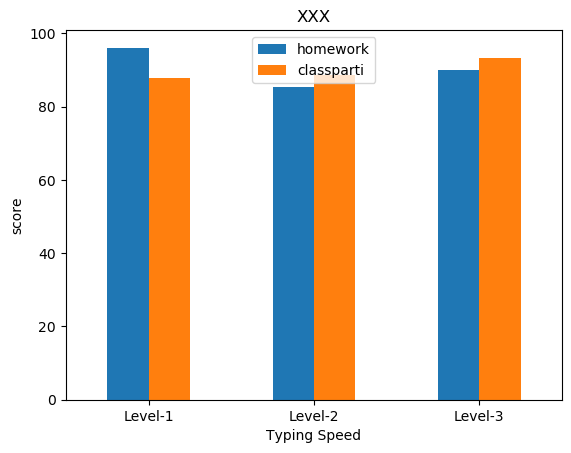
\includegraphics[width=300]{images/pandasPlot1.png}
\caption{\label{fig:PandasPlot-1}Pandas plot bar chart}
\end{figure}

\item Pie chart
\label{sec:org0a8b698}
\begin{enumerate}
\item DEMO
\label{sec:org4a762b0}
\lstset{breaklines=true,language=Python,label= ,caption= ,captionpos=b,firstnumber=1,numbers=left}
\begin{lstlisting}
# 載入函式庫
import pandas as pd

# 讀取csv
df = pd.read_csv("scores.csv")

# 計算總分'
df['Final'] = df.classparti*.1 + df.typing*.1 + df.homework*.2 + df.midexam*.3 + df.finalexam*.3

# create new column according to typing speed
df.loc[df.typing < 60, 'TypingSpeed' ] = 'Level-1'
df.loc[df.typing.between(60, 80), 'TypingSpeed' ] = 'Level-2'
df.loc[df.typing > 80, 'TypingSpeed' ] = 'Level-3'
print(df.groupby('TypingSpeed').count())

fig = df.groupby('TypingSpeed')['TypingSpeed'].count().plot(kind='pie', title="XXX", rot=0, legend=True)
savefig = fig.get\under{}figure()
savefig.savefig('images/pandasPlot2.png', bbox_inches='tight')
\end{lstlisting}

\begin{results}
\end{results}
\begin{results}
              id  classparti  typing  homework  midexam  finalexam  Final\\
TypingSpeed\\
Level-1       25          25      25        25       25         25     25\\
Level-2       86          86      86        86       86         86     86\\
Level-3      101         101     101       101      100        101    100\\
\end{results}

\begin{figure}[htbp]
\centering
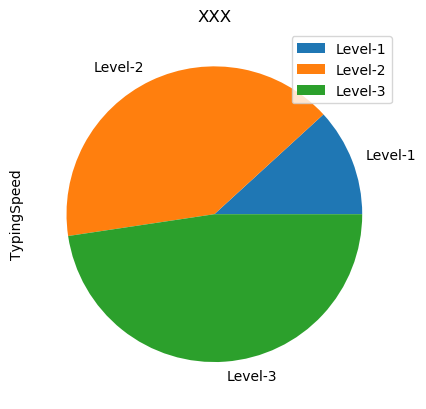
\includegraphics[width=400]{images/pandasPlot2.png}
\caption{\label{fig:PandasPlot-2}Pandas plot pie chart}
\end{figure}

\item 如何避免圖例擋住圖表
\label{sec:orgf16f7f2}
\begin{itemize}
\item \href{https://stackoverflow.com/questions/4700614/how-to-put-the-legend-out-of-the-plot}{How to put the legend out of the plot}\\
\end{itemize}
\end{enumerate}

\item Scatter chart
\label{sec:orge594852}
\lstset{breaklines=true,language=Python,label= ,caption= ,captionpos=b,firstnumber=1,numbers=left}
\begin{lstlisting}
# 載入函式庫
import pandas as pd

# 讀取csv
df = pd.read_csv("scores.csv")
  fig = df[['midexam','finalexam']].plot(kind='scatter', x=1, y=0)

  savefig = fig.get\under{}figure()
savefig.savefig('images/PandasPlot3.png')
\end{lstlisting}

\begin{figure}[htbp]
\centering
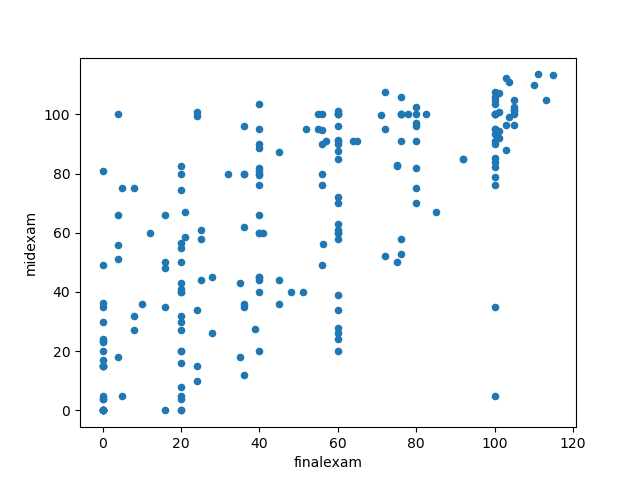
\includegraphics[width=400]{images/PandasPlot3.png}
\caption{\label{fig:PandasPlot-3}Pandas plot scatter chart}
\end{figure}

\item Haxbin chart
\label{sec:orgebc5330}
\lstset{breaklines=true,language=Python,label= ,caption= ,captionpos=b,firstnumber=1,numbers=left}
\begin{lstlisting}
# 載入函式庫
import pandas as pd

# 讀取csv
df = pd.read_csv("scores.csv")
fig = df[['midexam','finalexam']].plot(kind='hexbin', x=1, y=0, gridsize=25)

savefig = fig.get\under{}figure()
savefig.savefig('images/PandasPlot6.png')
\end{lstlisting}

\begin{figure}[htbp]
\centering
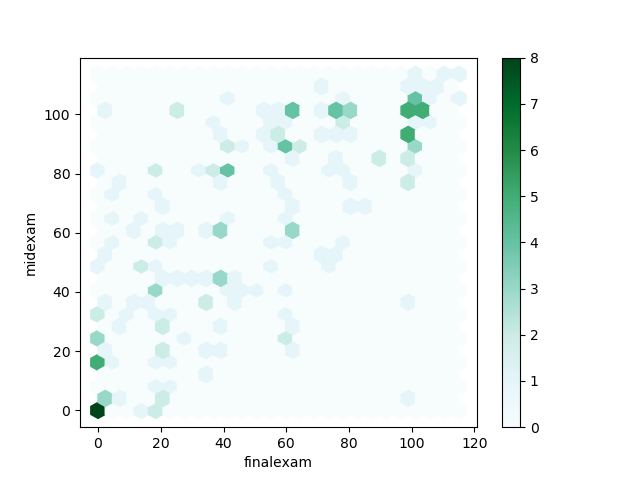
\includegraphics[width=400]{images/PandasPlot6.png}
\caption{\label{fig:PandasPlot-3}Pandas plot hexbin chart}
\end{figure}


\item Regression line chart
\label{sec:orgd725ff0}
\lstset{breaklines=true,language=Python,label= ,caption= ,captionpos=b,firstnumber=1,numbers=left}
\begin{lstlisting}
# 載入函式庫
import pandas as pd
import seaborn as sns

# 讀取csv
df = pd.read_csv("scores.csv")

fig = sns.regplot(x="midexam", y='finalexam', data=df);

savefig = fig.get\under{}figure()
savefig.savefig('images/PandasPlot4.png')

\end{lstlisting}

\begin{figure}[htbp]
\centering
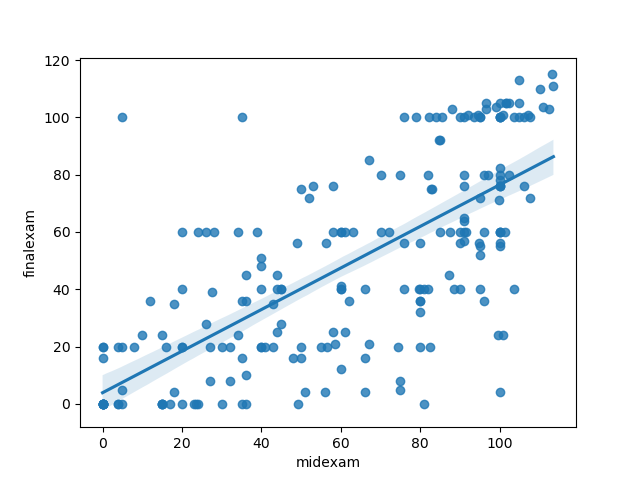
\includegraphics[width=400]{images/PandasPlot4.png}
\caption{\label{fig:PandasPlot-4}Pandas plot scatter chart}
\end{figure}
\end{enumerate}

\subsection{實作練習}
\label{sec:orgb654d5f}
\begin{enumerate}
\item 403 期中考得分統計
\label{sec:orgb596ec8}
\begin{itemize}
\item 原始數據\\
\end{itemize}
\begin{figure}[htbp]
\centering
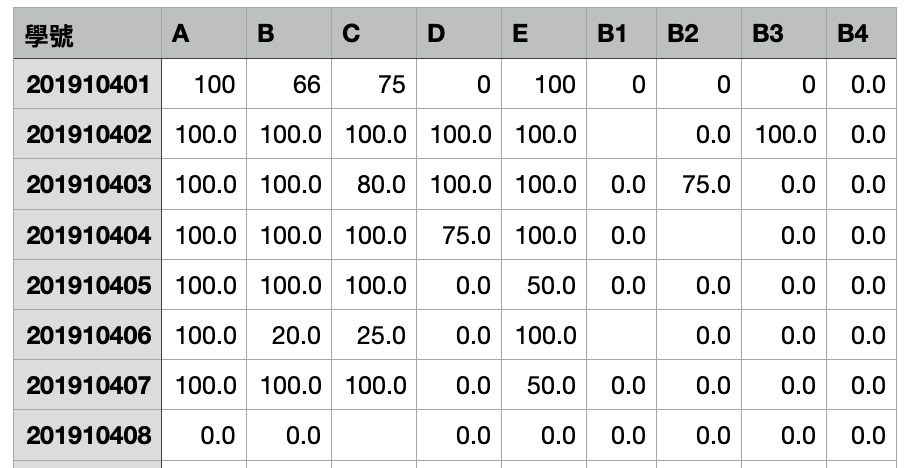
\includegraphics[width=400]{images/csv.jpg}
\caption{\label{fig:scoreCSV}CSV 內容}
\end{figure}
\begin{itemize}
\item \href{cs109score.csv}{cs109score.csv}為 T 市某校的資訊科線上期中考系統所匯出的成績檔，該次考試共計 10 題，\\
其中 A\textasciitilde{}F 為基本題，B1\textasciitilde{}B4 為加分題，前 5 題(A,B,C,D,E)為基本題，每題 100 分，後 4 題\\
為加分題(Bonus1\textasciitilde{}Bonus4)，每題 25 分，本份考卷總分：600；總得分除以 5 即為期中考得分，此次期中考總分 120 分。\\
\item 任務 1: 將有缺失值的部份以 0 分取代。\\
\item 任務 2: 求出每個人的原始總分(即所有分數)。\\
\item 任務 3: 求出換算得分(即總得分除以 5)。\\
\item 任務 4: 由學號欄提出班級資料， 新增一欄班級欄，班級為學號的第 5\textasciitilde{}7 碼，如 201910107，\\
表示該生為 101 班。\\
\item 任務 5: 求出各題的平均得分，以直條長條圖顯示。\\
\item 任務 6: 以班級為分組依據，畫出各班平均得分，以橫向長條圖顯示。\\
\item 任務 7: 求 119 班各題平均得分，以 pie chart 顯示。\\
\item 任務 8: 求所有受試者第 B 及 B1 兩題的 scatter plot 以及 regression line。\\
\end{itemize}
\lstset{breaklines=true,language=Python,label= ,caption= ,captionpos=b,firstnumber=1,numbers=left}
\begin{lstlisting}
}import numpy as np
import pandas as pd
import seaborn as sns
import matplotlib.pyplot as plt

origdf = pd.read_csv("cs109score.csv")

plt.rcParams['font.sans-serif'] = ['SimHei'] # 步驟一（替換sans-serif字型）
plt.rcParams['axes.unicode_minus'] = False  # 步驟二（解決座標軸負數的負號顯示問題）


##1
#origdf.fillna(0, inplace=True)
origdf = origdf.fillna(0)
##2
items = ['A', 'B', 'C', 'D', 'E', 'B1', 'B2' ,'B3', 'B4']
origdf['原始總分'] = origdf['A']+origdf['B']+origdf['C']+origdf['D']+origdf['E']+origdf['B1']+origdf['B2']+origdf['B3']+origdf['B4']
##3
origdf['分數'] = origdf['原始總分']/5
##4
origdf['班級'] = origdf['學號'].astype(str).str[4:7]
##5
y_pos = np.arange(len(items))
plt.bar(y_pos, origdf[items].mean(), color = ['b','g','r','c','m','y'], alpha=0.5)
plt.xticks(y_pos, items)
plt.xlabel('試題')
plt.savefig('images/task5.png')
plt.clf()
##6
fig = origdf.groupby('班級')['分數'].mean().plot(kind='barh', color = ['b','g','r','c','m','y'], alpha=0.5)
fig.set_xlabel('score')
fig.set_ylabel('班級', rotation=0)
resfig = fig.get\under{figure()
resfig.savefig('images/task6.png', bbox_inches='tight')
##7
df119 = origdf[(origdf.班級 == '119')]
plt.clf()
#print(df119[items].mean())
plt.pie(df119[items].mean(), labels = items)
plt.savefig('images/task7.png', dpi=300)
##8
import seaborn as sns
plt.clf()
fig = sns.regplot(x="A",  y="B", data=origdf)
                       resfig = fig.get\under{}figure()
resfig.savefig("images/task8.png")
\end{lstlisting}

\begin{figure}[htbp]
\centering
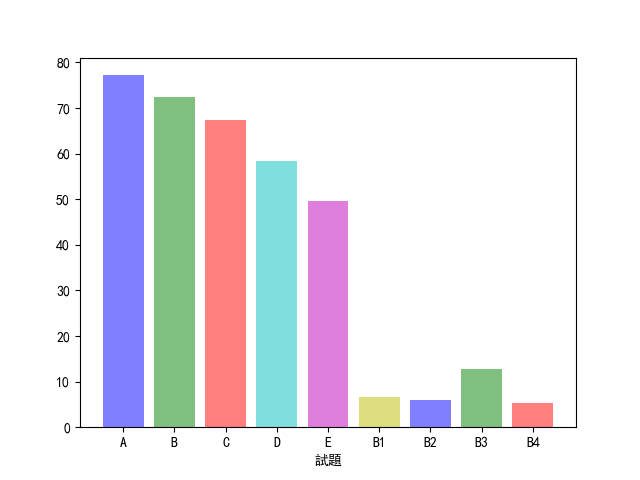
\includegraphics[width=400]{images/task5.png}
\caption{\label{fig:task5}task5}
\end{figure}
\begin{figure}[htbp]
\centering
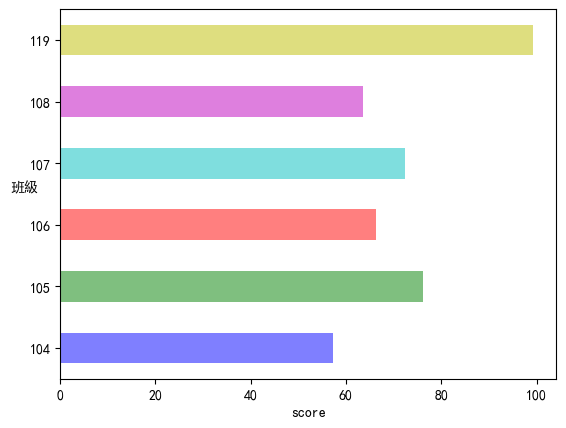
\includegraphics[width=400]{images/task6.png}
\caption{\label{fig:task6}task6}
\end{figure}
\begin{figure}[htbp]
\centering
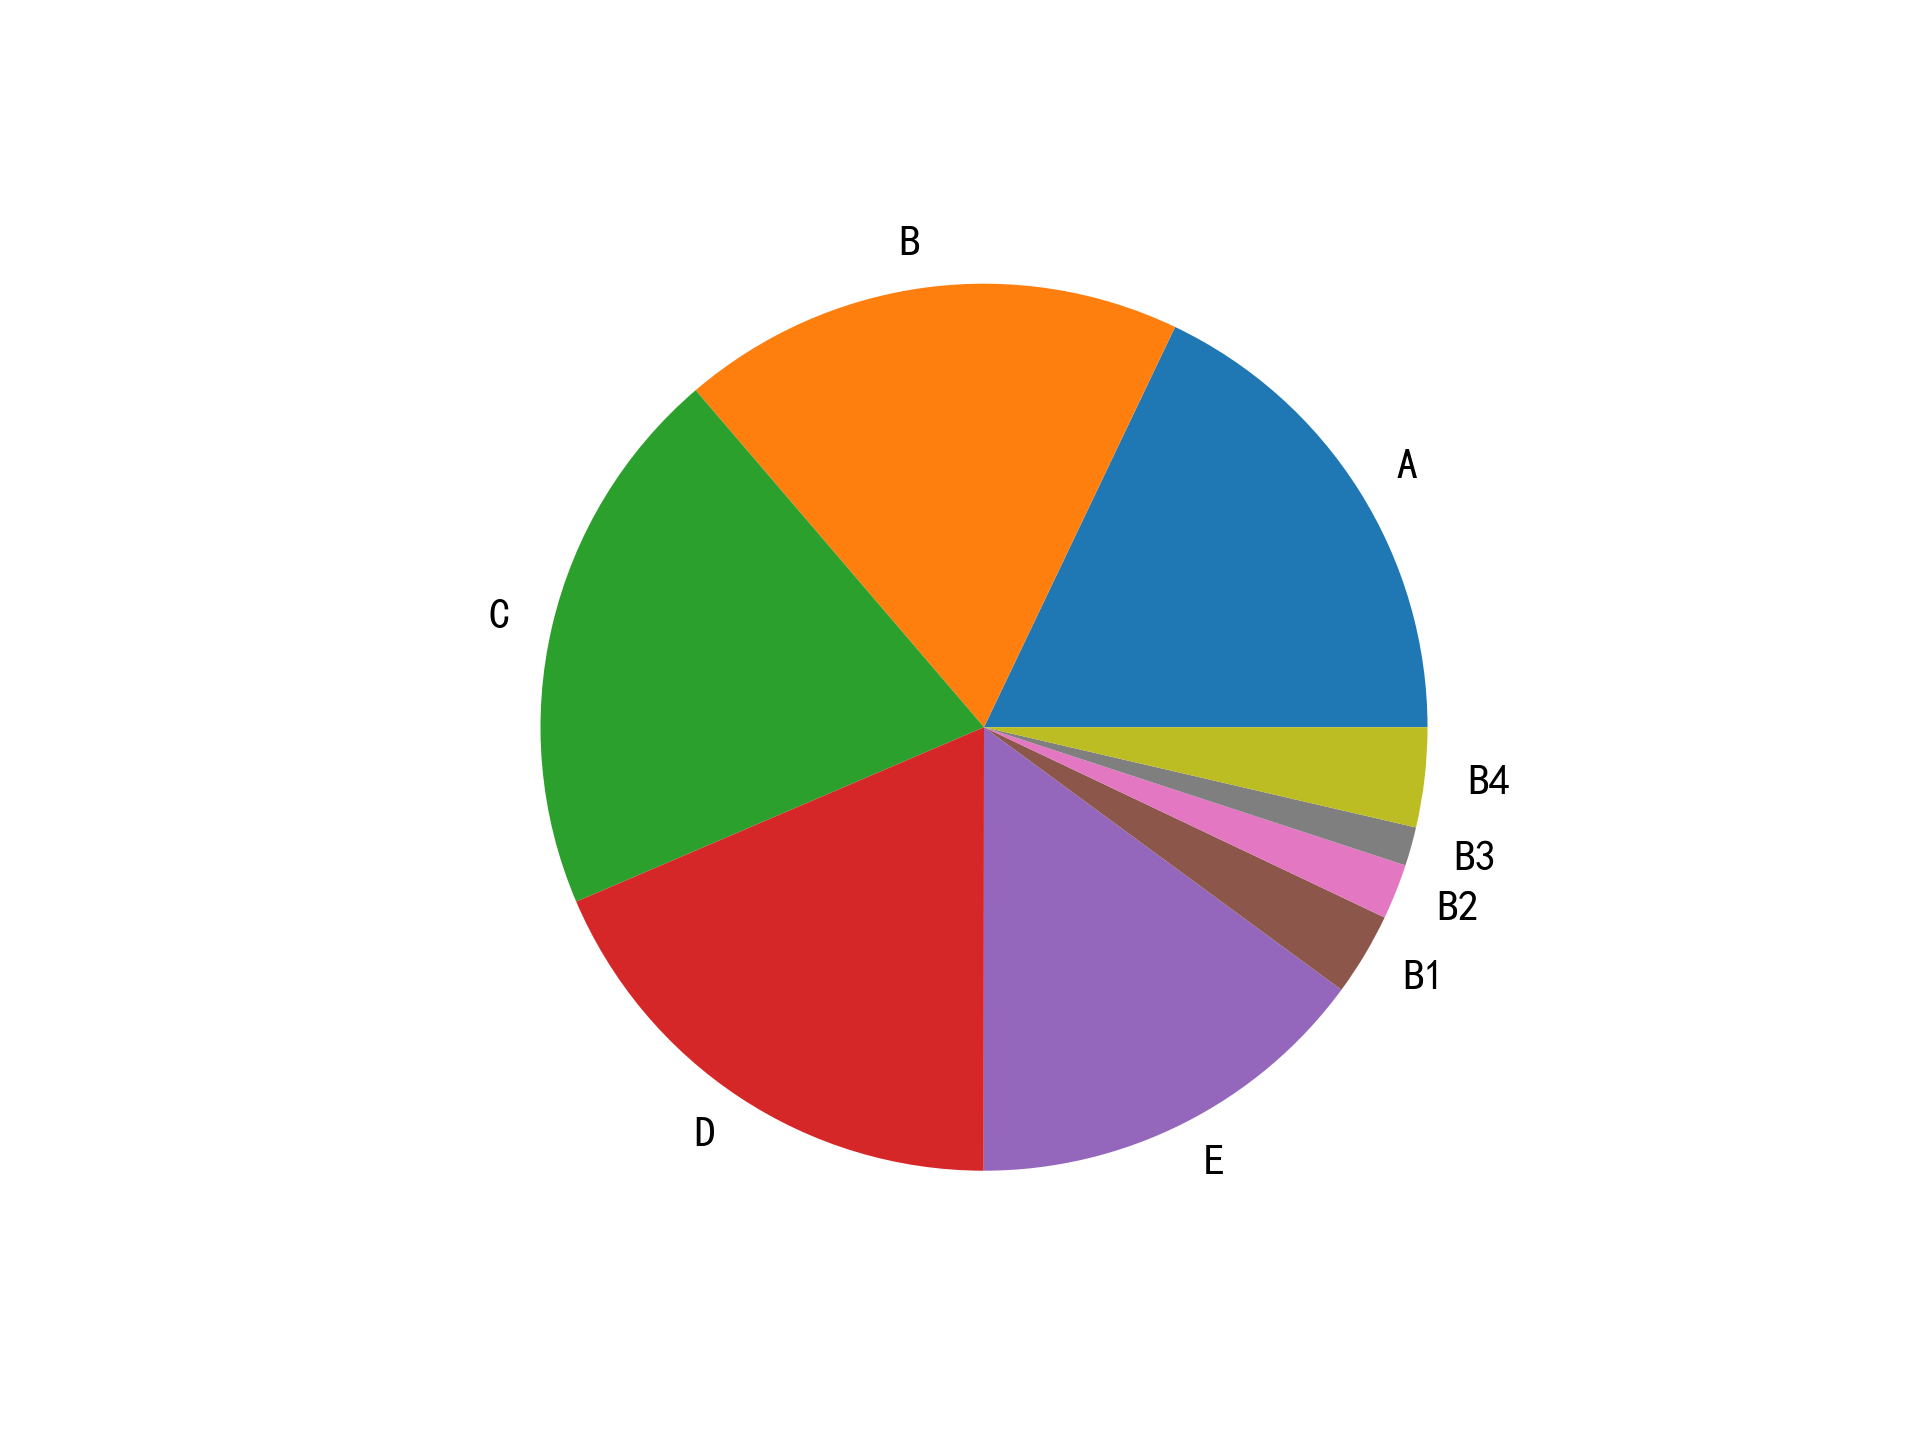
\includegraphics[width=400]{images/task7.png}
\caption{\label{fig:task7}task7}
\end{figure}
\begin{figure}[htbp]
\centering
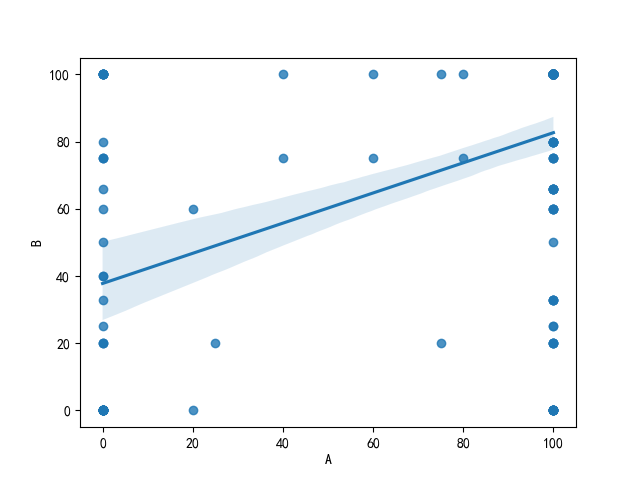
\includegraphics[width=400]{images/task8.png}
\caption{\label{fig:task}task8}
\end{figure}

\newpage
\end{enumerate}

\section{網路資料解析與爬蟲}
\label{sec:org728282f}
\subsection{網路資料分析的兩種類型}
\label{sec:orgaa94099}
\begin{itemize}
\item 可直接下載的靜態結構化資料，如 CSV、JSON、XML\\
\item 直接分析網站的線上內容(HTML): 爬蟲(Web Crawler)\\
\end{itemize}

\subsection{JSON}
\label{sec:orgef8efff}
\begin{enumerate}
\item What is JSON?
\label{sec:org7cb6ff7}
\begin{itemize}
\item JSON(JavaScript Object Notation，JavaScript 物件表示法)是個以純文字來描述\\
資料的簡單結構，在 JSON 中可以透過特定的格式去儲存任何資料(字串,數字,陣列,物件)，\\
也可以透過物件或陣列來傳送較複雜的資料。\footnote{\href{https://blog.wu-boy.com/2011/04/\%E4\%BD\%A0\%E4\%B8\%8D\%E5\%8F\%AF\%E4\%B8\%8D\%E7\%9F\%A5\%E7\%9A\%84-json-\%E5\%9F\%BA\%E6\%9C\%AC\%E4\%BB\%8B\%E7\%B4\%B9/}{你不可不知的 JSON 基本介紹}\\}\\
\item JSON 常用於網站上的資料呈現、傳輸 (例如將資料從伺服器送至用戶端，以利顯示網頁)。\\
\item 一旦建立了 JSON 資料，就可以非常簡單的跟其他程式溝通或交換資料，因為 JSON 就只\\
是純文字格式。\\
\end{itemize}
\item JSON 的優點
\label{sec:org68b7d05}
\begin{itemize}
\item 相容性高\\
\item 格式容易瞭解，閱讀及修改方便\\
\item 支援許多資料格式 (number,string,booleans,nulls,array,associative array)\\
\item 許多程式都支援函式庫讀取或修改 JSON 資料\\
\item NoSQL Database\\
\end{itemize}
\item JSON 結構
\label{sec:org02697f5}
\begin{itemize}
\item 物件: \{\}\\
\item 陣列: []\\
\end{itemize}
\item JSON 支援的資料格式
\label{sec:org0850568}
\begin{itemize}
\item 字串 (string)，要以雙引號括起來:\\
\begin{itemize}
\item \{``name'': ``Mike''\}\\
\end{itemize}
\item 數值 (number)\\
\begin{itemize}
\item \{``age'': 25\}\\
\end{itemize}
\item 布林值 (boolean)\\
\begin{itemize}
\item \{``pass'': True\}\\
\end{itemize}
\item 空值 (null)\\
\begin{itemize}
\item \{``middlename'': null\}\\
\end{itemize}
\item 物件 (object)\\
\item 陣列 (array)\\
\end{itemize}
\item JSON 物件
\label{sec:orgee92ec9}
\begin{itemize}
\item 格式\\
\item key 只能是字串，也一定要加上雙引號\\
\end{itemize}
\lstset{breaklines=true,language=Python,label= ,caption= ,captionpos=b,firstnumber=1,numbers=left}
\begin{lstlisting}
{
    "key1": value1,
    "key2": value2,
    ......
    "keyN": valueN
}
\end{lstlisting}

\begin{itemize}
\item 範例 1\\
\end{itemize}
\lstset{breaklines=true,language=Python,label= ,caption= ,captionpos=b,firstnumber=1,numbers=left}
\begin{lstlisting}
{
    "id": 1,
    "name": "Jamees, Yen",
    "price": 19,
    "gender": "M",
    "hobby": ["music", "programming"]
}
\end{lstlisting}

\begin{itemize}
\item 範例 2\\
\end{itemize}
\lstset{breaklines=true,language=Python,label= ,caption= ,captionpos=b,firstnumber=1,numbers=left}
\begin{lstlisting}
{
    "id": 382192
    "name": "Jamees, Yen",
    "price": 19,
    "gender": "M",
    "exams": [
        { "title": "期中考",
          "chinese": 85,
          "math": 98,
          "englihs": 92
        },
        { "title": "期末考",
          "chinese": 81,
          "math": 92,
          "englihs": 97
        }
    ],
    "hobby": ["music", "programming"]
}
\end{lstlisting}

\item 實作 1: \href{https://data.gov.tw/dataset/31897}{國際主要國家貨幣每月匯率概況}
\label{sec:orgdd16fed}
\begin{enumerate}
\item 下載 JSON
\label{sec:orgdae87b7}
\lstset{breaklines=true,language=Python,label= ,caption= ,captionpos=b,firstnumber=1,numbers=left}
\begin{lstlisting}
import requests

json_url = 'https://quality.data.gov.tw/dq_download_json.php?nid=11339&md5_url=f2fdbc21603c55b11aead08c84184b8f'
response = requests.get(json_url)

jsonRes = response.json()
print(type(jsonRes))
print(jsonRes[:3])
print('日期', ":", '美元／新台幣')
for item in jsonRes:
    print(item['日期'], ":", item['美元／新台幣'])
\end{lstlisting}

\begin{verbatim}
 1  <class 'list'>
 2  [
 3  {'日期': '2020/2/3',
 4    '美元／新台幣': '30.332',
 5    '人民幣／新台幣': '4.321461',
 6    '歐元／美元': '1.1077',
 7    '美元／日幣': '108.535',
 8    '英鎊／美元': '1.3147',
 9    '澳幣／美元': '0.6695',
10    '美元／港幣': '7.7685',
11    '美元／人民幣': '7.0189',
12    '美元／南非幣': '14.9376',
13    '紐幣／美元': '0.64675'},
14  {'日期': '2020/2/4',
15    '美元／新台幣': '30.207',
16    '人民幣／新台幣': '4.320537',
17    '歐元／美元': '1.1056',
18    '美元／日幣': '108.945',
19    '英鎊／美元': '1.29605',
20    '澳幣／美元': '0.67185',
21    '美元／港幣': '7.76895',
22    '美元／人民幣': '6.9915',
23    '美元／南非幣': '14.8117',
24    '紐幣／美元': '0.6466'},
25  {'日期': '2020/2/5',
26   '美元／新台幣': '30.152',
27   '人民幣／新台幣': '4.306248',
28   '歐元／美元': '1.1044',
29   '美元／日幣': '109.345',
30   '英鎊／美元': '1.3046',
31   '澳幣／美元': '0.6741',
32   '美元／港幣': '7.7644',
33   '美元／人民幣': '7.0019',
34   '美元／南非幣': '14.8205',
35   '紐幣／美元': '0.6484'}
36  ]
37  ==============================
38  日期 : 美元／新台幣
39  2020/2/3 : 30.332
40  2020/2/4 : 30.207
41  2020/2/5 : 30.152
42  2020/2/6 : 30.082
43  2020/2/7 : 30.126
44  2020/2/10 : 30.102
45  2020/2/11 : 30.068
46  2020/2/12 : 30.032
47  2020/2/13 : 30.037
48  2020/2/14 : 30.051
49  2020/2/17 : 30.056
50  2020/2/18 : 30.125
51  2020/2/19 : 30.152
52  2020/2/20 : 30.254
53  2020/2/21 : 30.403
54  2020/2/24 : 30.472
55  2020/2/25 : 30.402
56  2020/2/26 : 30.383
57  2020/2/27 : 30.33
58  2020/3/2 : 30.124
59  2020/3/3 : 30.087
60  2020/3/4 : 30.038
61  2020/3/5 : 29.96
62  2020/3/6 : 30.04
63  2020/3/9 : 30.13
64  2020/3/10 : 30.036
65  2020/3/11 : 30.095
66  2020/3/12 : 30.15
67  2020/3/13 : 30.21
68  2020/3/16 : 30.22
69  2020/3/17 : 30.25
70  2020/3/18 : 30.276
71  2020/3/19 : 30.506
72  2020/3/20 : 30.302
73  2020/3/23 : 30.405
74  2020/3/24 : 30.316
75  2020/3/25 : 30.325
76  2020/3/26 : 30.306
\end{verbatim}

\item 資料視覺化
\label{sec:orge93c069}
\lstset{breaklines=true,language=Python,label= ,caption= ,captionpos=b,firstnumber=1,numbers=left}
\begin{lstlisting}
import requests

json_url = 'https://quality.data.gov.tw/dq_download_json.php?nid=11339&md5_url=f2fdbc21603c55b11aead08c84184b8f'
response = requests.get(json_url)
jsonRes = response.json()

dates = [i['日期'] for i in jsonRes]
NTUS = [float(i['美元／新台幣']) for i in jsonRes]

import matplotlib.pyplot as plt

plt.clf()
plt.plot(dates, NTUS)
plt.xticks(rotation=60, fontsize=6)
plt.savefig('images/jsonLine.png', dpi=300)
\end{lstlisting}

\begin{figure}[htbp]
\centering
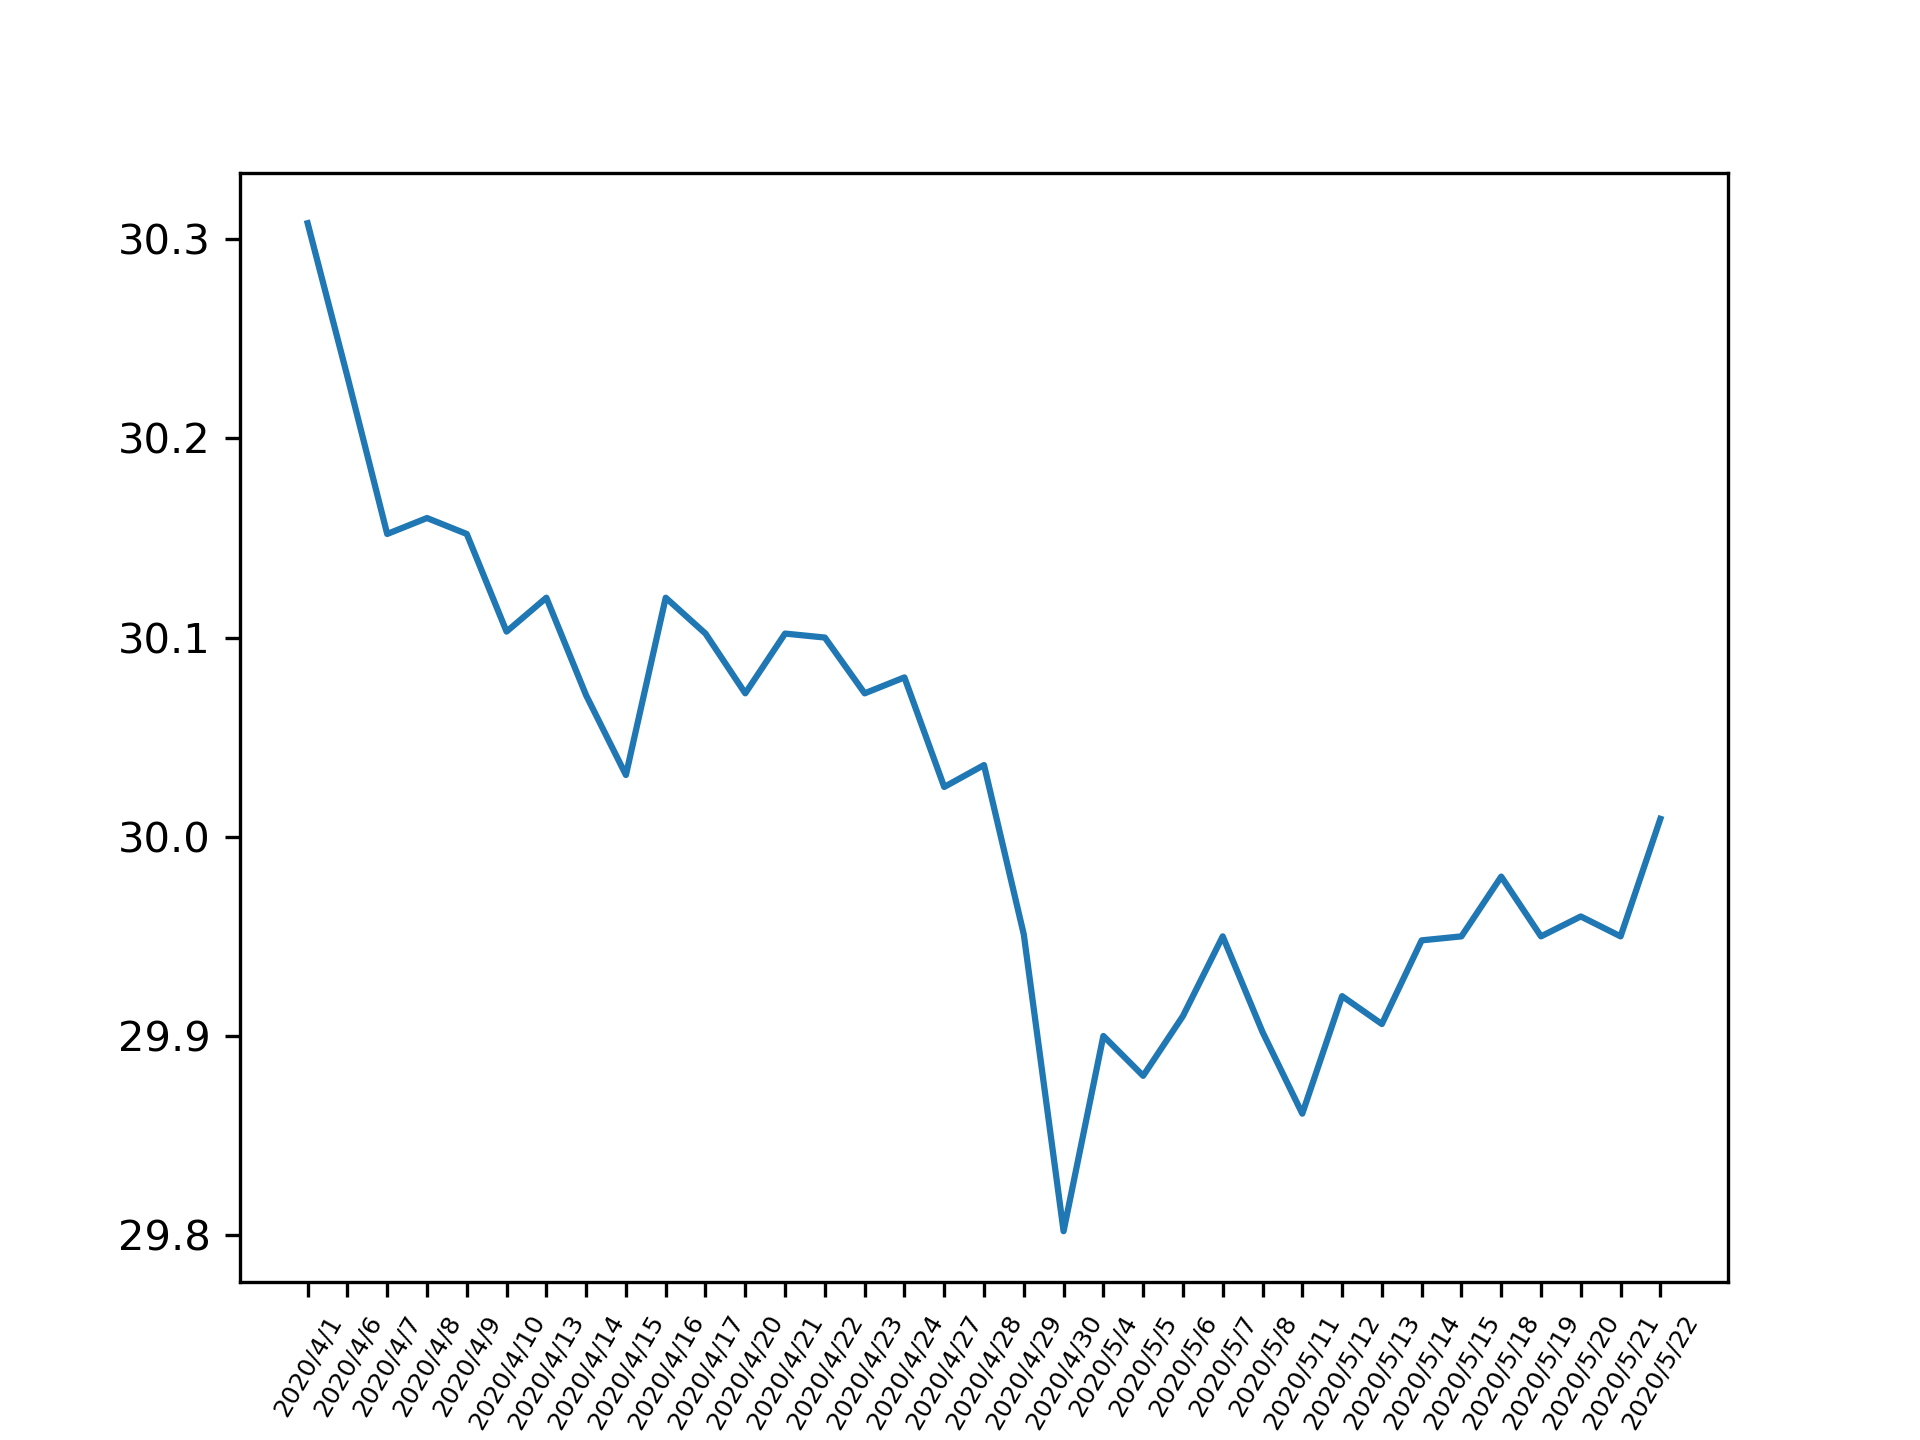
\includegraphics[width=500]{images/jsonLine.png}
\caption{\label{fig:jsonLine}匯率}
\end{figure}
\end{enumerate}
\item 實作 2: \href{https://data.gov.tw/dataset/113063}{澎湖生活博物館每月參觀人次統計資料}
\label{sec:orga58957f}
\lstset{breaklines=true,language=Python,label= ,caption= ,captionpos=b,firstnumber=1,numbers=left}
\begin{lstlisting}
#coding:utf-8
import requests
import pandas as pd
from datetime import datetime

json_url = 'http://opendataap2.penghu.gov.tw/resource/files/2020-01-12/eaa641fc3af66277e60b13201ca11232.json'

response = requests.get(json_url)
jsonRes = response.json()

year = [str(int(i['年度'])+1911) for i in jsonRes]
month = [i['月份'] for i in jsonRes]
visitor = [int(i['人數']) for i in jsonRes]

dates = [x+'/'+y for x, y in zip(year, month)]

from datetime import datetime
#date_object = datetime.strptime(date_str, '%m-%d-%Y').date()

#df['time'] = [pd.to_datetime(i, format='%y%m', errors='ignore') for i in df['date']]
dates = datetime.strptime(dates, '%Y-%m').date()

import matplotlib.pyplot as plt

plt.rcParams['font.family'] = 'cwTeXFangSong'
plt.clf()
plt.bar(dates, visitor)
plt.xticks(rotation=60, fontsize=6)
plt.ylabel('人數')
plt.xlabel('日期')
plt.title('澎湖生活博物館每月參觀人次')
plt.savefig('images/jsonBar.png', dpi=300, bbox_inches='tight')
\end{lstlisting}

\begin{figure}[htbp]
\centering
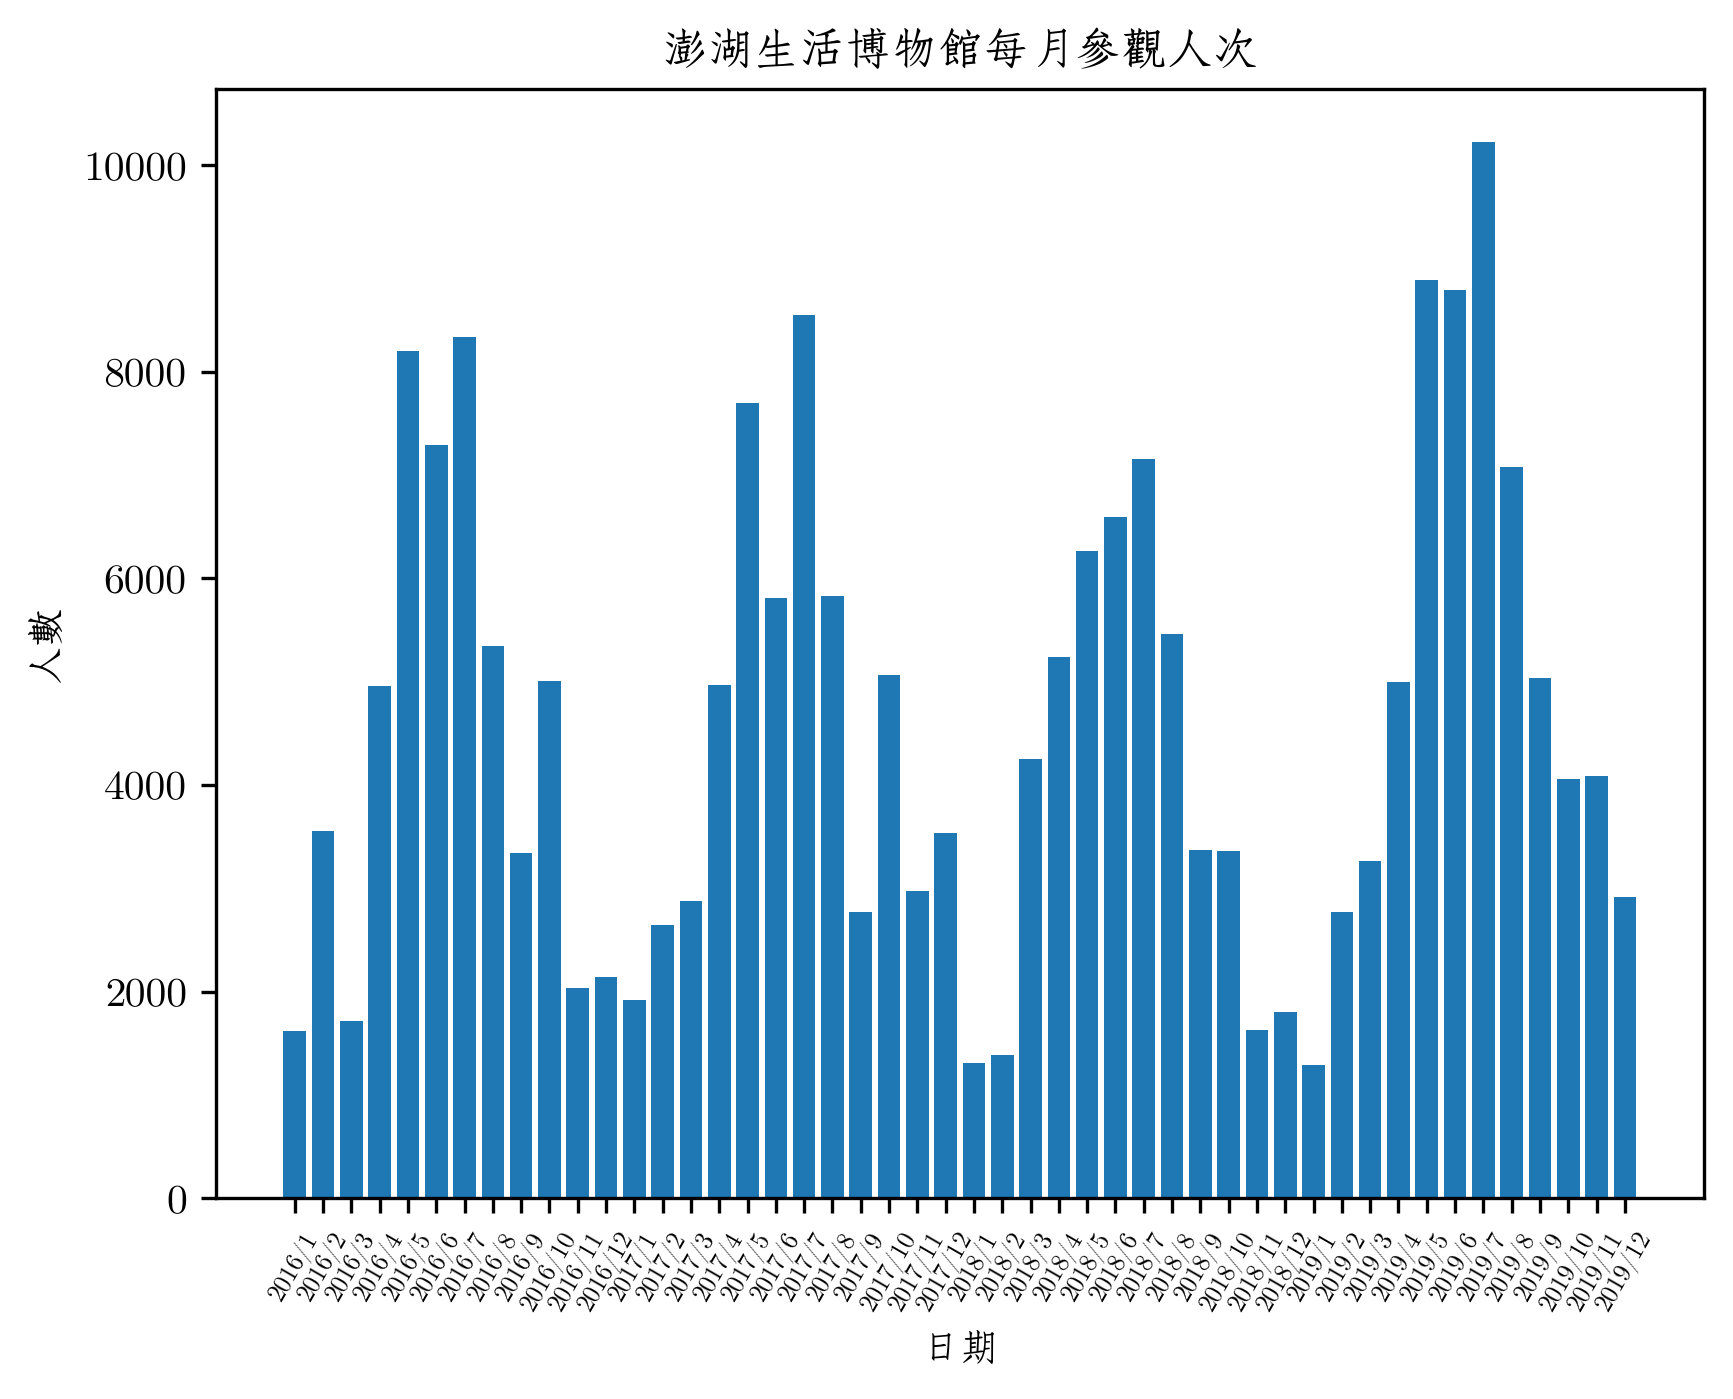
\includegraphics[width=400]{images/jsonBar.png}
\caption{\label{fig:jsonBar}參觀人數}
\end{figure}
\item 實作 3: 學校甄選公告\#1
\label{sec:orgf61d03c}
\lstset{breaklines=true,language=Python,label= ,caption= ,captionpos=b,firstnumber=1,numbers=left}
\begin{lstlisting}
import requests
import json
json_url = 'http://www.kh.edu.tw/json/bulletin/employ/datagrid?page=1&rows=20'
response = requests.get(json_url)

print(response)
# 方法1
jsonRes1 = response.json()
print("========\n", type(jsonRes1))
# 
jsonRes2 = json.loads(response.text)
print("========\n", type(jsonRes2))

print("========\n", jsonRes2)
\end{lstlisting}

\begin{verbatim}
<Response [200]>
========
 <class 'dict'>
========
 <class 'dict'>
========
 {'total': 20, 'rows': [{'author': '大社國中', 'attributes': {'subjects': '家政、歷史、數學、視覺藝術', 'url': 'https://employ.kh.edu.tw/Html/2020/6/大社區109學年度大社國中第1號第1次公告第1次修正簡章.html', 'target': '_blank'}, 'title': '109學年度大社國中第1號第1次公告第1次修正', 'pubDate': '109-06-05'}, {'author': '光華國小', 'attributes': {'subjects': '專任輔導教師', 'url': 'https://employ.kh.edu.tw/Html/2020/6/前鎮區109學年度光華國小第1號第1次公告簡章.html', 'target': '_blank'}, 'title': '109學年度光華國小第1號第1次公告', 'pubDate': '109-06-04'}, {'author': '明誠高中', 'attributes': {'subjects': '國小一般代理教師、國小美術代理教師、國小體育代理教師', 'url': 'https://employ.kh.edu.tw/Html/2020/6/鼓山區109學年度明誠高中第1號第1次公告簡章.html', 'target': '_blank'}, 'title': '109學年度明誠高中第1號第1次公告', 'pubDate': '109-06-01'}, {'author': '八卦國小', 'attributes': {'subjects': '', 'url': 'https://employ.kh.edu.tw/Html/2020/6/仁武區109學年度八卦國小第1號第1次公告簡章.html', 'target': '_blank'}, 'title': '109學年度八卦國小第1號第1次公告', 'pubDate': '109-06-01'}, {'author': '新莊國小', 'attributes': {'subjects': '普通科', 'url': 'https://employ.kh.edu.tw/Html/2020/6/左營區109學年度新莊國小第1號第1次公告簡章.html', 'target': '_blank'}, 'title': '109學年度新莊國小第1號第1次公告', 'pubDate': '109-06-01'}, {'author': '燕巢國中', 'attributes': {'subjects': '資訊科技科(電腦科)', 'url': 'https://employ.kh.edu.tw/Html/2020/6/燕巢區108學年度燕巢國中第14號第12次公告簡章.html', 'target': '_blank'}, 'title': '108學年度燕巢國中第14號第12次公告', 'pubDate': '109-06-05'}, {'author': '前鎮國中', 'attributes': {'subjects': '體育', 'url': 'https://employ.kh.edu.tw/Html/2020/6/前鎮區108學年度前鎮國中第10號第2次公告簡章.html', 'target': '_blank'}, 'title': '108學年度前鎮國中第10號第2次公告', 'pubDate': '109-06-05'}, {'author': '楠梓國中', 'attributes': {'subjects': '音樂專長-豎笛', 'url': 'https://employ.kh.edu.tw/Html/2020/6/楠梓區108學年度楠梓國中第9號第3次公告簡章.html', 'target': '_blank'}, 'title': '108學年度楠梓國中第9號第3次公告', 'pubDate': '109-06-02'}, {'author': '仁武特殊教育學校', 'attributes': {'subjects': '學前教育階段不分類巡迴輔導班', 'url': 'https://employ.kh.edu.tw/Html/2020/5/仁武區108學年度仁武特殊教育學校第7號第5次公告簡章.html', 'target': '_blank'}, 'title': '108學年度仁武特殊教育學校第7號第5次公告', 'pubDate': '109-05-12'}, {'author': '大社國小', 'attributes': {'subjects': '', 'url': 'https://employ.kh.edu.tw/Html/2020/5/大社區108學年度大社國小第7號第3次公告簡章.html', 'target': '_blank'}, 'title': '108學年度大社國小第7號第3次公告', 'pubDate': '109-05-11'}, {'author': '明誠高中', 'attributes': {'subjects': '', 'url': 'https://employ.kh.edu.tw/Html/2020/5/鼓山區108學年度明誠高中第3號第3次公告第1次修正簡章.html', 'target': '_blank'}, 'title': '108學年度明誠高中第3號第3次公告第1次修正', 'pubDate': '109-05-04'}, {'author': '鼓山高中', 'attributes': {'subjects': '', 'url': 'https://employ.kh.edu.tw/Html/2020/5/鼓山區108學年度鼓山高中第11號第3次公告簡章.html', 'target': '_blank'}, 'title': '108學年度鼓山高中第11號第3次公告', 'pubDate': '109-05-04'}, {'author': '南成國小', 'attributes': {'subjects': '兼任特教代課教師', 'url': 'https://employ.kh.edu.tw/Html/2020/5/鳳山區108學年度南成國小第3號第3次公告簡章.html', 'target': '_blank'}, 'title': '108學年度南成國小第3號第3次公告', 'pubDate': '109-05-01'}, {'author': '青山國小', 'attributes': {'subjects': '', 'url': 'https://employ.kh.edu.tw/Html/2020/4/小港區108學年度青山國小第8號第1次公告簡章.html', 'target': '_blank'}, 'title': '108學年度青山國小第8號第1次公告', 'pubDate': '109-04-30'}, {'author': '明宗國小', 'attributes': {'subjects': '', 'url': 'https://employ.kh.edu.tw/Html/2020/4/湖內區108學年度明宗國小第5號第1次公告簡章.html', 'target': '_blank'}, 'title': '108學年度明宗國小第5號第1次公告', 'pubDate': '109-04-30'}, {'author': '大社國中', 'attributes': {'subjects': '國文', 'url': 'https://employ.kh.edu.tw/Html/2020/4/大社區108學年度大社國中第5號第3次公告簡章.html', 'target': '_blank'}, 'title': '108學年度大社國中第5號第3次公告', 'pubDate': '109-04-29'}, {'author': '小港國小', 'attributes': {'subjects': '健康與體適能科', 'url': 'https://employ.kh.edu.tw/Html/2020/4/小港區108學年度小港國小第15號第3次公告簡章.html', 'target': '_blank'}, 'title': '108學年度小港國小第15號第3次公告', 'pubDate': '109-04-21'}, {'author': '小港國小', 'attributes': {'subjects': '一般智能資賦優異資源班', 'url': 'https://employ.kh.edu.tw/Html/2020/4/小港區108學年度小港國小第13號第2次公告簡章.html', 'target': '_blank'}, 'title': '108學年度小港國小第13號第2次公告', 'pubDate': '109-04-18'}, {'author': '鼓山國小', 'attributes': {'subjects': '普通科', 'url': 'https://employ.kh.edu.tw/Html/2020/4/旗山區108學年度鼓山國小第6號第3次公告簡章.html', 'target': '_blank'}, 'title': '108學年度鼓山國小第6號第3次公告', 'pubDate': '109-04-16'}, {'author': '新民國小', 'attributes': {'subjects': '普通科代理(須代導師)', 'url': 'https://employ.kh.edu.tw/Html/2020/4/左營區108學年度新民國小第9號第3次公告簡章.html', 'target': '_blank'}, 'title': '108學年度新民國小第9號第3次公告', 'pubDate': '109-04-14'}]}
\end{verbatim}

\item 實作 4: 學校甄選公告
\label{sec:org3a76ba0}
\lstset{breaklines=true,language=Python,label= ,caption= ,captionpos=b,firstnumber=1,numbers=left}
\begin{lstlisting}
import requests
import json

response = requests.get('http://www.kh.edu.tw/json/bulletin/employ/datagrid?page=1&rows=20')
jsonRes = response.json()
#print(jsonRes['rows'])
for item in jsonRes['rows']:
    print(item['author'], ":", item['title'],"/", item['pubDate'])
#    sortJR = jsonRes['rows']
#    print(type(sortJR))
#
#sortJR.sort(key=lambda x: x['author'], reverse=False)
#for item in sortJR:
#    print(item['author'], ":", item['title'],"/", item['pubDate'])
\end{lstlisting}
\end{enumerate}


\subsection{網路爬蟲}
\label{sec:org937e657}
\begin{enumerate}
\item HTML
\label{sec:org5e0c6a0}
\begin{enumerate}
\item What is HTML
\label{sec:org2bbd55a}
\begin{itemize}
\item \href{https://data.gov.tw/datasets/search?qs=tid\%3A6410}{政府資料開放平台}\\
\item 超文本標記語言（HyperText Markup Language）是一種用於建立網頁的標準標記語言。HTML 是一種基礎技術，常與 CSS、JavaScript 一起被眾多網站用於設計網頁、網頁應用程式以及行動應用程式的使用者介面。\footnote{\href{https://zh.wikipedia.org/zh-tw/HTML}{HTML}\\\label{org0cb91a7}}\\
\item HTML 元素是構建網站的基石。HTML 允許嵌入圖像與物件，並且可以用於建立互動式表單，它被用來結構化資訊——例如標題、段落和列表等等，也可用來在一定程度上描述文件的外觀和語意。\textsuperscript{\ref{org0cb91a7}}\\
\item HTML 的語言形式為<>包圍的 HTML 元素（如<html>），瀏覽器使用 HTML 標籤和指\\
令碼來詮釋網頁內容，但不會將它們顯示在頁面上。 \textsuperscript{\ref{org0cb91a7}}\\
\item 網頁就是由各式標籤 (tag) 所組成的階層式文件。\\
\end{itemize}
\item HTML 範例
\label{sec:org369863a}
\begin{itemize}
\item HTML code\\
\item RESULTS\\
\end{itemize}
\begin{itemize}
\item HTML tree\\
\end{itemize}
\begin{figure}[htbp]
\centering
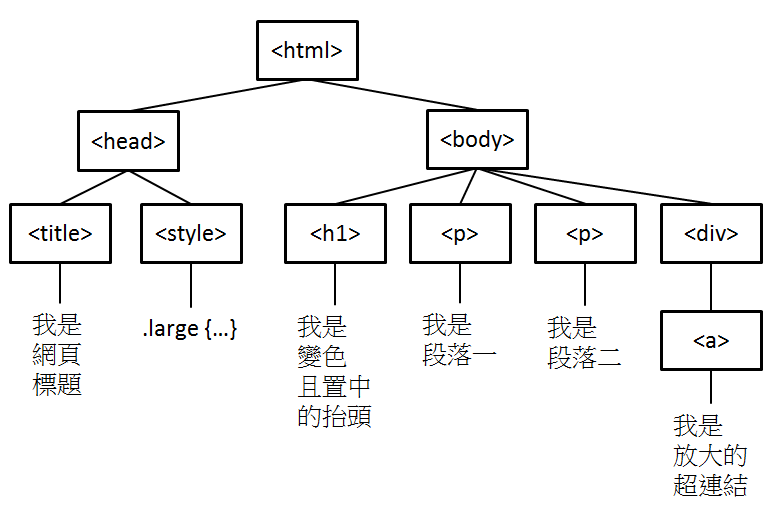
\includegraphics[width=400]{images/html-tree.png}
\caption{\label{fig:HTML-tree}HTML tree}
\end{figure}
\begin{itemize}
\item HTML 文件內不同的標籤 (例如 <title>, <h1>, <p>, <a>\\
\item 不同的標籤有著不同的語義，表示建構網頁用的不同元件，且標籤可以有各種屬性 (例如 id, class, style 等通用屬性, 或 href 等專屬屬性)，\\
\item 因此我們可以用標籤 + 屬性去定位資料所在的區塊並取得資料。\footnote{\href{http://blog.castman.net/\%E6\%95\%99\%E5\%AD\%B8/2016/12/22/python-data-science-tutorial-3.html}{給初學者的 Python 網頁爬蟲與資料分析 (3) 解構並擷取網頁資料}\\}\\
\end{itemize}
\item 爬蟲精神：將程式模仿成一般 user
\label{sec:org3842060}
\begin{enumerate}
\item 原則
\label{sec:orgad16959}
\begin{enumerate}
\item 要抓網路資料，就要先仔細觀察網頁內容\\
\item 要儘量欺騙網站自己是 browser\\
\end{enumerate}
\item 實作範例: 取得 HTML 資料
\label{sec:org527532a}
\begin{enumerate}
\item 第一版
\label{sec:org7727f04}
\lstset{breaklines=true,language=Python,label= ,caption= ,captionpos=b,firstnumber=1,numbers=left}
\begin{lstlisting}
  # 抓取PTT電影版header
  import urllib.request as req
  url = "https://www.ptt.cc/bbs/Stock/index.html"

  with req.urlopen(url) as response:
      data = response.read().decode("utf-8")
  print(data)
\end{lstlisting}
\begin{itemize}
\item 被拒絕原因：這隻程式的行為不像一般使用者，被網站伺服器拒絕。403 Forbidden 是 HTTP 協議中的一個 \href{https://zh.wikipedia.org/zh-tw/HTTP\%E7\%8A\%B6\%E6\%80\%81\%E7\%A0\%81}{HTTP 狀態碼（Status Code）}。可以簡單的理解為沒有權限訪問此站，服務器收到請求但拒絕提供服務\footnote{\href{https://medium.com/ai\%E5\%8F\%8D\%E6\%96\%97\%E5\%9F\%8E/anaconda-miniconda-conda-pip\%E7\%9A\%84\%E7\%9B\%B8\%E4\%BA\%92\%E9\%97\%9C\%E4\%BF\%82-\%E8\%BD\%89\%E8\%BC\%89-a0536f3a257}{Anaconda、Miniconda、Conda、pip的相互關係 (轉載)}\\}。\\
\item urllib.request 是一個用來從 URLs (Uniform Resource Locators)取得資料的 Python 模\\
組。它提供一個了非常簡單的介面能接受多種不同的協議(protocol, 如 http, ftp)， urlopen 函數。\\
\end{itemize}
\item 第二版:加入 headers
\label{sec:org33dada0}
\lstset{breaklines=true,language=Python,label= ,caption= ,captionpos=b,numbers=none}
\begin{lstlisting}
import urllib.request as req
url = "https://www.ptt.cc/bbs/Stock/index.html"
# 幫request加上一個header
request = req.Request(url, headers = {
    "User-Agent":"Mozilla/5.0 (Macintosh; Intel Mac OS X 10.14; rv:72.0) Gecko/20100101 Firefox/72.0"
})

with req.urlopen(request) as response:
    data = response.read().decode("utf-8")
print('所取得的資料型態：',type(data))
print(data[700:1200])
\end{lstlisting}
\begin{results}
所取得的資料型態： <class 'str'>\\
api.js'></script></head>\\
    <body>\\

<div id=``topbar-container''>\\
	<div id=``topbar'' class=``bbs-content''>\\
		<a id=``logo'' href=``\emph{bbs}''>批踢踢實業坊</a>\\
		<span>\&rsaquo;</span>\\
		<a class=``board'' href=``/bbs/Stock/index.html''><span class=``board-label''>看板 </span>Stock</a>\\
		<a class=``right small'' href=``/about.html''>關於我們</a>\\
		<a class=``right small'' href=``/contact.html''>聯絡資訊</a>\\
	</div>\\
</div>\\

<div id=``main-container''>\\
	<div id=``action-bar-container''>\\
		<div class=``action-bar''>\\
			<div class=``btn-group bt\\
\end{results}
\end{enumerate}
\end{enumerate}
\end{enumerate}


\item BeautifulSoup
\label{sec:org544d197}
\begin{enumerate}
\item BeautifulSoup4 簡介
\label{sec:orgc9ab92d}
\begin{itemize}
\item BeautifulSoup4 和 lxml 一樣，Beautiful Soup 也是一個 HTML/XML 的解析器，\\
\item 主要的功能也是如何解析和提取 HTML/XML 資料。\\
\end{itemize}
\item 實作：解析 HTML 資料內容
\label{sec:org7e33db7}
\begin{enumerate}
\item 安裝解析 HTML 所需套件(安裝套件名稱後面有 4)
\label{sec:orga7ac7a0}
\lstset{breaklines=true,language=shell,label= ,caption= ,captionpos=b,numbers=none}
\begin{lstlisting}
pip install beautifulsoup4
\end{lstlisting}
\item 第三版: 解析 HTML
\label{sec:org37c9a21}
\lstset{breaklines=true,language=Python,label= ,caption= ,captionpos=b,firstnumber=1,numbers=left}
\begin{lstlisting}
import urllib.request as req
url = "https://www.ptt.cc/bbs/Stock/index.html"
# 幫request加上一個header
request = req.Request(url, headers = {
    "User-Agent":"Mozilla/5.0 (Macintosh; Intel Mac OS X 10.14; rv:72.0) Gecko/20100101 Firefox/72.0"
})

with req.urlopen(request) as response:
    data = response.read().decode("utf-8")

import bs4
root = bs4.BeautifulSoup(data,"html.parser")
#print(root)
print(type(root))
#print(root.prettify())
print(type(root.prettify()))
##print(root.prettify()[:300])
\end{lstlisting}
\end{enumerate}
\item Beautifulsoup 解析器
\label{sec:orgdbcb8a7}
\begin{itemize}
\item 在上面的語句中，大家可以看到我們使用了一個 html.parser。 這是一個解析器，在構造\\
BeautifulSoup 物件的時候，需要用到解析器。BeautifulSoup 支援 python 內建的解析器\\
和少數第三方解析器。\footnote{\href{https://iter01.com/60617.html}{Python 爬蟲十六式 - 第五式：BeautifulSoup，美味的湯}\\}\\
\item 詳細對比如下：\footnote{\href{https://hiskio.com/courses/112/lectures/3161}{解析器之間的差異}\\}\\
\end{itemize}
\begin{figure}[htbp]
\centering
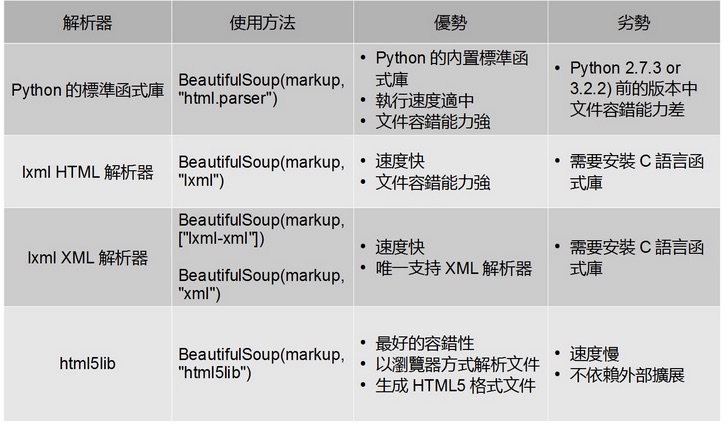
\includegraphics[width=500]{images/parsers.jpg}
\caption{\label{fig:Parsers 比較}Parsers 比較}
\end{figure}
\begin{itemize}
\item 一般來說，對於速度或效能要求不太高的話，還是建議大家使用 html5lib 來進行解析的，\\
但是當規模達到一定程度的時候，解析速度就會影響到整體專案的快慢了，所以如果你對\\
效能有要求的話，還是推薦使用 lxml 來進行解析的。具體的視情況而定吧。\\
\end{itemize}
\item BeautifulSoup4 四大物件
\label{sec:orgf330603}
BeautifulSoup4 將複雜 HTML 文件轉換成一個複雜的樹形結構,每個節點都是 Python 物件,所有物件可以歸納為 4 種:\\
\begin{itemize}
\item Tag: HTML 中的一個個標籤，例如：<title>, <head>, <div>, <link>, <a>\ldots{}，Tag 下\\
擁有許多屬性和方法，和前端類似，例如 a 標籤一定會有它的 href 屬性，某些屬性是某\\
些標籤所獨有的。\\
\item NavigableString: 標籤內部的文字:  .string\\
\item BeautifulSoup: BeautifulSoup 物件就是通過解析網頁所得到的物件，我們的 soup 即\\
是 BeautifulSoup 物件. 可以把它當作 Tag 物件，是一個特殊的 Tag，我們可以分別獲取它的型別，名稱，以及屬性\\
\item Comment: 物件是網頁中的註釋及特殊字串，當你提取網頁中的註釋的時候，它會自動幫你生成 Comment 物件\\
\end{itemize}
\item Tag 物件:
\label{sec:org3de55b9}
\begin{itemize}
\item Tag 物件可以說 BeautifulSoup 中最為重要的物件，通過 BeautifulSoup 來提取資料基本都圍繞著這個物件來進行操作。\\
\item 一個節點中是可以包含多個子節點和多個字串的。例如 html 節點中包含著 head 和 body 節點。\\
所以 BeautifulSoup 就可以將一個 HTML 的網頁用這樣一層層巢狀的節點來進行表示。\\
\item name: 每一個 tag 標籤都有 name 屬性\\
\item attributes: 在 html 中,某個 Tag 可能有多個屬性, Tag 屬性使用和字典一樣的方法取值:\\
\item get\_text(): 通過 get\_text() 方法我們可以獲取某個 Tag 下所有的文字內容：\\
\item find\_all(): 在前面我們講了通過標籤的屬性來進行標籤的訪問的方法，大多都只適用於\\
簡單的一些場景，所以 BeautifulSoup 還提供了搜尋整個文件樹的方法，即 find\_all()。\\
該方法基本適用於任何節點\\
\end{itemize}
\item 第四版：擷取所需資訊
\label{sec:org7dfaa15}
\lstset{breaklines=true,language=Python,label= ,caption= ,captionpos=b,firstnumber=1,numbers=left}
\begin{lstlisting}
import urllib.request as req
url = "https://www.ptt.cc/bbs/Kaohsiung/index.html"
# 幫request加上一個header
request = req.Request(url, headers = {
    "User-Agent":"Mozilla/5.0 (Macintosh; Intel Mac OS X 10.14; rv:72.0) Gecko/20100101 Firefox/72.0"
})

with req.urlopen(request) as response:
    data = response.read().decode("utf-8")

import bs4
root = bs4.BeautifulSoup(data,"html.parser")

titles = root.find_all("div", class_="title")

for t in titles:
    print(t.a)

\end{lstlisting}
\end{enumerate}
\end{enumerate}


\subsection{實作練習}
\label{sec:org17ff951}
\begin{itemize}
\item 由\href{https://data.kcg.gov.tw/dataset?res\_format=JSON}{高雄市政府資料開放平台}找到[高雄市各級學校甄選公告]，線上讀取其線上 JSON 資料，輸\\
出校名及出缺科別。\\
\item 由\href{https://data.gov.tw/}{政府資料開放平台}找到\href{https://data.gov.tw/dataset/107578}{高雄市電動機車充電站名稱及充電站地址}，線上讀取 JSON 檔，列\\
出所有高雄市機車充電站之[計費方式]以及[充電站所在位址]。\\
\item Google 美食達人「壽司羊」，以爬蟲程\\
式列出其部落格(在痞客邦)最近五篇文章\\
的標題以及文章月份。\\

\begin{itemize}
\item 參考解答\\
\end{itemize}
\end{itemize}
\begin{verbatim}
Jun  【高雄食記】初一車輪燒紅豆餅／只要 25 元就可以吃到一大塊的巧克力戚風蛋糕做成的雙重巧克力車輪餅，會牽絲的起司蛋也很好吃((附菜單
Jun  【高雄美食】長代堂食品行／好吃的長崎蜂蜜蛋糕，底下那一層才是配上無糖紅茶的隱藏版超級美味甜點，千萬不要丟掉了！！！
Jun  【冷凍宅配】蝦大俠室內有機養殖 白蝦 草蝦／不出門簡單煮，在家就可以吃到美味的蝦子，不管是烤蝦，水煮蝦都很方便快速。
Jun  【台北美食】地中海牛排館 歐華酒店／超高 CP 值的用餐優惠方案，濕式熟成 50 天肋眼牛排+1000 元送高級雙人房住宿一晚((附菜單
Jun  【高雄食記】玖雞炸物／堅持使用新鮮雞肉，每天到鳳農市場採購，吃得到雞肉鮮味鹽酥雞小店，墨魚黑輪也很好吃，脫油機不油膩((附菜單
\end{verbatim}


\newpage

\section{Python to web}
\label{sec:org261a6c9}
\subsection{Flask}
\label{sec:org2fa2f00}
\lstset{breaklines=true,language=Python,label= ,caption= ,captionpos=b,firstnumber=1,numbers=left}
\begin{lstlisting}
from flask import Flask
app = Flask(__name__)

@app.route("/")
def hello():
    title = "<title>Advanced Materials of Python</title>"
    h1 = "<h1>Python based web</h1>"
    p1 = "<p>Hello python</p>"
    return title+h1+p1

if __name__ == "__main__":
    app.run()
\end{lstlisting}
\begin{figure}[htbp]
\centering
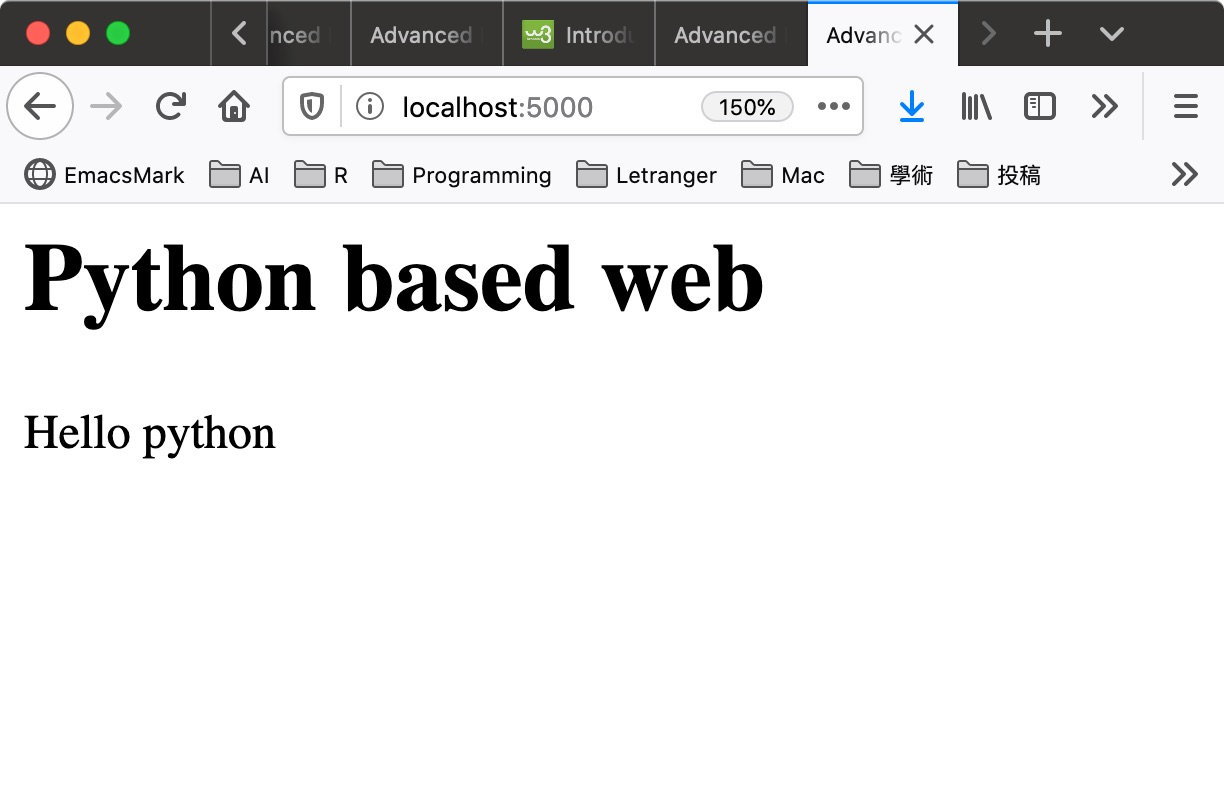
\includegraphics[width=400]{images/FlashSite.jpg}
\caption{\label{fig:PandasPlot-4}Flask Web Site}
\end{figure}

\newpage
\end{document}
